\documentclass[lang=cn,source,XITS,zihao=-4,scheme=chinese,draft]{elegantbook}

\title{空气动力学笔记}
\subtitle{Fundamental of Aerodynamics}

\author{朱荣博}
\bioinfo{简介}{这是一本翻译自Fundamental of Aerodynamics 
的笔记.}

\setcounter{tocdepth}{2}

\logo{logo-blue.png}
\cover{cover.jpg}


%本文档使用的宏包
\usepackage{pdfsync}
\usepackage[overload]{empheq}
\usepackage{tikz}
\usepackage{witharrows}
\usepackage{manfnt}
\usepackage{enumitem}
\usepackage{makeidx}
\usepackage{appendix}
\usepackage{graphicx}
\usepackage{float}
\usepackage{extarrows}
\usepackage{booktabs}%三线表

% 本文档命令
\usepackage{array}
\newcommand{\ccr}[1]{\makecell{{\color{#1}\rule{1cm}{1cm}}}}
%多行公式对齐方框
\newcommand*\widefbox[1]{\fbox{\hspace{1em}#1\hspace{1em}}}
\definecolor{myblue}{rgb}{.8, .8, 1}
\newcommand*\bluebox[1]{%
	\colorbox{myblue}{\hspace{1em}#1\hspace{1em}}
}

%行内数学公式展示模式
\everymath{\displaystyle}
%行间公式允许跨页
\allowdisplaybreaks[4]
%数学算子定义
\DeclareMathOperator*{\dive}{div}
\DeclareMathOperator*{\curl}{curl}
\DeclareMathOperator*{\rot}{rot}
\DeclareMathOperator*{\grad}{grad}
\renewcommand{\grad}{\mathbf{grad}\,}
\renewcommand{\rot}{\mathbf{rot}\,}
\renewcommand{\curl}{\mathbf{curl}\,}

% 修改标题页的橙色带
\definecolor{customcolor}{RGB}{32,178,170}
\colorlet{coverlinecolor}{customcolor}
\usepackage{cprotect}


\begin{document}

\maketitle
\frontmatter

{\centering\color{titleblue}\tableofcontents}

\mainmatter

\part{流体力学基础}
% ! TEX root =../mechanics.tex

\chapter{基础知识}
流体力学认为物体的存在形态只有固态和液态两种
形态,区别在于固体可以通过产生有限的形变来承受
剪切应变.

流体力学作出的基本假设是连续介质假设.即把流体看
成连续不断,没有间隙,始终充满整个空间的连续介质.

控制体是在流场中一个有限封闭区域,这个区域就定义了
一个控制体.控制体可大可小,而这个控制体的封闭表面
就是控制面.换句话说,一个控制体对应着一个控制面.
控制体是固定在流场中的,流体从控制面流入.然后再流
出.当然,控制体也可以随着流体运动,而与周围的流体
没有交换.当控制体的体积趋于微元的控制体的时候,
称为微元体.
\begin{notice}
	微元的体积不能无限小,否则不满足连续介质假设了.
\end{notice}

流体具有压缩性,粘性,传热性等性质.
\begin{enumerate}
	\item 压缩性是指流体可以被压缩,压缩时流体的
	      体积发生变化.此时流体的密度一般也要发生变化.
	\item 粘性是指两层相邻速度不同的流体之间存在
	      着相互牵扯的力,称作粘性力或者内摩擦力.这个
	      力的大小与接触面法线的方向的速度梯度成正比.
	      \[
		      \tau=\mu \frac{\mathrm{d}u}{\mathrm{d}n}
	      \]
	\item 传热性是指流体沿某一方向存在温度梯度时,
	      热量就会从温度高的地方传向温度低的地方.
\end{enumerate}

流体的几个状态参数是压强$P$,温度$T$,密度$\rho$,
速度$\mathbf{V}$,焓值$h$等.这些参数都是关于
$x$,$y$,$z$,$t$的函数,也就是关于坐标和时间的函数.
其中坐标也是时间$t$的函数.

定常是指流体的状态参数和时间变化无关.

\section{流体模型}
\begin{enumerate}
	\item 理想流体 \\
	      不考虑流体的粘性作用的流体模型.
	\item 不可压流体 \\
	      不考虑流体压缩性的流体模型.不可压流体流场中
	      流体的密度是常数,即密度是定常的.
	\item 绝热流体 \\
	      不考虑流体传热性的流体模型,即与外界没有热交换.
\end{enumerate}

\section{量纲分析:白金汉\texorpdfstring{$\mathrm{\Pi}$}{Π}  定理(Dimensional Analysis: The BuckingHam PI Theorem)}
考虑一个给定形状的翼型在一定的攻角下,它受到的总空气动力是$R$。
在物理、直观的基础上,我们期望$R$取决于:
\begin{enumerate}
  \item 自由来流的速度$V_\infty$。
  \item 自由来流的密度$\rho_\infty$。
  \item 流体的黏度。我们已经知道剪切力$\tau$贡献了
    空气动力和空气动力矩,并且$\tau$正比于流体的流动
    的速度梯度。例如,如果给定速度梯度$\frac{\partial u}{\partial y}$,
    那么$\tau=\mu \frac{\partial u}{\partial y}$。这个常数的比例值$\mu$
    就是粘性系数。因此,我们用自由来流的粘性系数$\mu_\infty$来表示粘度对气动力和力矩
    的影响。
  \item 翼型的尺寸,以翼型的参考长度为代表。方便的参考长度是弦长$c$。
  \item 流体的可压性。可压性和遍及全流场的密度变化相关。相应的,可压性
    和流动过程中的声速相关。因此,我们用自由来流的声速$a_\infty$来表示
    可压性对气动力和力矩的影响。
\end{enumerate}

鉴于以上,在没有任何关于$R$变化的先验知识下,我们可以用常识写出:
\[
  R=f(\rho_\infty,V_\infty,c,\mu_\infty,a_\infty)
\]
上式就是一般的函数关系,对于计算$R$就不太实用。原则上,
我们可以将给定的翼型放到风洞中,倾斜到给定的攻角,然后
一次一个地
系统性地测量$R$由于$\rho_\infty$,$V_\infty$,$c$,$\mu_\infty$,
和$a_\infty$的变化而引起的变化。通过交叉绘制这样获得的大量数据,
我们就能提取出对于$R=f(\rho_\infty,V_\infty,c,\mu_\infty,a_\infty)$
的精确函数关系。然而,这肯定是一项艰苦的工作,而且就所需的大量风洞
实验的时间而言,这肯定是昂贵的。幸运的是,首先采用量纲分析的方法,
我们可以简化问题,大大减少我们的时间和精力。

这个方法先定义一组关于气动力和力矩的无量纲参数;这组参数将大大减少
出现在$R=f(\rho_\infty,V_\infty,c,\mu_\infty,a_\infty)$中自变量的
数量。

量纲分析基于一个很明显的事实,即对于真实物理世界中的方程,每一项都必须
具有相同的量纲。例如,如果
\[
  \Psi+\eta+\xi=\Phi
\]
是一个物理关系,那么$\Psi$,$\eta$,$\xi$和$\Phi$必须具有相同的
量纲。否则,我们就会把苹果和橘子加起来。上面那个方程可以通过
除以其中任何一个因子而变成无量纲的,比如$\Phi$:
\[
  \frac{\Psi}{\Phi}+\frac{\eta}{\Phi}+\frac{\xi}{\Phi}=1 
\]
这些思想在白金汉$\Pi$定理中有正式的体现。如下所示。
\begin{notice}
  {\bfseries 白金汉$\Pi$定理}

   设$K$表示描述物理变量所需的基本量纲数量。(在力学中,
   所有的物理变量都可以用质量,长度,时间的量纲来表示;
   因此,$K=3 $。)设$P_1$,$P_2$,$\cdots $,$P_N$表示
   在下述物理关系中的$N$个物理变量
   \[
     f_1(P_1,P_2, \ldots ,P_N)=0
   \]
   然后,上面的物理关系就可以重新表示为$(N-K)$个无量纲积($\Pi$积)的
   关系,
   \[
     f_2(\Pi_1,\Pi_2, \ldots ,\Pi_{N-K})=0
   \]
   在这些无量纲积中,每个$\Pi$积是一个有一组$K$个物理变量
   乘上一个其他物理变量的无量纲积。设$P_1$,$P_2$,$\cdots$,
   $P_K$是被选择的$K$个物理变量,那么:
   \begin{align*}
     \Pi_1&=f_3(P_1,P_2, \ldots ,P_K,P_{K+1})\\ 
     \Pi_2&=f_4(P_1,P_2, \ldots ,P_K,P_{K+2})\\ 
     \Pi_3&=f_5(P_1,P_2, \ldots ,P_K,P_{K+3})\\ 
     \cdots &\cdots \cdots \cdots \cdots \\ 
     \Pi_{N-K}&=f_5(P_1,P_2, \ldots ,P_K,P_N)
   \end{align*}
   重复变量的选择,$P_1$,$P_2$,$\cdots $,$P_K$应该包含用于这个问题
   的所有量纲。当然,这些相互独立的变量应当只在$\Pi$积中出现一次。
\end{notice}

回到,我们考虑的对于给定攻角和给定翼型的气动力和力矩的问题中,
方程
\[
  R=f(\rho_\infty,V_\infty,c,\mu_\infty,a_\infty)
\]
可以写成
\[
  g(R,\rho_\infty,V_\infty,c,\mu_\infty,a_\infty)=0
\]
的形式。根据白金汉$\Pi$定理,基本的量纲是
\begin{align*}
  m&=质量的量纲\\ 
  l&=长度的量纲\\ 
  t&=时间的量纲
\end{align*}
因此,$K=3 $。物理变量和他们的量纲是
\begin{align*}
  [R]&=mlt^{-2}\\ 
  [\rho_\infty]&=ml^{-3}\\ 
  [V_\infty]&=lt^{-1}\\ 
  [c]&=l\\ 
  [\mu_\infty]&=ml^{-1}t^{-1}\\ 
  [a_\infty]&=lt^{-1}
\end{align*}
因此,$N=6$。在上述,气动力$R$的量纲是通过牛顿第二定律获得的,
力=质量$\times$加速度;因此$[R]=mlt^{-2}$。$\mu_\infty$的量纲
是通过它的定义获得的,并且使用了牛顿第二定理。将$\rho_\infty$,
$V_\infty$和$c$作为任意选取$K$个物理变量中的几个。那么
\[
  g(R,\rho_\infty,V_\infty,c,\mu_\infty,a_\infty)=0
\]
可以用$N-K=6-3=3$个无量纲$\Pi$积来重新表示:
\[
  f_2(\Pi_1,P_2,P_3)=0
\]
这些$\Pi$积是:
\begin{align*}
  \Pi_1&=f_3(\rho_\infty,V_\infty,c,R)\\ 
  \Pi_2&=f_4(\rho_\infty,V_\infty,c,\mu_\infty)\\ 
  \Pi_3&=f_5(\rho_\infty,V_\infty,c,a_\infty)
\end{align*}
首先,集中注意在$\Pi_1$上,从上述方程组中的第一个,假定
\[
  \Pi_1=\rho_\infty ^d V_\infty ^b c^e R 
\]
$d$,$b$,$e$是需要找到的指数。在量纲上,上式就是
\[
  [\Pi_1]=(ml^{-3})^d(lt^{-1})^b(l)^e(mlt^{-2})
\]
因为$\Pi_1$是无量纲的,因此,上面方程的右边就必须是无量纲的。
这意味着量纲$m$的指数加起来必须是0,对于量纲$l$和$t$也是
一样的。因此
\begin{align*}
  对于m:& d+l&=0\\ 
  对于l:&-3d+b+e+1&=0\\ 
  对于t:&-b-2&=0
\end{align*}
解上述方程,我们可以得到$d=-1$,$b=-2$和$e=-2$。代入到方程
\[
  \Pi_1=\rho_\infty ^d V_\infty ^b c^e R 
\]
中,得到
\[
  \begin{split} 
    \Pi_1&=R \rho_\infty ^{-1} V_\infty ^{-2} c^{-2}\\ 
         &=\frac{R}{\rho_\infty V_\infty ^2 c^2}
  \end{split}
\]
物理量$\frac{R}{\rho_\infty V_\infty ^2 c^2}$是一个
无量纲的参数,其中$c^2$是一个面积,我们可以将$c^2$替换
为任何我们希望的参考面积(例如机翼的平面面积$S$),并且
$\Pi_1$将依然是无量纲的。更重要的是,我们可以将$\Pi_1$乘
一个纯粹的数量,并且它依然是无量纲的。因此,从上面的方程,
$\Pi_1$可以被定义为
\[
  \Pi_1=\frac{R}{\frac{1}{2}\rho_\infty V_\infty ^2 S}=\frac{R}{q_\infty S}
\]
因此,$\Pi_1$是气动力系数$C_R$。在上式中,$S$就是和给定翼型
有着密切关系的参考面积。

剩余的$\Pi$积可以按照相同的方法求出来。假设
\[
  \Pi_2=\rho_\infty V_\infty ^h c^i \mu_\infty ^j
\]
参考上述的分析,我们可以获得
\[
  [\Pi_2]=(ml^{-3})(lt^{-1})^h(l)^i(ml^{-1}t^{-1})^j
\]
因此,
\begin{align*}
  1+j&=0\\ 
  -3+h+i-j&=0\\ 
  -h-j&=0
\end{align*}
因此,$j=-1$,$h=1$,和$i=1$。代入到上式中就有
\[
  \Pi_2=\frac{\rho_\infty V_\infty c}{\mu_\infty}
\]
这个无量纲结合体被定义为雷诺数。雷诺数是在流动中物理测量的惯性力和
粘性力的比值,并且在流体力学中是最有力的参数之一。

再假设
\begin{align*}
  \Pi_3=V_\infty \rho_\infty ^k c^r a_\infty ^s \\ 
  [\Pi_3]=(lt^{-1})(ml^{-3})^k(l)^r(lt^{-1})^s 
\end{align*}
同样得到方程组
\[
  \begin{split}
    k&=0\\ 
    1-3k+r+s&=0\\ 
    -1-s&=0
  \end{split}
\]
因此,$k=0$,$s=-1$,$r=0$。代入到上式有,
\[
  \Pi_3=\frac{V_\infty}{a_\infty}
\]
这个无量纲量被定义为马赫数$M=\frac{V_\infty}{a_\infty}$。
马赫数是流动速度和声速的比值;它是研究气体动力的强有力
的参数。

无量纲分析的结果可以被写成如下
\begin{align*}
  f_2(\frac{R}{\frac{1}{2}\rho_\infty v_\infty ^2 S},
  \frac{\rho_\infty V_\infty c }{\mu_\infty },
  \frac{V_\infty }{a_\infty})=0\\ 
  f_2(C_R,Re,M_\infty)=0\\ 
  C_R=f_6(Re,M_\infty)
\end{align*}
这是一个重要的结果!在一开始,$R$被表示成有5个独立变量的
一般函数关系。然而,我们的量纲分析已经表示成:
\begin{enumerate}
  \item $R$可以被表示为无量纲气动力系数的项,
    $C_R=\frac{R}{\frac{1}{2}\rho_\infty V_\infty ^2 S }$。
  \item $C_R$只是Re和$M_\infty$的函数。 
\end{enumerate}
因此,通过用白金汉$\Pi$定理,可以减少不相互独立变量的数目,即
从5个变量减少成2个变量。现在,如果我们希望对一个给定的翼型在一个
固定的攻角下,做一系列风洞测试,我们只需要变化雷诺数和马赫数去获得
数据得到$R$的计算公式。通过很少的分析,我们就已经节约了很多努力和大量
的风洞时间。更重要的是,我们定义了两个控制流动的
无量纲参数,雷诺数和马赫数。它们叫做{\bfseries 相似参数(similarity 
parameters)}。因为升力和阻力都是总空气动力的分量,因此
\[
  C_L=f_7(Re,M_\infty)
\]
\[
  C_D=f_8(Re,M_\infty)
\]
更重要的是,这个关系对于气动力矩也成立,即
\[
  C_M=f_9(Re,M_\infty)
\]
请记住,上述关系是对于给定翼型在固定攻角下成立的。如果$\alpha$
是允许可变的,那么$C_L$,$C_D$,$C_M$都是依赖于变量$\alpha$的。
因此
\[
  C_L=f_{10}(Re,M_\infty,\alpha)
\]
\[
  C_D=f_{11}(Re,M_\infty,\alpha)
\]
\[
  C_M=f_{12}(Re,M_\infty,\alpha)
\]
上述方程的前提是假定翼型形状是给定的。大量的理论和实验
都聚焦在获取对于固定翼型形状的清晰的表达式,即上述方程。

\section{气动力和气动力矩}
\label{气动力和气动力矩}
气动力的来源主要有两部分,即:
\begin{enumerate}
	\item 作用在机翼表面的压强力。
	\item 作用在机翼表面的剪切力。
\end{enumerate}
无论机翼形状多么复杂,气动力和气动力矩总是
来源于上述两个方面。一般把垂直于机翼表面的
力称作{\bfseries 压强力(pressure stress)}。平行于机翼表面的
力称作{\bfseries 剪切力(shear stress)}。将压强力和剪切力
沿机翼表面积分,得到总空气动力$R$和总空气
动力矩$M$,并将总空气动力的作用点叫做{\bfseries 压心}。
如下图\ref{fig:airfoil force},将机翼远前方的气流速度记作$V_\infty$,
远离机翼的流体也叫做{\bfseries 自由来流(freestream)},因此,
$V_\infty$也叫做自由来流速度。

\begin{figure}[!ht]
	\centering
	% ! TEX root = ./introductory_thoughts.tex
\tikzset{every picture/.style={line width=0.75pt}} %set default line width to 0.75pt        

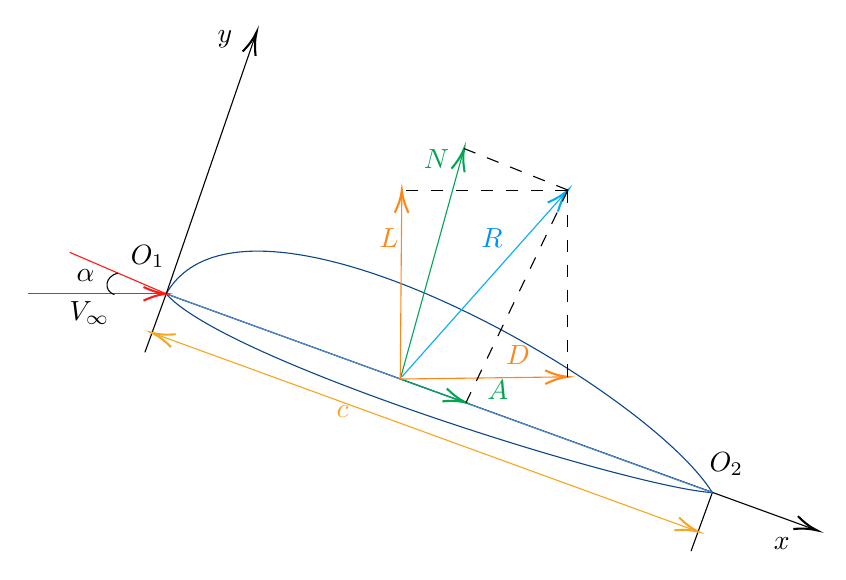
\begin{tikzpicture}[x=0.75pt,y=0.75pt,yscale=-1,xscale=1]
	%uncomment if require: \path (0,353); %set diagram left start at 0, and has height of 353

	%Straight Lines [id:da1842109967268275] 
	\draw    (186.47,136.04) -- (498.12,249.32) ;
	\draw [shift={(500,250)}, rotate = 199.97] [color={rgb, 255:red, 0; green, 0; blue, 0 }  ][line width=0.75]    (10.93,-3.29) .. controls (6.95,-1.4) and (3.31,-0.3) .. (0,0) .. controls (3.31,0.3) and (6.95,1.4) .. (10.93,3.29)   ;
	%Curve Lines [id:da035648358588663775] 
	\draw [color={rgb, 255:red, 14; green, 70; blue, 139 }  ,draw opacity=1 ]   (186.47,136.04) .. controls (224.32,69.81) and (417.44,180.11) .. (449.59,231.81) ;
	%Curve Lines [id:da2965896641352135] 
	\draw [color={rgb, 255:red, 14; green, 70; blue, 139 }  ,draw opacity=1 ]   (186.47,136.04) .. controls (214.79,168.5) and (409.77,229.25) .. (449.59,231.81) ;
	%Straight Lines [id:da05743983968805111] 
	\draw [color={rgb, 255:red, 74; green, 144; blue, 226 }  ,draw opacity=1 ]   (186.47,136.04) -- (449.59,231.81) ;
	%Straight Lines [id:da10439448052891231] 
	\draw    (449.59,231.81) -- (439.33,260) ;
	%Straight Lines [id:da788041337249308] 
	\draw    (186.47,136.04) -- (176.21,164.23) ;
	%Straight Lines [id:da7611175858700716] 
	\draw [color={rgb, 255:red, 245; green, 166; blue, 35 }  ,draw opacity=1 ]   (292.4,195.88) -- (440.87,249.92) ;
	\draw [shift={(442.75,250.6)}, rotate = 200] [color={rgb, 255:red, 245; green, 166; blue, 35 }  ,draw opacity=1 ][line width=0.75]    (10.93,-3.29) .. controls (6.95,-1.4) and (3.31,-0.3) .. (0,0) .. controls (3.31,0.3) and (6.95,1.4) .. (10.93,3.29)   ;
	%Straight Lines [id:da4556885360753773] 
	\draw [color={rgb, 255:red, 245; green, 166; blue, 35 }  ,draw opacity=1 ][fill={rgb, 255:red, 245; green, 166; blue, 35 }  ,fill opacity=1 ]   (292.4,195.88) -- (181.51,155.52) ;
	\draw [shift={(179.63,154.84)}, rotate = 20] [color={rgb, 255:red, 245; green, 166; blue, 35 }  ,draw opacity=1 ][line width=0.75]    (10.93,-3.29) .. controls (6.95,-1.4) and (3.31,-0.3) .. (0,0) .. controls (3.31,0.3) and (6.95,1.4) .. (10.93,3.29)   ;
	%Straight Lines [id:da3164870624705869] 
	\draw [color={rgb, 255:red, 0; green, 166; blue, 82 }  ,draw opacity=1 ]   (299.24,177.09) -- (329.47,67.96) ;
	\draw [shift={(330,66.04)}, rotate = 105.48] [color={rgb, 255:red, 0; green, 166; blue, 82 }  ,draw opacity=1 ][line width=0.75]    (10.93,-3.29) .. controls (6.95,-1.4) and (3.31,-0.3) .. (0,0) .. controls (3.31,0.3) and (6.95,1.4) .. (10.93,3.29)   ;
	%Straight Lines [id:da47805468728724976] 
	\draw [color={rgb, 255:red, 0; green, 166; blue, 82 }  ,draw opacity=1 ]   (299.24,177.09) -- (329.03,187.78) ;
	\draw [shift={(330.91,188.45)}, rotate = 199.74] [color={rgb, 255:red, 0; green, 166; blue, 82 }  ,draw opacity=1 ][line width=0.75]    (10.93,-3.29) .. controls (6.95,-1.4) and (3.31,-0.3) .. (0,0) .. controls (3.31,0.3) and (6.95,1.4) .. (10.93,3.29)   ;
	%Straight Lines [id:da9044725657133146] 
	\draw [color={rgb, 255:red, 255; green, 25; blue, 25 }  ,draw opacity=1 ]   (120,136.04) -- (184.47,136.04) ;
	\draw [shift={(186.47,136.04)}, rotate = 180.01] [color={rgb, 255:red, 255; green, 25; blue, 25 }  ,draw opacity=1 ][line width=0.75]    (10.93,-3.29) .. controls (6.95,-1.4) and (3.31,-0.3) .. (0,0) .. controls (3.31,0.3) and (6.95,1.4) .. (10.93,3.29)   ;
	%Straight Lines [id:da007233215583360764] 
	\draw [color={rgb, 255:red, 255; green, 134; blue, 24 }  ,draw opacity=1 ]   (299.24,177.09) -- (299.98,88.04) ;
	\draw [shift={(300,86.04)}, rotate = 90.48] [color={rgb, 255:red, 255; green, 134; blue, 24 }  ,draw opacity=1 ][line width=0.75]    (10.93,-3.29) .. controls (6.95,-1.4) and (3.31,-0.3) .. (0,0) .. controls (3.31,0.3) and (6.95,1.4) .. (10.93,3.29)   ;
	%Straight Lines [id:da3618051683565324] 
	\draw [color={rgb, 255:red, 255; green, 134; blue, 24 }  ,draw opacity=1 ]   (299.24,177.09) -- (378,176.06) ;
	\draw [shift={(380,176.04)}, rotate = 179.26] [color={rgb, 255:red, 255; green, 134; blue, 24 }  ,draw opacity=1 ][line width=0.75]    (10.93,-3.29) .. controls (6.95,-1.4) and (3.31,-0.3) .. (0,0) .. controls (3.31,0.3) and (6.95,1.4) .. (10.93,3.29)   ;
	%Straight Lines [id:da04699365108287412] 
	\draw [color={rgb, 255:red, 0; green, 174; blue, 247 }  ,draw opacity=1 ]   (300,176.04) -- (378.67,87.53) ;
	\draw [shift={(380,86.04)}, rotate = 131.63] [color={rgb, 255:red, 0; green, 174; blue, 247 }  ,draw opacity=1 ][line width=0.75]    (10.93,-3.29) .. controls (6.95,-1.4) and (3.31,-0.3) .. (0,0) .. controls (3.31,0.3) and (6.95,1.4) .. (10.93,3.29)   ;
	%Straight Lines [id:da6731669887886254] 
	\draw  [dash pattern={on 4.5pt off 4.5pt}]  (380,86.04) -- (300,86.04) ;
	%Straight Lines [id:da61043324884377] 
	\draw  [dash pattern={on 4.5pt off 4.5pt}]  (380,86.04) -- (380,176.04) ;
	%Straight Lines [id:da16658450416549608] 
	\draw  [dash pattern={on 4.5pt off 4.5pt}]  (380,86.04) -- (330,66.04) ;
	%Straight Lines [id:da03948089339816563] 
	\draw  [dash pattern={on 4.5pt off 4.5pt}]  (380,86.04) -- (330.91,188.45) ;
	%Straight Lines [id:da8326545905273048] 
	\draw [color={rgb, 255:red, 255; green, 25; blue, 25 }  ,draw opacity=1 ]   (140,116.04) -- (186.47,136.04) ;
	%Curve Lines [id:da294193336921325] 
	\draw    (163.24,126.04) .. controls (157.01,127.45) and (156.01,134.45) .. (161.51,136.45) ;
	%Straight Lines [id:da6512080695488691] 
	\draw    (186.47,136.04) -- (229.35,11.89) ;
	\draw [shift={(230,10)}, rotate = 109.05] [color={rgb, 255:red, 0; green, 0; blue, 0 }  ][line width=0.75]    (10.93,-3.29) .. controls (6.95,-1.4) and (3.31,-0.3) .. (0,0) .. controls (3.31,0.3) and (6.95,1.4) .. (10.93,3.29)   ;


	% Text Node
	\draw (210,8.07) node [anchor=north west][inner sep=0.75pt]    {$y$};
	% Text Node
	\draw (478,252.4) node [anchor=north west][inner sep=0.75pt]    {$x$};
	% Text Node
	\draw (267.33,188.73) node [anchor=north west][inner sep=0.75pt]  [color={rgb, 255:red, 245; green, 166; blue, 35 }  ,opacity=1 ]  {$c$};
	% Text Node
	\draw (142,123) node [anchor=north west][inner sep=0.75pt]    {$\alpha $};
	% Text Node
	\draw (168.07,111.32) node [anchor=north west][inner sep=0.75pt]  [rotate=-359.37]  {$O_{1}$};
	% Text Node
	\draw (447,211.4) node [anchor=north west][inner sep=0.75pt]    {$O_{2}$};
	% Text Node
	\draw (337,103.4) node [anchor=north west][inner sep=0.75pt]  [color={rgb, 255:red, 0; green, 147; blue, 247 }  ,opacity=1 ]  {$R$};
	% Text Node
	\draw (288,103.4) node [anchor=north west][inner sep=0.75pt]  [color={rgb, 255:red, 255; green, 134; blue, 24 }  ,opacity=1 ]  {$L$};
	% Text Node
	\draw (349,159.73) node [anchor=north west][inner sep=0.75pt]  [color={rgb, 255:red, 255; green, 134; blue, 24 }  ,opacity=1 ]  {$D$};
	% Text Node
	\draw (340,176.4) node [anchor=north west][inner sep=0.75pt]  [color={rgb, 255:red, 0; green, 166; blue, 82 }  ,opacity=1 ]  {$A$};
	% Text Node
	\draw (309.33,65.07) node [anchor=north west][inner sep=0.75pt]  [color={rgb, 255:red, 0; green, 166; blue, 82 }  ,opacity=1 ]  {$N$};
	% Text Node
	\draw (138.67,138.4) node [anchor=north west][inner sep=0.75pt]    {$V_{\infty }$};

\end{tikzpicture}

  \caption{机翼气动力图}
  \label{fig:airfoil force}
\end{figure}

把总空气动力$R$在垂直于自由来流速度$V_\infty$
方向上的分量叫做{\bfseries 升力(lift)},
记作$L$。把总空气动
力$R$在平行于自由来流速度$V_\infty$方向的分
量叫做{\bfseries 阻力(drag)},记作$D$。

总空气动力$R$的大小和自由来流的密度,速度,机翼
的弦长,自由来流的粘性,自由来流的声速大小有关,即
\[
  R=f(\rho_\infty,V_\infty,c,\mu_\infty,a_\infty)
\]
也可以写成
\[
  C_R=f(\mathrm{Re},M_\infty)
\]
其中
\[
  C_R=\frac{R}{\frac{1}{2}\rho_\infty V_\infty ^2 S}
\]

{\bfseries 弦长(chord)} $c$是从机翼的前缘点到后缘点的直线距离。
有时,$R$可以被分解成垂直弦长的正压力$N$和
平行于弦长的轴向力$A$。

{\bfseries 攻角(angle of attack)} $\alpha$是弦长$c$
和自由来流速度$V_\infty$的夹角,又称为飞行迎角。
同时,攻角也是$L$和$N$的夹角或$D$和$A$的夹角。
它们之间的几何关系是
\begin{align*}
	L & =N \cos \alpha -A \sin \alpha \\
	D & =N \sin \alpha +A \cos \alpha
\end{align*}

自由来流的速度和密度分别是$V_\infty$,$\rho_\infty$。
自由来流的动压$q_\infty$就是
\[
  q_\infty=\frac{1}{2}\rho_\infty V_\infty ^2
\]
另外,给出特征面积$S$和特征长度$l$,具体见下图\ref{fig:reference_aera},
给出气动力
系数和气动力矩系数的计算公式:
\begin{align*}
  C_L&=\frac{L}{q_\infty S}\\ 
  C_D&=\frac{D}{q_\infty S}\\ 
  C_M&=\frac{M}{q_\infty S l}
\end{align*}
由于,升力和阻力都是总空气动力的分量,因此
\begin{align*}
  C_L&=f_1(\mathrm{Re},M_\infty,\alpha)\\ 
  C_D&=f_2(\mathrm{Re},M_\infty,\alpha)\\ 
  C_M&=f_3(\mathrm{Re},M_\infty,\alpha)
\end{align*}
\begin{notice}
下标$\infty$表示单位翼展长度上的气动力和气动力矩,
与三维气动力和气动力矩的符号区分开。
\end{notice}
\begin{figure}[!ht]
  \center
  % ! TEX root = ./introductory_thoughts.tex

\tikzset{every picture/.style={line width=0.75pt}} %set default line width to 0.75pt        

\begin{tikzpicture}[x=0.75pt,y=0.75pt,yscale=-1,xscale=1]
%uncomment if require: \path (0,329); %set diagram left start at 0, and has height of 329

%Straight Lines [id:da8457061326808677] 
\draw    (110,110) -- (280,80) ;
%Straight Lines [id:da3677073589615114] 
\draw    (280,80) -- (450,110) ;
%Straight Lines [id:da6827512794214365] 
\draw    (110,140) -- (280,170) ;
%Straight Lines [id:da9375160540186047] 
\draw    (450,140) -- (280,170) ;
%Curve Lines [id:da7430342160557699] 
\draw    (110,140) .. controls (100.51,130.41) and (101.51,118.91) .. (110,110) ;
%Curve Lines [id:da9117728038874897] 
\draw    (450,110) .. controls (459.51,119.91) and (459.51,130.41) .. (450,140) ;
%Straight Lines [id:da8154691434530481] 
\draw [line width=1.5]    (280,10) -- (280,67) ;
\draw [shift={(280,70)}, rotate = 270] [color={rgb, 255:red, 0; green, 0; blue, 0 }  ][line width=1.5]    (14.21,-4.28) .. controls (9.04,-1.82) and (4.3,-0.39) .. (0,0) .. controls (4.3,0.39) and (9.04,1.82) .. (14.21,4.28)   ;
%Straight Lines [id:da22105158102358313] 
\draw    (340,90) -- (340,160) ;
%Shape: Brace [id:dp9292741196091328] 
\draw   (340.01,90.91) .. controls (335.34,90.91) and (333.01,93.24) .. (333.01,97.91) -- (333.01,114.91) .. controls (333.01,121.58) and (330.68,124.91) .. (326.01,124.91) .. controls (330.68,124.91) and (333.01,128.24) .. (333.01,134.91)(333.01,131.91) -- (333.01,151.91) .. controls (333.01,156.58) and (335.34,158.91) .. (340.01,158.91) ;
%Shape: Circle [id:dp8151008192668772] 
\draw   (249,210.91) .. controls (249,193.79) and (262.88,179.91) .. (280,179.91) .. controls (297.12,179.91) and (311,193.79) .. (311,210.91) .. controls (311,228.03) and (297.12,241.91) .. (280,241.91) .. controls (262.88,241.91) and (249,228.03) .. (249,210.91) -- cycle ;
%Straight Lines [id:da5614464812389859] 
\draw [line width=1.5]    (181.51,210.41) -- (237,210.02) ;
\draw [shift={(240,210)}, rotate = 179.59] [color={rgb, 255:red, 0; green, 0; blue, 0 }  ][line width=1.5]    (14.21,-4.28) .. controls (9.04,-1.82) and (4.3,-0.39) .. (0,0) .. controls (4.3,0.39) and (9.04,1.82) .. (14.21,4.28)   ;
%Straight Lines [id:da04411805177983297] 
\draw    (280,210.91) -- (280,181.91) ;
\draw [shift={(280,179.91)}, rotate = 90] [color={rgb, 255:red, 0; green, 0; blue, 0 }  ][line width=0.75]    (10.93,-3.29) .. controls (6.95,-1.4) and (3.31,-0.3) .. (0,0) .. controls (3.31,0.3) and (6.95,1.4) .. (10.93,3.29)   ;
%Straight Lines [id:da15782518028669035] 
\draw    (280,210) -- (280,239.91) ;
\draw [shift={(280,241.91)}, rotate = 270] [color={rgb, 255:red, 0; green, 0; blue, 0 }  ][line width=0.75]    (10.93,-3.29) .. controls (6.95,-1.4) and (3.31,-0.3) .. (0,0) .. controls (3.31,0.3) and (6.95,1.4) .. (10.93,3.29)   ;

% Text Node
\draw (251,32.4) node [anchor=north west][inner sep=0.75pt]    {$V_{\infty }$};
% Text Node
\draw (316,115.4) node [anchor=north west][inner sep=0.75pt]    {$c$};
% Text Node
\draw (120,119.4) node [anchor=north west][inner sep=0.75pt]    {$\text{面积}S$};
% Text Node
\draw (194,211.4) node [anchor=north west][inner sep=0.75pt]    {$V_{\infty }$};
% Text Node
\draw (268,203.4) node [anchor=north west][inner sep=0.75pt]    {$d$};
% Text Node
\draw (321,213.4) node [anchor=north west][inner sep=0.75pt]    {$S=\text{横截面积}=\frac{\pi d^2}{4}$};
% Text Node
\draw (321,242.4) node [anchor=north west][inner sep=0.75pt]    {$l=d=\text{直径}$};
% Text Node
\draw (400,153.4) node [anchor=north west][inner sep=0.75pt]    {$S=\text{翼展平面面积}$};
% Text Node
\draw (400,182.4) node [anchor=north west][inner sep=0.75pt]    {$l=c=\text{弦长}$};


\end{tikzpicture}

  \caption{机翼特征尺寸}
  \label{fig:reference_aera}
\end{figure}
对于二维平面的机翼,也就是单位长度上的
升力$L$和阻力$D$,力矩$M$。特征面积
$S=c(1)=c$,
上述气动力系数和气动力矩系数
写成
\begin{align*}
  c_l&=\frac{L}{q_\infty c}\\ 
  c_d&=\frac{D}{q_\infty c}\\ 
  c_m&=\frac{M}{q_\infty c^2}
\end{align*}

{\bfseries 压强系数}是自由来流的压强$P_\infty$和
与机翼上压强$P$的差值与动压的比值。即
\[
  C_P=\frac{P-P_\infty}{q_\infty}
\]
表面摩擦系数
\[
  C_f=\frac{\tau}{q_\infty}
\]

{\bfseries 升阻比}是机翼的升力和阻力的比值即
\[
  \frac{L}{D}=\frac{C_L}{C_D}
\]

{\bfseries 压心(center of pressure)}是总空气动力的作用点,同时对压心取矩
为0。
\begin{notice}
对于压心的定义可以参考如下:\\ 
It is the location where the resultant of a distributed load effectively acts on the
body.If moments were taken about the center of pressure, the integrated effect of
the distributed loads would be zero。
\end{notice}

如果将气动力平移到机翼{\bfseries 前缘点(leading edge)}位置
(图\ref{fig:CenterOfPressure}),
同时产生一个力矩$M_{LE}$,称为{\bfseries 前缘力矩},那么压心的位置$x_{cp}$由
下式给出
\[
  x_{cp}=-\frac{M_{LE}}{L}
\]
\begin{figure}[!ht]
  \center
  % ! TEX root = ./introductory_thoughts.tex

\tikzset{every picture/.style={line width=0.75pt}} %set default line width to 0.75pt        

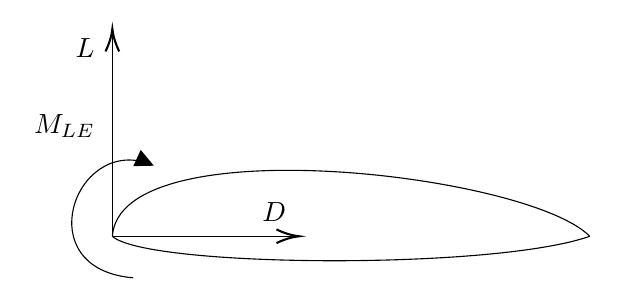
\begin{tikzpicture}[x=0.75pt,y=0.75pt,yscale=-1,xscale=1]
%uncomment if require: \path (0,300); %set diagram left start at 0, and has height of 300

%Curve Lines [id:da6282201102429681] 
\draw    (200,150) .. controls (203.67,97) and (400.18,119.75) .. (430,150) ;
%Curve Lines [id:da8779431608993546] 
\draw    (200,150) .. controls (216.34,165) and (383.51,166.41) .. (430,150) ;
%Straight Lines [id:da2590905789853304] 
\draw    (200,150) -- (200,52) ;
\draw [shift={(200,50)}, rotate = 90] [color={rgb, 255:red, 0; green, 0; blue, 0 }  ][line width=0.75]    (10.93,-3.29) .. controls (6.95,-1.4) and (3.31,-0.3) .. (0,0) .. controls (3.31,0.3) and (6.95,1.4) .. (10.93,3.29)   ;
%Straight Lines [id:da6275146811901227] 
\draw    (200,150) -- (288,150) ;
\draw [shift={(290,150)}, rotate = 180] [color={rgb, 255:red, 0; green, 0; blue, 0 }  ][line width=0.75]    (10.93,-3.29) .. controls (6.95,-1.4) and (3.31,-0.3) .. (0,0) .. controls (3.31,0.3) and (6.95,1.4) .. (10.93,3.29)   ;
%Curve Lines [id:da7637601528691369] 
\draw    (210,170) .. controls (159.47,165.85) and (181.66,102.38) .. (217.24,114.89) ;
\draw [shift={(220,116)}, rotate = 204.48] [fill={rgb, 255:red, 0; green, 0; blue, 0 }  ][line width=0.08]  [draw opacity=0] (8.93,-4.29) -- (0,0) -- (8.93,4.29) -- cycle    ;

% Text Node
\draw (181,53.4) node [anchor=north west][inner sep=0.75pt]    {$L$};
% Text Node
\draw (271,132.4) node [anchor=north west][inner sep=0.75pt]    {$D$};
% Text Node
\draw (161,90) node [anchor=north west][inner sep=0.75pt]    {$M_{LE}$};


\end{tikzpicture}

  \caption{前缘力矩}
  \label{fig:CenterOfPressure}
\end{figure}

一般规定,使得飞机抬头的力矩为正,使得飞机低头的力矩为负。
或者说,使得飞行迎角增大的力矩为正。

当气动力$N$和$A$减小时,$x_{cp}$增大。当气动力趋近于0时,
压心就移动到无穷远处了。



%场论
% ! TEX root = ../mechanics.tex

\chapter{场论基础知识}

在介绍场论基础知识之前,这里不加约定地
将速度场$\mathbf{V}$认为是矢量场,而密度场
$\rho$,压强场$P$,温度场$T$等是标量场.如无
特殊说明,均认为上述参数是定常的.在引入新的
场变量时,用加粗字母表示矢量,不加粗字母表示数量.
比如$\mathbf{V}$时矢量场,但是$V$时标量场.
\section{梯度,旋度,散度}
\subsection{梯度计算}
对于标量场 $\rho=\rho(x,y,z)$,它的
梯度是
$$
    \nabla \rho=\frac{\partial \rho}{\partial x}\mathbf{i}
    +\frac{\partial \rho}{\partial y}\mathbf{j}
    +\frac{\partial \rho}{\partial z}\mathbf{k}
$$
标量场的梯度是一个向量,是这个标量函数下降最快的方向.
记作$\grad \rho$.

\subsection{旋度计算}
对于矢量场 $\mathbf{V}=u \mathbf{i}+
v \mathbf{j} +w \mathbf{k}$,它的旋度是
\begin{equation*}
    \nabla\times \mathbf{V}=
    \begin{vmatrix}
        \mathbf{i} & \mathbf{j}                   & \mathbf{k} \\
        \frac{\partial}{\partial x}
                   & \frac{\partial }{\partial y}
                   & \frac{\partial }{\partial z}              \\
        u          & v                            & w
    \end{vmatrix}
\end{equation*}
记作$\rot\mathbf{V}$或者$\curl\mathbf{V}$.
\begin{note}
标量场梯度的旋度恒等于0.
\end{note}

  
\subsection{散度}
对于向量场$\mathbf{V}$,它的散度是
\[
  \nabla\cdot\mathbf{V}=
  \frac{\partial u}{\partial x}+
  \frac{\partial v }{\partial y}+
  \frac{\partial w }{\partial z}
\]
记作$\dive\mathbf{V}$.
\begin{notice}
梯度计算是对于标量场,而散度,旋度均是对于
向量场.梯度和旋度的计算结果是向量,而散度
的计算结果是标量.
\end{notice}

\section{斯托克斯公式,散度定理,梯度定理}
假设有一个封闭曲面$S$,$\mathbf{A}$是一个在
封闭曲面$S$上有定义的矢量场.

根据斯托克斯公式有(该公式中$S$是非封闭曲面,
$C$是非封闭曲面$S$的边界曲线)
\[
  \oint_C \mathbf{A}\mathrm{d}\mathbf{r}=
  \iint_S (\nabla\times \mathbf{A})\cdot \mathbf{n}
  \mathrm{d}S
\]
也就是矢量场$\mathbf{A}$沿非封闭曲面$S$的边界曲线$C$
的积分等于$\mathbf{A}$的旋度在非封闭曲面上的积分.

根据散度定理有
\[
  \oiint_S \mathbf{A}\cdot \mathbf{n}\mathrm{d}S=
  \oiiint_v(\nabla \cdot \mathbf{A})\mathrm{d}v 
\]
也就是矢量场$\mathbf{A}$在封闭曲面上面的积分等于
这个矢量场在由这个封闭曲面包裹的闭空间中对体积的积分.

对于一个标量场$P$,由梯度定理有
\[
  \oiint_S P \mathbf{n}\mathrm{d}S=
  \oiiint_v\nabla P \mathrm{d} v 
\]

\begin{example}
有一个矢量场$\mathbf{V}=(x^2+y^2)\mathbf{i}+
(x^2-y^2)\mathbf{j}$
求$\mathbf{V}$的旋度,散度,散度的梯度.

\begin{equation*}
  \begin{split}
    \curl\mathbf{V}&= \left(\frac{\partial}{\partial x} (x^2+y^2)-
    \frac{\partial }{\partial y}(x^2-y^2)\right)\mathbf{k} \\ 
                   &=(2x+2y)\mathbf{k}\\
    \dive\mathbf{V}&=\frac{\partial }{\partial x}(x^2+y^2)+
    \frac{\partial }{\partial y}(x^2-y^2) \\ 
    &=2x-2y\\
\grad (\dive \mathbf{V})&=\frac{\partial}{\partial x}(2x-2y)\mathbf{i}+\frac{\partial}{\partial y}(2x-2y)
\mathbf{j}\\
&=2\mathbf{i}-2\mathbf{j}
\end{split}
\end{equation*}
\end{example}

\begin{notice}
  标量场和矢量场的差别在于,标量场是没有方向的,
  是一个数量场,也就是$\rho=\rho(x,y,z)$,是关于
  $x $,$y $,$z$的函数.矢量场是由向量组成的,是
  有方向的,也就是$\mathbf{V}=u(x,y,z)\mathbf{i}+
  v(x,y,z)\mathbf{j}+w(x,y,z)\mathbf{k}$,
  每个分量都是位置的函数.
\end{notice}

\section{并矢}
将两个矢量写在一起称为并矢,如$\mathbf{VV}$.
给定矢量$\mathbf{\alpha}=(\alpha_1,\alpha_2,
\alpha_3)$,$\mathbf{\beta}=(\beta_1,\beta_2,
\beta_3)$.并矢的计算的定义是
\[
  \mathbf{\alpha}\mathbf{\beta}=
  \begin{bmatrix}
      \alpha_1	\\
       \alpha_2	\\
      \alpha_3	\\
  \end{bmatrix}
  \begin{bmatrix}
      \beta_1	& \beta_2	& \beta_3	\\
  \end{bmatrix}
  =\begin{bmatrix}
       \alpha_1\beta_1	& \alpha_1\beta_2	& \alpha_1\beta_3\\
       \alpha_2\beta_1	& \alpha_2\beta_2	& \alpha_2\beta_3	\\
       \alpha_3\beta_1	& \alpha_3\beta_2	& \alpha_3\beta_3	\\
   \end{bmatrix}
\]
对于速度场的并矢$\mathbf{V}=(u,v,w)$,其中$u$,$v$,$w$
都是关于$x$,$y$,$z$的函数,如果非定常,还是关于时间
$t$的函数.
\[
  \mathbf{VV}=\begin{bmatrix}
                  u^2	& uv	& uw	\\
                  vu	& v^2	& vw	\\
                  wu	& wv	& w^2	\\
              \end{bmatrix}
\]
速度场并矢的散度计算如下,
\begin{equation*}
  \begin{split}
    \nabla \cdot (\mathbf{VV})&=
  \begin{bmatrix}
      \frac{\partial }{\partial x}	& 
      \frac{\partial }{\partial y}  &
      \frac{\partial }{\partial z}    \\
  \end{bmatrix}
  \begin{bmatrix}
      u^2	& uv	& uw	\\
      vu	& v^2	& vw	\\
      wu	& vw	& w^2	\\
  \end{bmatrix}\\ 
                              &=
   \begin{bmatrix}
      \frac{\partial }{\partial x }(u^2+uv+uw)&
      \frac{\partial}{\partial y }(uv+v^2+vw)&
      \frac{\partial}{\partial z }(uw+vw+w^2)\\
   \end{bmatrix}
\end{split}
\end{equation*}
并矢的散度是一个向量.
\begin{note}
  并矢已经不是向量场,而是一个张量,是一个二阶张量
  函数.
\end{note}

\section{物质导数}
流体的状态参数是位置和时间的函数,对于速度
$\mathbf{V}=\mathbf{V}(x,y,z,t)$,加速度就是
速度$\mathbf{V}$对于时间的导数,但是流体的
位置也是关于时间的函数,因此引入物质导数
$\frac{\mathrm{D}}{\mathrm{D}t }$.

定义物质导数的计算
\[
  \frac{\mathrm{D}}{\mathrm{D}t }=u \frac{\partial }
  {\partial x}+v \frac{\partial }{\partial y }+
  w \frac{\partial }{\partial z}+
  \frac{\partial }{\partial t }
\]
用梯度算子可以写成
\[
  \frac{\mathrm{D}}{\mathrm{D}t }=
  \frac{\partial }{\partial t }+
  \mathbf{V} \cdot \nabla 
\]
物质导数的物理意思是运动流体质点的某个量
随时间的变化率.$\frac{\partial }{\partial t }$是
当地导数,物理含义是确定空间点上的某个量随时间的
变化率.$\mathbf{V}\cdot\nabla$是牵连导数,物理
含义是具有空间不均匀流场中,由于质点的位置变化而
导致某个量随时间的变化.

速度的物质导数就是加速度.

\subsection{速度散度的物理意义}
速度散度也可以表示为
\[
  \nabla \cdot \mathbf{V}=\frac{1}{\delta v }
  \frac{\mathrm{D}(\delta v )}{\mathrm{D}t }
\]
其物理意义是,标定流体微团在运动过程中体积对时间
的变化率就是速度的散度.




%基本方程
% ! TEX root =../mechanics.tex

\chapter{基本方程}
\section{连续方程}
\subsection{微分形式}
连续方程反应了质量守恒这个基本定律,
也就是流入控制体的质量和流出控制体
的质量(负质量)以及控制体内部的质量
和是保持不变的.

也可以描述为,随流体运动的流体微团
内的流体质量是保持不变的.假设流体
微团的体积为$\delta v$,质量为
$\rho \delta v$,流速是$\mathbf{V}$,
流体微团内部的质量是定常的,有
\[
	\frac{\mathrm{D}(\rho \delta v)}{\mathrm{D} t }=0
\]
因此有
\[
	\frac{\mathrm{D}\rho}{\mathrm{D}t }+\rho
	\nabla \cdot \mathbf{V}=0
\]
这就是连续方程.
可以写成
\[
	\frac{\partial \rho}{\partial t }+
	\nabla \cdot (\rho \mathbf{V})=0
\]
这就是流场中某点的流动变量之间的关系.

\subsection{积分形式}
单位时间内,流过微元面$\mathrm{d} S $的
流体质量就是流过该微元面的质量流量
$\dot{m}$,单位是Kg/s.
连续方程的积分形式用质量表述为
\[
	\dot{m}=\rho V_n \mathrm{d}S=
	\rho \mathbf{V}\cdot \mathbf{n}
	\mathrm{d} S
\]
\begin{note}
	对于不可压流可以用体积流量,原因
	请自行思考.
\end{note}

与质量流量相关的概念是质量通量密度,
定义为单位面积上的质量流量.用
$\dot{m}_A$表示.即
\[
	\dot{m}_A=\frac{\dot{m}}{\mathrm{d} S }=
	\rho V_n =\rho \mathbf{V} \cdot \mathbf{n}
\]
单位是$\mathrm{Kg /(s\cdot m^2)}$.

对于位置固定的控制体来说,质量守恒的描述
就是控制体内增加的流体质量+净流出控制体
的流体质量$=0$.就是
\[
	\oiiint_v \left[\frac{\partial \rho}{\partial t }
		+\nabla \cdot (\rho \mathbf{V})\right]\mathrm{d}v
	=0
\]
由于控制体任取,所以被积函数恒等于0,也就是前面的
微分形式.

\begin{notice}
	\begin{enumerate}
		\item 对于定常流动,所有流动参数对时间的偏导数都
		      等于0.
		      连续方程可以写为
		      \[
			      \nabla \cdot (\rho\mathbf{V})=0
		      \]
		      和
		      \[
			      \oiint_S \rho \mathbf{V}\cdot \mathbf{n}
			      \mathrm{d} S=0
		      \]
		\item 对于不可压流,密度是常数,连续方程可以写为
		      \[
			      \nabla \cdot \mathbf{V}=0
		      \]
		      和
		      \[
			      \oiint_S \mathbf{V} \cdot \mathbf{n}
			      \mathrm{d} S=0
		      \]
	\end{enumerate}
\end{notice}

\section{动量方程}
动量方程描述的是流体在流动过程中动量守恒的规律.

流体受到的外力等于单位时间内净流入控制体的动量和
控制体内部动量的增量.

\begin{notice}
	流体微团或控制体受到的外力有两个来源:
	\begin{enumerate}
		\item 重力,电磁力等,称为彻体力.
		\item 压力,粘性力,剪切力等,称为表面力.
	\end{enumerate}
\end{notice}

\subsection{微分形式}
动量方程的微分形式是
\[
	\frac{\partial (\rho \mathbf{V})}{\partial t }+
	\nabla \cdot (\rho \mathbf{VV})=
	-\nabla P+\rho \mathbf{f}+\nabla  \cdot
	\mathbf{\tau}
\]
上式左边是动量的变化率,右边是控制体受到的合力.
$\mathbf{f}$是控制受到的彻体力强度,如重力加速
度$g$.

\subsection{积分形式}
位置固定的控制体受到的彻体力大小是
\[
	\oiiint_v \rho \mathbf{f}\mathrm{d} v=\text{彻体力}
\]
压强力大小是
\[
	-\oiint_S P \mathbf{n}\mathrm{d} S=\text{压力}
\]
粘性力大小是
\[
	\oiint_S \mathbf{\tau}\cdot \mathbf{n}\mathrm{d}S=
	\text{粘性力}
\]
动量方程可以写成
\[
	\text{动量变化率}=G_1+G_2
\]
其中,$G_1$是单位时间内净流出控制面的流体质量所携带的
总动量;$G_2$是控制体内部因流场的非定常特性而产生的动
量的当地变化率.

那么
\[
	G_1=\oiint_S \mathbf{V}(\rho \mathbf{V}\cdot
	\mathbf{n}\mathrm{d}S)
\]
\[
	G_2=\frac{\partial }{\partial t }\oiiint
	_v \rho \mathbf{V}\mathrm{d}v
\]
于是就可得到动量方程的微分形式
\[
	\oiiint_v \frac{\partial (\rho \mathbf{V})}{
		\partial t}\mathrm{d} v +
	\oiint_S \mathbf{V} (\rho \mathbf{V}\cdot \mathrm{d}
	S)=\oiiint_v \rho \mathbf{f} \mathrm{d} v -
	\oiiint_v \nabla  P \mathrm{d}v +
	\oiiint_v \nabla \cdot \mathbf{\tau} \mathrm{d}v
\]

\begin{notice}
	对于不考虑彻体力的定常、无粘流动,微分形式的动量
	方程可以写成
	\[
		\nabla \cdot (\rho \mathbf{VV})=
		-\nabla  P
	\]
	积分形式可以写成
	\[
		\oiint_S \mathbf{V}(\rho \mathbf{V}\cdot
		\mathbf{n} \mathrm{d} S)=-\oiint_S P \mathbf{n}
		\mathrm{d} S
	\]
\end{notice}
\begin{note}
	压强力前面有负号的原因是,压强总是指向控制体内部
	,与面法线方向相反
	,故压强力总有负号.当然,具体问题具体分析,按照动量
	方程的本质列出相应的方程,这些矢量方程过于复杂.
\end{note}


\section{能量方程}
能量方程描述的是控制体能量守恒这个规律,即机械能和
内能守恒.
\begin{note}
	后面还会介绍焓这个概念.
\end{note}

\section{描述流体运动的方法}
\subsection{欧拉法和拉格朗日法}
描述流体运动的方法有两个,欧拉法和拉格朗日法.
欧拉法研究固定位置的流体区域的流动情况.
拉格朗日法则是追踪一个流体微团的运动情况.
\begin{note}
	由于流体运动微团太多,而实际只需要一定范围内的
	流动情况,因此描述流体运动常用欧拉法.
\end{note}

\subsection{流线(streamline) \hspace{1em} 迹线
	(pathline)\hspace{1em} 脉线(streakline)}
\begin{enumerate}
	\item 流线:是流体中的一条瞬时曲线,其上各点
	      的切线与该点的速度方向相同.
	\item 迹线:同一流体微团在不同时刻的位置所连
	      成的曲线.
	\item 脉线:在某一时间间隔内相继经过空间一固
	      定点的流体质点依次串连起来而成的曲线.
\end{enumerate}
\begin{note}
	流线、迹线、脉线只有当流动定常的时候才重合,一般
	情况下不重合.
\end{note}
\begin{enumerate}
	\item 流线方程\\
	      \[
		      \mathrm{d}\mathbf{r}\times \mathbf{V}=\mathbf{0}
	      \]
	      也就是
	      \begin{equation*}
		      \begin{vmatrix}
			      \mathbf{i}  & \mathbf{j}  & \mathbf{k}  \\
			      \mathrm{d}x & \mathrm{d}y & \mathrm{d}z \\
			      u           & v           & w           \\
		      \end{vmatrix}=\mathbf{0}
	      \end{equation*}
	      就是
	      \[
		      \frac{\mathrm{d}x}{u}=\frac{\mathrm{d}y}{v }=
		      \frac{\mathrm{d}z}{w}
	      \]
	\item 迹线方程 \\
	      由定义有
	      \begin{equation*}
		      \begin{cases}
			      \frac{\mathrm{d}x}{\mathrm{d}t } & =u \\
			      \frac{\mathrm{d}y}{\mathrm{d}t } & =v \\
			      \frac{\mathrm{d}z}{\mathrm{d}t } & =w
		      \end{cases}
	      \end{equation*}
	      整理可得
	      \[
		      \frac{\mathrm{d}x}{u}=\frac{\mathrm{d}y}{v }=
		      \frac{\mathrm{d}z}{w}=\mathrm{d} t
	      \]
\end{enumerate}

流管是一个和流线相关的概念.在流场任意选取一条不为流线
且不自交的封闭曲线,经过该封闭曲线的每一点作流线,所有
这些流线的集合,所构成的管状曲面称为流管(stream tube).
流管是由流线组成,
因此流线不能流出或流入流管表面.

\begin{note}
	同一流场中的流线不能相交,原因是同一点只有一个速度
	方向.流线相当于一堵墙,流体不能跨过流线,原因是流线
	的切线方向和流体的流动速度平行,不能相交.
\end{note}

\subsection{角速度\hspace{1em} 角变形率}
流体微团在三维空间中的角速度是
\[
	\mathbf{\omega}=\frac{1}{2 }\left[
		\left( \frac{\partial w}{\partial y}-
		\frac{\partial v}{\partial z}\right)\mathbf{i}
		+\left( \frac{\partial u}{\partial z}-
		\frac{\partial w}{\partial x}\right) \mathbf{j}+
		\left( \frac{\partial v}{\partial x}-
		\frac{\partial u}{\partial y}\right) \mathbf{k}
		\right]
\]

实际上流体微团的角速度恰好等于速度旋度的一半.
定义
\[
	\mathbf{\Gamma} =2\mathbf{\omega}
\]
也就是
\[
	\mathbf{\Gamma} =\curl \mathbf{V}=\nabla
	\times \mathbf{V}
\]

如果流场的旋度等于0,称为无旋流动;反之则为有旋
流动.
\begin{note}
	无旋流动只做纯粹的平移运动和变形运动,有旋运动还
	做旋转运动.
\end{note}
若对于二维的无旋流则满足
\[
	\mathbf{\omega_z}= \frac{\partial v}{\partial x}-
	\frac{\partial u}{\partial y}=0
\]

角变形随时间的变化率称为角变形率.
\begin{equation*}
	\begin{cases}
		\gamma_z & = \frac{\partial v}{\partial x}+
		\frac{\partial u}{\partial y}                \\
		\gamma_y & = \frac{\partial u}{\partial z}+
		\frac{\partial w}{\partial x}                \\
		\gamma_x & = \frac{\partial v }{\partial z}+
		\frac{\partial w}{\partial y}
	\end{cases}
\end{equation*}
\begin{note}
	角变形率的记忆方法,和该维度无关的两个速度分量对
	该速度分量无关的位置变量的偏导数的和.比如$\gamma_x$,
	和该维度无关的两个速度分量是$v$和$w$,与速度分量$v$
	无关的位置变量是$z$.
\end{note}
\begin{example}
	给定速度场,$u=\frac{y }{x^2+y^2}$,
	$v=\frac{-x }{x^2+y^2}$,计算其旋度和角变形率,
	角速度.

  \begin{equation*}
    \begin{split}
      \mathbf{\omega}&=\frac{1}{2 }\curl \mathbf{V}
      =\frac{1}{2}\nabla \times \mathbf{V}=
		\frac{1}{2}
		\begin{vmatrix}
			\mathbf{i}                  & \mathbf{j}                  & \mathbf{k} \\
			\frac{\partial}{\partial x} &
      \frac{\partial}{\partial y} &
		  \frac{\partial}{\partial z}              \\
			\frac{y }{x^2+y^2}          & \frac{-x }{x^2+y^2}         & 0          \\
		\end{vmatrix}\\ 
                     &=-
    \left[\frac{x^2+y^2-2x^2}{(x^2+y^2)^2}+
      \frac{x^2+y^2-2y^2}{(x^2+y^2)^2}\right]
      \mathbf{k}\\
                     &=\mathbf{0}
  \end{split}
\end{equation*}

显然,旋度$\mathbf{\Gamma}=\mathbf{0}$.

角变形率
\begin{equation*}
  \begin{split}
    \gamma_x&= 0+0=0\\ 
    \gamma_y&= 0+0=0 \\ 
    \gamma_z&= \frac{\partial}{\partial x}
    \frac{-x }{x^2+y^2}+
    \frac{\partial}{\partial y}
    \frac{y }{x^2+y^2}
    =\frac{-x^2-y^2+2x^2}{(x^2+y^2)^2}+
    \frac{x^2+y^2-2y^2}{(x^2+y^2)^2}
    =\frac{2x^2-2y^2}{(x^2+y^2)^2}
  \end{split}
\end{equation*}

当然,对于$x^2+y^2\neq 0$的流场都是无旋的.
\end{example}

\section{流函数和势函数(速度位)}

%\section{流函数\quad 势函数}
\subsection{流函数}
对于二维不可压流动,连续方程是$\nabla \cdot \mathbf{V}$
也就是
\[
  \frac{\partial u}{\partial x}+
  \frac{\partial v }{\partial y}=0
\]
如果存在$p(x,y)$和$q(x,y)$满足,
$\frac{\partial p }{\partial y}=
\frac{\partial q }{\partial x }$,则存在
一个函数使得
\[
  \mathrm{d}f=p \mathrm{d}x+q \mathrm{d}y 
\]
因此,存在一个函数$\Psi (x,y,t)$的全微分是
\[
  \mathrm{d}\Psi=u \mathrm{d}y-v \mathrm{d}x 
\]
而
\[
  \mathrm{d}\Psi =\frac{\partial \Psi}{\partial x }
  \mathrm{d}x+
  \frac{\partial \Psi }{\partial y }\mathrm{d}y 
\]
故有
\begin{equation*}
  \begin{cases}
    u&=\frac{\partial \Psi }{\partial y}\\ 
    v&=-\frac{\partial \Psi}{\partial x }
  \end{cases}
\end{equation*}
函数$\Psi(x,y,t)$称为流函数.
\begin{note}
对于二维定常不可压流动,若通过两给定点作流线,由此
两条流线所界定的流管的体积流量就是这两条流线上的
流函数数值之差.
\end{note}
\begin{example}
  给定二维不可压流动的速度分布$u=x^2-y^2$,
  $v=-2xy$,求流函数.

  \begin{equation*}
    \begin{split}
      \frac{\partial \Psi}{\partial y }&=x^2-y^2 \\ 
      \frac{\partial \Psi}{\partial x }&=-(-2xy)=2xy 
    \end{split}
  \end{equation*}
  \[
    \Psi(x,y)=\int \frac{\partial \Psi}{\partial x}
    \mathrm{d}x =\int 2xy \mathrm{d}x =
    x^2y+C(y) 
  \]
  式中$C$是和$x $无关的常数.
  而
  \[
    \frac{\partial \Psi }{\partial y }=
    \frac{\partial (x^2y+C(y)}{\partial y}=
    x^2-y^2
  \]
  两相对比,有$C'(y)=-y^2$,于是$C(y)=-\frac{y^3}{3 }+C $
  所以
  \[
    \Psi(x,y)=x^2y-\frac{y^3}{3}+C 
  \]
  一般常数$C $也可以不写.
\end{example}
\begin{note}
流函数的定义是在不可压流中定义的,而且是二维平面,不满足
条件则没有流函数.有旋流和无旋流都有流函数.
\end{note}
\subsection{势函数(速度位)}
无旋流动满足
\[
  \mathbf{\Gamma}=\nabla \times \mathbf{V}=\mathbf{0}
\]
而标量函数梯度的旋度恒等于0,于是存在一个标量函数
使得
\[
  \mathbf{V}=\nabla \cdot \Phi
\]
成立.
称$\Phi(x,y,z,t)$为速度势函数.
根据定义有
\begin{equation*}
  \begin{cases}
    u&=\frac{\partial \Phi}{\partial x}\\ 
    v&=\frac{\partial \Phi}{\partial y}\\ 
    w&=\frac{\partial \Phi}{\partial z}
  \end{cases}
\end{equation*}
\begin{note}
只有流动无旋才可以定义势函数,否则没有势函数.
\end{note}
\begin{example}
  已知二维流场分布,$u=x $,$v=-y $,求该流场的
  势函数.

  首先先计算该流场的旋度.
  \[
    \curl \mathbf{V}=
    \left[\frac{\partial (-y)}{\partial x }-
      \frac{\partial x }{\partial y }\right]
      \mathbf{k}=0
  \]
  流动无旋,因此存在势函数.

  于是有
  \[
    \mathrm{d}\Phi=x \mathrm{d}x -y \mathrm{d}y 
    =\mathrm{d}(\frac{x^2}{2 })-\mathrm{d}
    (\frac{y^2}{2 })
    =\mathrm{d}(\frac{x^2-y^2}{2 }+C)
  \]
  因此,$\Phi(x,y,t)=\frac{x^2-y^2}{2 }+C $,不同于
  流函数,这里常数$C$需要根据初值条件来求取.
\end{example}
\begin{note}
这里求势函数的方法是凑微分,和前面求流函数的方法不
同,两种方法都可以求解.
\end{note}

\begin{notice}
  对于二维不可压流动,流线就是流函数$\Psi$值相等
  的线.等位线($\Phi=$常数)和流线($\Psi=$常数)始终
  正交(驻点除外).
\end{notice}

\section{旋涡运动}
{\bfseries 涡线}是旋涡场中的一条瞬时曲线,其上各点的切线
与该点处的流体微团的旋转角速度方向相同.
涡线的微分形式方程是
\[
  \frac{\mathrm{d}x }{\mathbf{\omega}_x}=
  \frac{\mathrm{d}y }{\mathbf{\omega}_y}=
  \frac{\mathrm{d}z }{\mathbf{\omega}_z}
\]

取一条封闭曲线,速度线积分的值定义为{\bfseries
速度环量},
\[
  \Gamma=\oint_C \mathbf{V}\cdot \mathrm{d}\mathbf{r}
\]
速度环量取逆时针方向为正向.
\begin{note}
有些也取顺时针为正向.
\end{note}

把流场中由于旋涡存在而产生的速度称为{\bfseries
诱导速度},即
\[
  \mathrm{d}\mathbf{V}_P=
  \frac{\Gamma}{4\pi}
  \frac{\mathrm{d}\mathbf{r}_1\times \mathbf{r}_{1P}}
  {r^3_{1P}}
\]
上式也就是毕奥-萨伐尔定律.

\subsection{亥姆霍兹定理}
关于旋涡运动,有亥姆霍兹的三个定理.
\begin{enumerate}
  \item 在同一瞬间,沿涡线或涡管的强度不变.
  \item 涡管不能在流体中中断;只能在流体边
    界上中断或形成合圈.
  \item 如果流体是理想的,正压的且彻体力有
    势,那么涡的强度不随时间变化,既不会增强,
    也不会削弱. 
\end{enumerate}


%不可压无粘流
% ! TEX root = ../mechanics.tex

\chapter{不可压无粘流}
无粘流的动量方程就是欧拉方程.

对于不可压定常,无旋流的伯努利方程是
\[
	\frac{1}{2}\rho V^2+P +\rho U=
	\text{常数}
\]
上式左边分别是单位质量流体所具有的动能,压力
能,和位能(重力势),这三种能量统称为机械能.
它们三者之间可以相互转换,但是总和是保持不变的.

\begin{notice}
	在空气流动问题中,重力(重力势)可以忽略,于是伯努利方程
	可以写成
	\[
		P+\frac{1}{2}\rho V^2=\text{常数}
	\]
	其中,$\frac{1}{2}\rho V^2$称为动压,
	$P$称为静压,等号右边的常数称为总压($P_0$).
	总压是无粘流速度为零的点(驻点)的压强.
\end{notice}

对于有旋流动,伯努利方程的条件是沿流线成立,即
同一条流线总压相等.

\section{理想不可压无旋流动的控制方程}
不可压位流的控制方程是
\[
	\frac{\partial ^2 \Phi}{\partial x^2}+
	\frac{\partial ^2 \Phi}{\partial y^2}+
	\frac{\partial ^2 \Phi}{\partial z^2}=
  0 
\]
称为拉普拉斯方程.

{\bfseries 边界条件\index{边界条件}}就是流场的边界对流动
规定的条件.边界条件有三种,分别是
\begin{enumerate}
  \item 第一类边值问题,又称狄利克雷问题,
    即在边界上给定$\Phi$的值.
  \item 第二类边值问题,又称纽曼问题,
    即在边界上给定$\frac{\partial \Phi}{\partial n }$
    的值.
  \item 第三类边值问题,即混合边值问题,又称庞加莱问题,
    即在一部分边界上给定$\Phi$值,另一部分边界
    给定$\frac{\partial \Phi}{\partial n }$值. 
\end{enumerate}
对于理想不可压流的平面定常无旋流动中流函数满足的控制
方程是
\[
  \frac{\partial ^2 \Psi}{\partial x^2}+
  \frac{\partial ^2 \Psi }{\partial y^2}=
  0 
\]
\begin{note}
 拉普拉斯方程是一个线性方程,它的解满足叠加定理.
\end{note}

\section{拉普拉斯方程的基本解}
\subsection{直匀流}
{\bfseries 直匀流(uniform stream)\index{直匀流}}
是一种最简单的无旋流动,其中任何一点的流速都是一样的.
它的流函数是
\[
  \Phi=ax+by
\]
速度分量是
\begin{equation*}
  \begin{cases}
    u&=\frac{\partial \Phi}{\partial x}=a \\ 
    v&=\frac{\partial \Phi}{\partial y}=b
  \end{cases}
\end{equation*}
流函数是
\[
  \Psi=-bx+ay
\]

\subsection{点源}
{\bfseries 正源(source)\index{点源}}是从流场某点
有一定的流量流向四面八方的流动.{\bfseries
负源(sink)}则相反,也称为汇.

\begin{note}
 点源流动只有径向速度$V_r$,没有周向速度$V_\theta$.
\end{note}

记半径$r$处的流速为$V_r$,则源的总体积流量是$Q=2
\pi r V_r$,是一个常数.
所以
\[
  V_r=\frac{Q}{2\pi}\frac{1}{r }=\frac{Q}{2\pi}
  \frac{1}{\sqrt{x^2+y^2}}
\]
\begin{note}
 源的径向流速与$\theta$无关,$Q$称为源强.
\end{note}
点源的流函数是
\[
  \Psi=\frac{Q}{2\pi}\theta=\frac{Q}{2\pi}\arctan
  \left(\frac{y}{x}\right)
\]

点源的位函数是
\[
  \Phi=\frac{Q}{2\pi}\ln r =\frac{Q}{2\pi}
  \ln \sqrt{x^2+y^2} 
\]



%高速可压流动
% !TEX root =../mechanics.tex
%high-speed_presure_flow.tex
%高速可压流动

\chapter{高速可压流动}
\section{热力学基础}

\subsection{内能(internal energy)}
对于遵守$P=\rho RT$的气体称为{\bfseries 热完全气体}
\index{热完全气体},这种理想化的
完全气体,内能只计微观运动的平均动能,因此内能只与
绝对温度$T$有关,单位完全气体的内能记为$e$,单位
是$\mathrm{J /Kg}$.于是有
\[
	e=e(T)
\]
内能是与变化过程无关的参数.

\subsection{焓(enthalpy)}
焓表示单位质量气体的内能和压力能之和,用$h$表示
\[
	h=e+\frac{p}{\rho}
\]
其中$\frac{P}{\rho}$表示单位质量气体的压力能,对于
完全气体,焓也取决于温度,所以焓也是一个状态参数.

\subsection{热力学第一定律和比热}
外界传递给一个封闭物质系统的热量等于系统内能的增量
和系统对外界所做的机械功的总和,这就是热力学第一定律.

对于单位质量的气体有

\begin{equation}
	\delta q =\mathrm{d}e +P \mathrm{d} \frac{1}{\rho}
	\label{eq:4}
\end{equation}
$\frac{1}{\rho}$是单位质量气体所占的体积,称为比容.
又
\[
	\mathrm{d}h =\mathrm{d} e+\mathrm{Pd}\frac{1}{\rho}+\frac{1}{\rho}\mathrm{d}P
\]
于是
\[
	\delta q =\mathrm{d} h-\frac{1}{\rho}\mathrm{d}P
\]
若对于等压过程 $\mathrm{d}P=0$,焓增量$\mathrm{d}h$就等于
此过程张吸收的热量$\delta q$.若一个系统
由于加给一微小的热量$\delta q$ 而升高了温度
$\mathrm{d} T$,定义比值
\[
	\delta q /\mathrm{d}T
\]
为热容,单位J/K.单位质量上的热容为比热容,
简称比热,单位 J/(Kg$\cdot$T).在定容情况下,
$\mathrm{d} \dfrac{1}{\rho}=0$,定压情况下,
$\mathrm{d}P=0$,于是
\begin{equation}
	\begin{split}
		C_v & =\left(\frac{\delta q}{\mathrm{d} T}\right)_{\rho=const}=\frac{\mathrm{d}e}{\mathrm{d}T} \\
		C_P & =\left(\frac{\delta q}{\mathrm{d} T}\right)_{P=const}=\frac{\mathrm{d}h}{\mathrm{d}T}
		\label{eq:5 }
	\end{split}
\end{equation}
其中,$C_v$为比定容热容,$C_P$为比定压热容.取$T=0$时,
$e=h=0$,于是
\begin{align}
	e & =C_vT  \\
	h & =C_P T
\end{align}
将比定容热容和比定压热容之比称为
比热,用$\gamma$表示,即
\[
	\gamma=\frac{C_P}{C_v}
\]
对于空气,$\gamma=1.4$.又
\[
	h=e+\frac{P}{\rho}
\]
有
\[
	C_P T=C_v T+\frac{P}{\rho}
\]
于是
\[
	C_P=C_v+\frac{P}{\rho T}=C_v+R
\]
因此,
\[
	h=C_P T=\frac{\gamma R}{\gamma-1}T=\frac{\gamma RT}{\gamma-1}=\frac{\gamma}{\gamma-1}\frac{P}{\rho}
\]
其中$C_v=\frac{R}{\gamma-1 }$,$C_P=\frac{\gamma R}{\gamma-1}$.

\begin{notice}
  {\bfseries 热完全气体(calorically perfect gas)}是
	指$C_v$和$C_P$都是常数的气体.
\end{notice}


\subsection{热力学第二定律和熵(entropy)}
热力学第二定律指明能量相互转化是有条件的,有方向的,即从
一个方向的变化过程可以实现,而逆向的变化过程不能实现或者
只能有条件的实现.

定义单位质量的气体的熵增量$\mathrm{d} s$为单位质量气体
的热量增量与绝对温度的比值,即
\[
	\mathrm{d} s=\frac{\delta q}{T}
\]
又
\[
	\delta q=\mathrm{d} e +P \mathrm{d} \frac{1}{\rho}
\]
于是,
\begin{equation}
	\begin{split}
		\begin{WithArrows}[code-before = \color{blue}]
			\mathrm{d} s &=\frac{\delta q}{T}=\frac{1}{T}(\mathrm{d} e +P \mathrm{d}  \frac{1}{\rho}) \\
			&=\frac{1}{T}(\mathrm{d} C_vT+P \mathrm{d} \frac{1}{\rho})
			\Arrow{$P=\rho RT$} \\
			&=\frac{1}{T}C_v \mathrm{d}T+\frac{P}{T} \mathrm{d} \frac{1}{\rho} \\
			&=\frac{1}{T}C_v \mathrm{d} T+\rho R \mathrm{d} \frac{1}{\rho} \\
			&=\mathrm{d}\left(C_v \ln T+R\ln \frac{1}{\rho}\right)
		\end{WithArrows}
	\end{split}
\end{equation}
因此,熵是一个状态函数,当系统由状态1($s_1$,$P_1$,$\rho_1$,$T_1$)变化为状态2$(s_2$,$P_2$,$\rho_2$,$T_2)$时,
过程的熵增量为
\begin{equation}
	\begin{split}
		\Delta s=s_2-s_1 & =C_v\ln T_2+R\ln \frac{1}{\rho_2}-\left(C_v\ln T_1+R\ln \frac{1}{\rho_1}\right) \\
		                 & =C_v \ln \frac{T_2}{T_1}+R\ln \frac{\rho_1}{\rho_2}
	\end{split}
	\label{eq:6}
\end{equation}
由$C_P=C_v+R$,$\gamma =\frac{C_P}{C_v}$,有
\[
	C_v=\frac{R}{\gamma-1}
\]
于是
\begin{equation}
	\begin{split}
		\Delta s & =C_v\ln \frac{T_2}{T_1}+C_v(\gamma-1)\ln \frac{\rho_1}{\rho_2}                                        \\
		         & =C_v \ln\left[\frac{T_2}{T_1}\cdot\left(\frac{\rho_1}{\rho_2}\right)^{\gamma-1}\right]                \\
		         & =C_v \ln \left[\frac{T_2}{T_1}\left(\frac{\rho_1}{\rho_ 2}\right)^\gamma \frac{\rho_2}{\rho_1}\right] \\
		         & =C_v \ln \left[\frac{P_2}{P_1}\left(\frac{\rho_1}{\rho_2}\right)^\gamma\right]
	\end{split}
\end{equation}
上式对于不可逆状态依然适用,前提是热力学系统处于平衡状态.

热力学第二定律指出,在绝热变化过程的孤立系统中,如果过程
可逆,则熵值保持不变.如果过程不可逆,则熵必增加.

一般来说,在流场的大部分区域,速度梯度和温度梯度并不是
很大,流动过程可以近似看成是绝热的,熵增等于0,这样的流动称为
等熵流(isentropical flow).沿一条流线熵值保持不变的情况称为沿流线等熵.
全流场熵值不变的流动称为均匀等熵流动.

对于等熵流即绝热可逆流动有
\[
	\frac{P_2}{P_1}\left(\frac{\rho_1}{\rho_2}\right)^\gamma=1\Rightarrow
	\frac{P_2}{\rho_2^\gamma}=\frac{P_1}{\rho_1^\gamma}=const
\]

\begin{notice}
等熵流动就是绝热可逆流动.
\end{notice}


\section{一维等熵绝热流}
气体参数发生在微小变化的扰动称为小扰动.小扰动的传播速度只
取决于气体的性质及状态参数,而与何种扰源和其成因无关. 小扰动
在气体中的传播速度习惯上称为{\bfseries 声速(speed of sound)}.

考虑声波以速度$a$在空气中传播,声波向左传播并进入参数
分别是$P$,$\rho$,$T$的静止气体,在声波之后,气体参数
变成了$P+\mathrm{d}P $,$\rho+\mathrm{d}\rho$,$T+\mathrm{d}T $.
选择声波前后的气体作为控制体{\color{red}如图},由连续方程有
\[
  \rho a=(\rho+\mathrm{d}\rho)(a+\mathrm{d}a)
\]
展开并略去高阶项有
\[
  \rho a=\rho a+a \mathrm{d}\rho+\rho \mathrm{d}a 
\]
解得
\[
  a=-\rho \frac{\mathrm{d}a }{\mathrm{d}\rho}
\]
再列动量方程有
\[
  P+\rho a^2=(P+\mathrm{d}P)+(\rho+\mathrm{d}\rho)(a+\mathrm{d}a)^2
\]
展开并略去比二阶高的小量有
\[
  \mathrm{d}P=-2\rho a \mathrm{d}a-a^2 \mathrm{d}\rho
\]
解得
\[
  \mathrm{d}a =\frac{\mathrm{d}P+a^2 \mathrm{d}\rho}{-2a \rho}
\]
代入到
\[
  a=-\rho \frac{\mathrm{d}a}{\mathrm{d}\rho} 
\]
得到
\[
  a^2=\frac{\mathrm{d}P}{\mathrm{d}\rho}
\]

上述讨论中,流体流过声波是等熵的,因此压强对于密度的变化
就是等熵的,可以将方程
\[
  a^2=\frac{\mathrm{d}P }{\mathrm{d}\rho}
\]
重写成
\[
  a^2=\left(\frac{\partial P }{\partial \rho}\right)_s
\]

假设气体是量热完全气体,满足方程
\[
  \frac{{P_1}}{P_2}=\left(\frac{\rho_1}{\rho_2}\right)^\gamma
\]
又
\[
  \frac{P}{\rho^\gamma}=const=C 
\]
或者写成
\[
  P=C \rho^\gamma
\]
于是
\[
  \left(\frac{\partial P }{\partial \rho}\right)_s=C \gamma \rho^{\gamma-1}
\]
再将
\[
  C=\frac{P}{\rho^\gamma}
\]
代入,得到
\[
  \left(\frac{\partial P }{\partial \rho}\right)_s=\frac{P}{\rho^\gamma}\gamma \rho^{\gamma-1}
  =\gamma \frac{P}{\rho}=\gamma RT 
\]

\begin{notice}
$a^2=\gamma R T $是量热完全气体等熵流动的计算公式,说明声速
仅仅只是温度$T$的函数。
\end{notice}

上式中定义的变量 $ a $ 就是小扰动传播的速度——声速.

\subsection{能量方程}

对于一维等熵绝热流,能量方程可由欧拉方程并利用等熵关系式沿
流线积分求出.

由一维伯努利方程,忽略重力势
\[
	\frac{1}{2 }\mathbf{V}^2+\int \mathrm{d}\frac{P}{\rho}=C
\]
因为沿流线等熵,由等熵关系
\[
	\frac{P}{\rho^\gamma}=C
\]
有
\[
	\frac{1}{2 }V^2+\int \mathrm{d}\frac{P}{\rho}=\frac{1}{2 }V^2+\frac{\gamma}{\gamma-1 }\frac{P}{\rho}
\]
又
\[
	h=\frac{\gamma}{\gamma-1 }\frac{P}{\rho}
\]
于是
\[
	\frac{1}{2 }V^2+h=C
\]
对于定常绝热流,上述方程不论是否等熵,在形式上都成立,也就是绝热流
动中粘性摩擦并不改变动能和焓的总和,而是将一部分动能转化为
焓. 上式还可以改写成
\begin{equation}
	\begin{split}
		\frac{1}{2 }V^2+\frac{\gamma}{\gamma-1}RT & =
		\frac{1}{2 }V^2+\frac{\gamma}{\gamma-1}\frac{P}{\rho}                                \\
		                                          & =\frac{1}{2 }V^2+\frac{a^2}{\gamma-1} =C
	\end{split}
	\label{eq:8 }
\end{equation}
从中可以看出,对于定常绝热流,当沿流线速度变大的时候
温度,声速,焓都要减小,但是动能和焓的总和不变.

\subsection{参数间的基本关系式}
\begin{enumerate}
	\item 驻点 \\
	      指流速沿流线等熵地降为0的那一点,该点的参数称为
	      驻点参数,或者总参数.对应这个状态的焓,温度,压强,
	      密度分别称为总焓,总温,总压,总密度。用$h_0$,$T_0$,$P_0$,$\rho_0$
        表示,驻点状态的声速用$a_0$表示.
	      \begin{notice}
		      总温和总焓是指速度绝热地降为0的那点的温度和焓值.总密度
		      和总压
		      则是指速度等熵地降为0的那点的密度和压强.
	      \end{notice}
	      于是上述能量方程就可以改写为
	      \begin{empheq}[box=\widefbox]{align}
		      \frac{1}{2 }V^2+\frac{\gamma}{\gamma-1}\frac{P}{\rho} & =\frac{\gamma}{\gamma-1}\frac{P_0}{\rho_0} \\
		      \frac{1}{2 }V^2+h                                     & =h_0                                       \\
		      \frac{1}{2 }V^2+\frac{a^2}{\gamma-1}                  & =a_0^2                                     \\
		      \frac{1}{2 }V^2 +\frac{\gamma RT }{\gamma-1 }         & =\frac{\gamma}{\gamma-1 }RT_0
	      \end{empheq}
	      显然对于一维定常绝热等熵流,$h_0$,$P_0$,$T_0$,$\rho_0$和$a_0$
	      沿同一条流线恒等于常数而不发生改变,和驻点参数对应的是流动过程中任意一点
	      处的当地流动参数$h$,$P$,$T$,$\rho$等称为静参数,即静焓,静压,静温,静密度.
	      因此上述方程也可以写成
	      \[
		      \frac{1}{2 }\frac{V^2}{\gamma RT}+\frac{1}{\gamma-1 }=\frac{1}{\gamma-1 }\frac{T_0}{T }
	      \]
	      也就是
	      \begin{gather*}
		      1+\frac{\gamma-1 }{2 }\frac{V^2}{a^2}=1+\frac{\gamma-1 }{2 }M^2=\frac{T_0}{T }  \\
		      \frac{1}{2 }\frac{V^2}{h^2}+1 =\frac{h_0}{h },(h=\frac{\gamma}{\gamma-1 }RT)                   \\
		      \Rightarrow \frac{\gamma-1 }{2 }\frac{V^2}{\gamma RT }+1
		      =\frac{h_0}{h }                                                  \\
		      \Rightarrow \frac{\gamma-1 }{2 }\frac{V^2}{a^2}+1
		      =\frac{h_0}{h }
	      \end{gather*}
	      也就是
	      \begin{empheq}[box=\bluebox]{equation}
		      \frac{h_0}{h }=1+\frac{\gamma-1 }{2 }M^2
	      \end{empheq}
	      利用等熵关系$\frac{P}{\rho^\gamma}=C $可得
	      \[
		      \frac{P}{\rho}=C \rho^{\gamma-1}
	      \]
	      于是有
	      \begin{align*}
		      \frac{1}{2 }V^2+\frac{C \gamma}{\gamma-1 }\rho^{\gamma-1 }             & =\frac{C \gamma}{\gamma-1 }\rho_0^{\gamma-1 }               \\
		      \Rightarrow \frac{1}{2 \rho^{\gamma-1}}V^2 +\frac{C \gamma}{\gamma-1 } & =\frac{C \gamma}{\gamma-1 }(\frac{\rho_0}{\rho})^{\gamma-1}
	      \end{align*}
	      又$\rho^{\gamma-1}=\frac{P}{C \rho}=\frac{RT }{C }$
	      \[
		      \Rightarrow \frac{C}{2RT }V^2+\frac{C \gamma}{\gamma-1}=\frac{C \gamma }{\gamma -1}(\frac{\rho_0}{\rho}^{\gamma-1})
	      \]
	      也就是
	      \[
		      \frac{1}{2\gamma RT }V^2+\frac{1}{\gamma-1}=\frac{1}{\gamma-1 }(\frac{\rho_0}{\rho})^{\gamma-1}
	      \]
	      也就是
	      \begin{empheq}[box=\bluebox]{equation}
		      \frac{\rho_0}{\rho}=\left(1+\frac{\gamma-1 }{2 }M^2\right)^{\frac{1}{\gamma-1}}
		      \label{eq:9}
	      \end{empheq}
	      再利用等熵关系有
	      \begin{equation}
		      \frac{\rho_0}{\rho}=\left(\frac{P_0}{P }\right)^{\frac{1}{\gamma}}
		      \label{eq:10}
	      \end{equation}
	      于是
	      \begin{empheq}[box=\bluebox]{equation}
		      \begin{split}
			      \frac{P_0}{P } & =\left[\left(1+\frac{\gamma-1 }{2 }M^2\right)^{\frac{1}{\gamma-1 }}\right]^\gamma \\
			                     & =\left(1+\frac{\gamma-1 }{2 }M^2\right)^{\frac{\gamma}{\gamma-1}}
		      \end{split}
		      \label{eq:11}
	      \end{empheq}
	      其中
	      \begin{empheq}[box=\bluebox]{equation*}
		      M=\frac{V}{a}
	      \end{empheq}
	      称为流动马赫数,是反映流体压缩性能大小的相似准则,是当地流动速度和
	      当地声速的比值.
        \begin{notice}
        当讨论飞机或者其他飞行物体时,马赫数就是这个物体的速度除以自由来流
        的声速,而不是流过该物体的流体的声速.(自由来流就是远前方的气流,流过
        该物体的流体的温度和远前方气流的速度并不相同,一般要高些)

        马赫数是流
        场的当地性质,流场每个点的马赫数都可能不同.

        马赫数还反映了流体内能和动能的比值,即
        \[
          \frac{\frac{V^2}{2}}{e}=\frac{\gamma(\gamma-1)}{2}M^2
        \]
        \end{notice}
        
	\item 临界状态 \\
	      临界状态是指当地流速等于当地声速的状态,也称为临界点,用下标* 表示,显然
	      在临界状态,当地马赫数$M=1 $,式
	      \[
		      \frac{V^2}{2 }+\frac{a^2}{\gamma-1}=\frac{a_0^2}{\gamma-1}
	      \]
	      可以写成
	      \[
		      \frac{V_*^2}{2 }+\frac{a_*^2}{\gamma-1 }=\frac{a_0^2}{\gamma-1 }
	      \]
	      又
	      \[
		      V_*=a_*
	      \]
	      于是
	      \begin{empheq}[box=\bluebox]{equation*}
		      a_*^2=\frac{2}{\gamma+1 }a_0^2
	      \end{empheq}
	      式
	      \[
		      \frac{T_0}{T }=1+\frac{\gamma-1 }{2 }M^2
	      \]
	      在临界状态下可以改写成
	      \[
		      \frac{T_0}{T_* }=1+\frac{\gamma-1 }{2 }=\frac{\gamma+1 }{2 }
	      \]
	      定义速度系数$\lambda$为
	      \[
		      \lambda =\frac{V}{a_* }
	      \]
	      由于
	      \begin{equation}
		      \begin{split}
			      M^2=\frac{V^2}{a^2} & =\frac{V^2}{a_*^2}
			      \frac{a_*^2}{a_0^2} \frac{a_0^2}{a^2}                                           \\
			                          & =\lambda^2 \frac{2}{\gamma+1} \frac{T_0}{T }
			      ,(a=\sqrt{\gamma RT } )                                                         \\
			                          & =\lambda^2 \frac{2}{\gamma+1 }(1+\frac{\gamma-1 }{2 }M^2)
		      \end{split}
		      \label{eq:12}
	      \end{equation}
	      于是
	      \[
		      M^2=\frac{\frac{2}{\gamma+1 }\lambda^2}{1-\frac{\gamma-1 }{\gamma+1 }\lambda^2}
	      \]
	      从式
	      \[
		      \frac{T_0}{T }=1+\frac{\gamma-1 }{2 }M^2
	      \]
	      中可以看出,当$T\rightarrow 0 $时,$M\rightarrow \infty$,
	      而$\lambda$趋于有限值,即
	      \[
		      \lambda_{\max}=\sqrt{\frac{\gamma+1 }{\gamma-1 }}
	      \]
	      使用速度系数$\lambda$可得
	      \[
		      \frac{T_0}{T }=1+\frac{\gamma-1 }{2 }M^2=1-\frac{\gamma-1 }{\gamma+1 }\lambda^2
	      \]
	      类似地
	      \begin{equation}
		      \begin{split}
			      \frac{P}{P_0}        & =
			      \left(1-\frac{\gamma-1 }{\gamma+1 }\lambda^2\right)^{\frac{\gamma}{\gamma-1}} \\
			      \frac{\rho}{\rho_0 } & =
			      \left(1-\frac{\gamma-1 }{\gamma+1 }\lambda^2\right)^{
			      \frac{1}{\gamma-1}
			      }
		      \end{split}
		      \label{eq:13}
	      \end{equation}
	      临界状态下,临界参数和总参数的对应关系如下
	      \begin{empheq}[box=\widefbox]{align}
		      \frac{T_*}{T_0}         & =1-\frac{\gamma-1}{\gamma+1 }                                         \\
		      \frac{P_* }{P_0}        & =\left(1-\frac{\gamma-1 }{\gamma+1 }\right)^{\frac{\gamma}{\gamma-1}} \\
		      \frac{\rho_* }{\rho_0 } & =\left(1-\frac{\gamma-1 }{\gamma+1 }\right)^{\frac{1}{\gamma-1 }}
	      \end{empheq}
	      从式
	      \[
		      \frac{1}{2 }V^2+\frac{\gamma}{\gamma-1 }RT=\frac{\gamma}{\gamma-1 }RT_{0}
	      \]
	      可以看出,当$T=0 $时速度达到最大,即
	      \[
		      V_{\max}=\sqrt{\frac{2\gamma}{\gamma-1 }RT_0}=\sqrt{\frac{2a_0^2}{\gamma-1 }}
	      \]
	      这种状态是一种假想状态,意味着给定一个总温后所能达到的最大流动
	      速度,是一个上限值,即流体中的全部焓转换成了动能.

	      若流动过程绝热,则总温不变,$T_{01}=T_{02}$.对于等熵绝热流
	      总压也保持不变,$P_{01}=P_{02}$.而对于一个绝热过程,如果
	      变化过程中有摩擦等损失存在,则该过程是不可逆过程,熵必有所增加
	      ,必然表现为$P_{01}>P_{02}$,即总压有所损失,记$\sigma=\frac{P_{02}}{P_{01}}$
	      为总压损失比.
\end{enumerate}

\begin{notice}
	关于总参数和静参数的理解

	如果飞机飞行高度在10000英尺,速度为0.8马赫.那么
	10000英尺高度的压强就是静参数,用皮托管测到的压强
	就是总参数(皮托管测量到的压强是速度为零的压强).
	将飞机静止来看,远前方的气流就是运动的,就是静参数.
\end{notice}

\section{马赫波和膨胀波}
亚声速流场中的小扰动可以遍及全场,在声速和超声速流动中小扰动不会干扰到干扰源
的上游.

超声速气流受到小扰动而使气流方向发生微小变化,扰动的界面就是马赫波.
设超声速定常直匀流沿壁面流动,若壁面外折\marginpar{解释壁面内折和
	外折的内容(插图)}伴随着流速增大,压强,密度,温度均减小,此时气流发生膨胀
,此时的马赫波称为膨胀马赫波. 壁面内折,则伴随着流速减小,压强,密度,温度
均增大,气流发生压缩,称为压缩马赫波. 气流通过马赫波后壁面上的压强系数
\[
	C_p=\frac{(P+\mathrm{d}P)-P}{\frac{1}{2 }\rho V^2}=
	\frac{\mathrm{d}P }{\frac{1}{2 }\frac{P}{RT }M^2a^2 }=-\frac{2}{\sqrt{M^2-1} }\mathrm{d}\theta
\]

对于大角度超声速气流发生折转的情况,流动参数与方向偏角之间的关系通过
膨胀波和激波建立.

膨胀波是超声速气流的基本变化之一,是一种压强下降,密度下降,而流速上升
的过程. 由于气流经过每一道膨胀马赫波气流参数只发生微小变化,因此穿过
整个扇形膨胀波时气流参数必是连续变化的,这种连续变化过程必是等熵的.
所以气流经过膨胀波是可逆等熵过程,对于一定的来流条件,波后气流只取决于
总的外折角$\theta$,对
\[
	V=aM
\]
取全微分,有
\[
	\mathrm{d}V=M \mathrm{d}a+a \mathrm{d}M
\]
也就是
\[
	\frac{\mathrm{d}V }{aM }=\frac{\mathrm{d}a }{a }+\frac{\mathrm{d}M }{M }\Rightarrow
	\frac{\mathrm{d}V }{V }=\frac{\mathrm{d}a }{a }+\frac{\mathrm{d}M }{M }
\]
而
\[
	\frac{\mathrm{d}V }{V }=\frac{\mathrm{d}\sqrt{\gamma RT } }{\sqrt{\gamma RT } }=
	\frac{\mathrm{d}M }{M }+\frac{\mathrm{d} T }{2T },(a=\sqrt{\gamma RT } )
\]
又
\[
	\frac{\mathrm{d} M }{M }=\frac{1+\frac{\gamma-1 }{2 }M^2}{\sqrt{M^2-1 } }\mathrm{d}\theta
\]
当壁面外折角由$0$增大到$\theta $时,马赫数由$M_1$增大到$M_2$有
\[
	\theta=\int_{M_1}^{M_2}\frac{\sqrt{M^2-1} }{(1+\frac{\gamma-1 }{2 }M^2)M}\mathrm{d}M
\]
积分得到(过程参见\ref{马赫波积分})
\begin{empheq}[box=\widefbox]{align*}
	\theta  =&\left[\sqrt{\frac{\gamma+1 }{\gamma-1 }} \arctan\sqrt{\frac{\gamma-1 }{\gamma+1 }(M_2^2-1)} -\arctan\sqrt{M_2^2-1} \right] \\
	-&\left[\sqrt{\frac{\gamma+1 }{\gamma-1 }} \arctan\sqrt{\frac{\gamma-1 }{\gamma+1 }(M_1^2-1)} -\arctan\sqrt{M_1^2-1} \right]
\end{empheq}
这样给定$M_1$和$\theta$后就可以求出$M_2$,在膨胀过程中总温,总压,总密度均不变,于是
便可以求出$\frac{P_2}{P_1}$,$\frac{T_2}{T_1}$,$\frac{\rho_2}{\rho_1}$.
若指定气流时从$M_1=1 $的声速流开始膨胀的,那么达到某个大于1的马赫数$M$
的外折角$\theta_* $
\begin{empheq}[box=\bluebox]{equation*}
	\theta_*=\sqrt{\frac{\gamma+1 }{\gamma-1 }} \arctan\sqrt{\frac{\gamma-1 }{\gamma+1 }(M_2^2-1)}
	-\arctan\sqrt{M_2-1}
\end{empheq}
于是
\[
	\theta_{*\max}=\lim_{M\rightarrow \infty}\theta_*=\left(\sqrt{\frac{\gamma+1 }{\gamma-1 }} -1\right)\frac{\pi}{2 }
\]
对于空气,$\theta_{*\max}=130.45^\circ$,此时已经膨胀到温度,压强,密度均降为
$0$的真空状态.

实际上,根据能量方程, 膨胀过程实际上时气体的焓值转换为动能的过程,真空状态
其焓值已经耗尽,因此不能再进行膨胀了.
\begin{example}
	高速导弹在滞止点的温度和压强分别是518.8K和7.8atm,计算这一点
	的密度.

	由完全气体状态方程
	\[
		P=\rho R T
	\]
	得到
	\[
		\rho_0 =\frac{P_0}{R T_0 }=\frac{7.8\times 1.01\times 10^5 }
		{518.8\times 287.05}=5.29 \text{Kg/m}^3
	\]
\end{example}

\begin{example}
	激波前气体温度和压强分别是288K和1atm;激波后气体温度和压强分别是
	690K和8.656atm.计算经过激波前后焓,熵,内能的变化.

	\[
		C_P=\frac{\gamma R}{\gamma-1}=\frac{1.4\times 287.05}{1.4-1}=1004.675
	\]
	\[
		C_v=\frac{R}{\gamma-1}=\frac{287.05}{1.4-1}=717.625
	\]
	\begin{equation*}
		\begin{split}
			\Delta h & =h_2-h_1=C_P(T_2-T_1)=403879.35\text{J}        \\
			\Delta e & =e_2-e_1=C_v(T_2-T_1)=288485.25\text{J}        \\
			\Delta s & =s_2-s_1=C_v \ln \frac{T_2}{T_1}+C_v(\gamma-1)
			\ln \frac{P_2T_1}{P_1T_2}=995.41
		\end{split}
	\end{equation*}
\end{example}

\begin{example}
	考虑一个等熵流经过机翼,来流的状态是$T_\infty=245$K,
	$P_\infty=4.35\times 10^4 $pa,在机翼上一点的压强是
	$3.6\times 10^4 $pa.计算这一点的密度.

	由等熵关系
	\[
		\frac{P_2}{P_1}=\left(\frac{T_2}{T_1}\right)^{\gamma-1}
	\]
	得到机翼上该点的温度
	\[
		T=(\frac{P}{P_\infty})^{\frac{1}{\gamma-1}}T_\infty=114.93\text{K}
	\]
	于是
	\[
		\rho =\frac{P}{RT}=\frac{3.6\times 10^4}{287.05\times 114.93}=1.09
		\text{Kg/m}^3
	\]
\end{example}

\section{正激波}
在流动过程中,气流的主要参数有显著的,突跃的变化的那一个地方称为激波,是在同一个位置有
无穷多压缩马赫波叠加而成,当激波的波阵面与来流方向垂直时,称为正激波.
如右图,\marginpar{插图}波前参数为$P_1$,$\rho_1$,$V_1$,波后参数为
$P_2$,$\rho_2$,$V_2$,由连续方程有
\[
	\rho_1V_1=\rho_2V_2
\]
因为激波很薄,截面积基本上没有发生变化,由动量方程有
\[
	\rho_2V_2^2-\rho_1V_1^2=P_1-P_2
\]
即
\[
	\rho_2V_2^2+P_2=\rho_1V_1^2+P_1
\]
又波前波后总能量相等,于是有
\[
	\frac{1}{2 }V_1^2+\frac{a_1^2}{\gamma-1 }=\frac{1}{2 }V_2^2+\frac{a_2^2}{\gamma-1 }=
	\frac{\gamma+1 }{2(\gamma-1)}a_*^2
\]
在
\[
	\rho_2V_2^2+P_2=\rho_1V_1^2+P_1
\]
左边除以$\rho_2V_2$,右边除以$\rho_1V_1$得到
\[
	V_2+\frac{P_2}{\rho_2V_2}=V_1+\frac{P_1}{\rho_1V_1}
\]
于是
\begin{equation}
	\begin{split}
		V_1-V_2 & =\frac{P_2}{\rho_2V_2}-\frac{P_1}{\rho_1V_1}                                                     \\
		        & =\frac{a_2^2}{\gamma V_2}-\frac{a_2^2}{\gamma V_1 },\left(\frac{P}{\rho}=RT,a^2=\gamma RT\right)
	\end{split}
	\label{eq:14}
\end{equation}
又
\[
	\frac{1}{2 }V^2+\frac{a^2}{\gamma-1 }=\frac{a_0^2}{\gamma-1 }=\frac{1}{\gamma-1 }
	\frac{\gamma+1 }{2 }a_*^2=\frac{\gamma+1 }{2(\gamma-1 )}a_*^2,(a_*^2=\frac{2}{\gamma+1 }a_0^2)
\]
有
\begin{equation}
	\begin{split}
		a_1^2 & =\frac{\gamma+1 }{2 }a_*^2-\frac{\gamma-1 }{2 }V_1^2 \\
		a_2^2 & =\frac{\gamma+1 }{2 }a_*^2-\frac{\gamma-1 }{2 }V_2^2
	\end{split}
	\label{eq:15 }
\end{equation}
代入到
\[
	V_1-V_2=\frac{a_2^2}{\gamma V_2}-\frac{a_1^2}{\gamma V_1 }
\]
有
\begin{equation}
	\begin{split}
		V_1-V_2 & =\frac{\gamma+1 }{2\gamma V_2}a_*^2
		-\frac{\gamma-1 }{2\gamma}V_2-\frac{\gamma+1 }{2\gamma V_1}a_*^2+
		\frac{\gamma-1 }{2\gamma}V_1                            \\
		        & =\frac{\gamma+1 }{2\gamma}a_*^2\left(
		\frac{1}{V_2}-\frac{1}{V_1}\right)+
		\frac{\gamma-1 }{2\gamma}(V_1-V_2)                      \\
		        & =\left(\frac{\gamma+1 }{2\gamma}\frac{a_*^2 }
		{V_1V_2}+\frac{\gamma-1 }{2\gamma}\right)(V_1-V_2)
	\end{split}
	\label{eq:16}
\end{equation}
又$V_1\neq V_2$,只能是
\[
	\frac{\gamma+1 }{2\gamma}\frac{a_*^2 }{V_1V_2}+\frac{\gamma-1 }{2\gamma}=1
\]
即
\begin{empheq}[box=\bluebox]{equation}
	\frac{a_*^2}{V_1V_2}=1 \text{或} a_*^2=V_1V_2
\end{empheq}
用速度系数表示
\begin{empheq}[box=\bluebox]{equation*}
	\lambda_1\lambda_2=1
\end{empheq}
上式就是普朗特激波公式,即正激波前后的速度乘积为定值,即临界速度的平方.
\begin{notice}
	激波并没有加热或者降温气体,因此气体流过激波是一个绝热过程,但是
	不是等熵过程.
\end{notice}


从上式可以看出:超声速气流$(\lambda_1 >1)$经过正激波后变为亚声速气流
$(\lambda_2 <1)$,而且速度系数$\lambda_1$越大则速度系数$\lambda_2$就越小.
应当指出,从亚声速流经过正激波变成超声速流是不可能的.

将式
\[
	\lambda^2=\frac{(\gamma+1)M^2}{2+(\gamma-1)M^2}
\]
代入到
\[
	\lambda_1\lambda_2=1
\]
即可得到
\begin{empheq}[box=\widefbox]{equation* }
	M_2^2=\frac{1+\frac{\gamma-1 }{2 }M_1^2 }
	{\gamma M_1^2-\frac{\gamma-1 }{2 }}
\end{empheq}
当$M_1=1 $时,$M_2=1 $;当$M_1\rightarrow \infty$,
$M_2\rightarrow\sqrt{\frac{\gamma-1 }{2\gamma}}$.

由连续方程$\rho_1V_1=\rho_2V_2 $和
\[
	\lambda^2=\frac{(\gamma+1)M^2}{2+(\gamma-1)M^2}
\]
可以得到正激波前后的密度比
\begin{empheq}[box=\widefbox]{equation* }
	\frac{\rho_2}{\rho_1}=\frac{V_1}{V_2}=
	\frac{\lambda_1}{\lambda_2}=\lambda_1^2
	=\frac{(\gamma+1)M_1^2}{(\gamma-1)M_1^2+2 }
\end{empheq}
再由过程的绝热性,$T_{01}=T_{02}$,以及静温和总温之间的关系
可以得到正激波前后的温度比为
\begin{empheq}[box=\widefbox]{equation*}
	\frac{T_2}{T_1}=\frac{T_{01}}{T_1 }\cdot \frac{T_2}{T_{02}}
	=\frac{2+(\gamma-1)M_1^2}{(\gamma+1)M_1^2}
	\left(\frac{2\gamma}{\gamma-1 }M_1^2-\frac{\gamma-1 }{\gamma+1 }\right)
\end{empheq}
于是正激波前后的压强比为
\begin{empheq}[box=\widefbox]{equation*}
	\frac{P_2}{P_1}=\frac{\rho_2 T_2}{\rho_1 T_1}=
	\frac{2\gamma}{\gamma+1 }-\frac{\gamma-1 }{\gamma+1}
\end{empheq}
也可以写成
\begin{empheq}[box=\widefbox]{equation* }
	\frac{\Delta P }{P_1}=\frac{P_2-P_1}{P_1 }\frac{2\gamma }{\gamma+1 }(M_1^2-1)
\end{empheq}

因为流动时超声速,$M_1>1 $,所以$\Delta P>0 $

超声速气流经过正激波的变化是绝热不等熵的.客观上,
激波层内速度梯度非常大,而实际流体总有粘性,因此必有摩擦发生
,所以经过激波熵必有所增加.

正激波前后总压变化为
\begin{empheq}[box=\widefbox]{equation*}
	\sigma=\frac{P_{02}}{P_{02}}=
	\left[1+\frac{2\gamma}{\gamma+1 }(M_1^2-1)\right]^{-\frac{1}{\gamma-1 }}
	-\left[\frac{(\gamma+1)M_1^2}{(\gamma-1)M_1^2+2 }\right]^{\frac{\gamma}{\gamma-1 }}
\end{empheq}

因为过程绝热,总温相等,所以总密度之比和总压之比相等. 上述
正激波前后关系式说明,正激波前后流动的参数的比值都只取决于
波前的马赫数$M_1$和比热比$\gamma$. 而马赫数$M_1$值越大,
激波突跃变化就越强,熵增也就越大.

\begin{notice}
	不论是正激波还是斜激波,激波前都是超声速流.
	斜激波后一般还是超声速,但是马赫数要下降.
	正激波后是亚声速流.
\end{notice}

下面总结讨论的气体如无特别指出都是量热完全气体.
\begin{summary}
	\begin{enumerate}
		\item 满足$P=\rho R T $的气体叫做{\color{red}理想气体或者热完全气体}.
		\item 定压热容$C_P$和定容热容$C_v$都是常数的气体叫做{\color{red}量热
		      完全气体}.
		\item {\color{red}绝热}是一个过程,即在这个过程中不从外界吸热也不向
		      外界放热,绝热过程总温不变,总焓和总内能也不变.
		\item {\color{red}等熵}是一个过程,即在这个过程中熵增为0,该过程全流场总压和
		      总密度都是常数.
		\item {\color{red}可逆过程}是指气体从状态1变化到状态2,然后在从状态2变回
		      状态1的过程对外界没有造成任何影响.强调是否造成影响的过程是从状态
		      2变回状态1的过程.
		\item 气流流过激波的过程是一个绝热过程(时间很短,与外界没有热交换),
		      但不等熵.
		\item 流过激波后,压强,密度,温度,熵都要{\color{red}增加};马赫数,速度和总压
		      {\color{red}降低};总温和总焓
		      {\color{red}不变}.
		\item 量热完全气体的绝热过程,内能和焓都只是温度的函数,满足
		      \begin{empheq}[box=\bluebox]{align*}
			      e&=e(T)=C_v T \\
			      h&=h(T)=C_P T
		      \end{empheq}
		\item {\color{red}流动定常绝热},满足
		      \begin{empheq}[box=\bluebox]{equation*}
			      \frac{1}{2 }V^2+h=h_0
		      \end{empheq}
		\item {\color{red}声速}计算公式
		      \begin{empheq}[box=\bluebox]{equation*}
			      a=\gamma R T
		      \end{empheq}
		\item {\color{red}流动等熵}则满足
		      \begin{empheq}[box=\bluebox]{equation*}
			      \frac{P_2}{P_1}=\left(\frac{\rho_2}{\rho_1}\right)^\gamma
			      =\left(\frac{T_2}{T_1}\right)^{\gamma-1}
		      \end{empheq}
		\item {\color{red}熵增}的计算
		      \begin{empheq}[box=\bluebox]{equation*}
			      \Delta s=s_2-s_1=C_v \ln \frac{T_2}{T_1}+R \ln \frac{\rho_1}{\rho_1}
		      \end{empheq}
		      或
		      \begin{empheq}[box=\bluebox]{equation*}
			      \Delta s=s_2-s_1=C_P \ln \frac{T_2}{T_1} -R \ln \frac{P_2}{P_1}
		      \end{empheq}
	\end{enumerate}
\end{summary}






%低速翼型气动特性
\part{空气动力学}
% ! TEX root = ../mechanics.tex

\chapter{低速翼型的气动特性}
\section{翼形的几何尺寸}
机翼是飞行器产生升力的主要部件,一般
都有对称面。平行于机翼对称面所截得的
机翼剖面称为翼剖面(profile)或者翼型(airfoil)。
翼型可以分为两类,一类是圆头尖尾的翼
型,一类是尖头尖尾的翼型。

翼型的尖尾点,称为翼型的{\bfseries 后缘点(trailing edge)}。
在翼型的众轮廓点中,有一点与后缘点的距离最长,
称为翼型的{\bfseries 前缘点(leading edge)}。
连接前缘和后缘的直线段,称为翼型的{\bfseries 弦线(chord line)},
它的长度就是{\bfseries 弦长(chord)}。具体尺寸如下图\ref{fig:profile}。
\begin{figure}[!ht]
	\center
	% ! TEX root = ./Incompressible_Flow_over_Airfoils.tex

\tikzset{every picture/.style={line width=0.75pt}} %set default line width to 0.75pt        

\begin{tikzpicture}[x=0.75pt,y=0.75pt,yscale=-1,xscale=1]
%uncomment if require: \path (0,300); %set diagram left start at 0, and has height of 300

%Straight Lines [id:da022349355429663653] 
\draw [color={rgb, 255:red, 208; green, 2; blue, 27 }  ,draw opacity=1 ]   (150,170) -- (600.91,170.01) ;
\draw [shift={(602.91,170.01)}, rotate = 180] [color={rgb, 255:red, 208; green, 2; blue, 27 }  ,draw opacity=1 ][line width=0.75]    (10.93,-3.29) .. controls (6.95,-1.4) and (3.31,-0.3) .. (0,0) .. controls (3.31,0.3) and (6.95,1.4) .. (10.93,3.29)   ;
%Straight Lines [id:da7882491413488364] 
\draw [color={rgb, 255:red, 208; green, 2; blue, 27 }  ,draw opacity=1 ]   (150,170) -- (150,42) ;
\draw [shift={(150,40)}, rotate = 90] [color={rgb, 255:red, 208; green, 2; blue, 27 }  ,draw opacity=1 ][line width=0.75]    (10.93,-3.29) .. controls (6.95,-1.4) and (3.31,-0.3) .. (0,0) .. controls (3.31,0.3) and (6.95,1.4) .. (10.93,3.29)   ;
%Curve Lines [id:da18776453277648453] 
\draw [color={rgb, 255:red, 74; green, 144; blue, 226 }  ,draw opacity=1 ]   (150,170) .. controls (159.84,99.08) and (455.18,155.08) .. (500,170) ;
%Curve Lines [id:da9694351978719664] 
\draw [color={rgb, 255:red, 74; green, 144; blue, 226 }  ,draw opacity=1 ]   (150,170) .. controls (154.51,192.41) and (437.18,183.08) .. (500,170) ;
%Curve Lines [id:da820196213480765] 
\draw [color={rgb, 255:red, 245; green, 166; blue, 35 }  ,draw opacity=1 ] [dash pattern={on 3.75pt off 3pt on 7.5pt off 1.5pt}]  (150,170) .. controls (192.51,134.41) and (440.51,163.08) .. (500,170) ;
%Straight Lines [id:da36074277196552496] 
\draw    (260,170) -- (260.29,137.81) ;
\draw [shift={(260.31,134.81)}, rotate = 90.51] [fill={rgb, 255:red, 0; green, 0; blue, 0 }  ][line width=0.08]  [draw opacity=0] (8.93,-4.29) -- (0,0) -- (8.93,4.29) -- cycle    ;
%Straight Lines [id:da22940087192646375] 
\draw    (260,170) -- (259.93,181.01) ;
\draw [shift={(259.91,184.01)}, rotate = 270.36] [fill={rgb, 255:red, 0; green, 0; blue, 0 }  ][line width=0.08]  [draw opacity=0] (8.93,-4.29) -- (0,0) -- (8.93,4.29) -- cycle    ;
%Straight Lines [id:da2109846101663837] 
\draw    (260,110) -- (260.31,134.81) ;
%Straight Lines [id:da7789073375096773] 
\draw [line width=0.75]  [dash pattern={on 4.5pt off 4.5pt}]  (132.71,156.41) -- (158.71,162.81) ;
%Straight Lines [id:da4798242817144138] 
\draw    (210,110) -- (258,110) ;
\draw [shift={(260,110)}, rotate = 180] [color={rgb, 255:red, 0; green, 0; blue, 0 }  ][line width=0.75]    (10.93,-3.29) .. controls (6.95,-1.4) and (3.31,-0.3) .. (0,0) .. controls (3.31,0.3) and (6.95,1.4) .. (10.93,3.29)   ;
%Straight Lines [id:da25149340434699075] 
\draw    (210,110) -- (152,110) ;
\draw [shift={(150,110)}, rotate = 360] [color={rgb, 255:red, 0; green, 0; blue, 0 }  ][line width=0.75]    (10.93,-3.29) .. controls (6.95,-1.4) and (3.31,-0.3) .. (0,0) .. controls (3.31,0.3) and (6.95,1.4) .. (10.93,3.29)   ;
%Shape: Circle [id:dp3506292535071094] 
\draw   (150,168.21) .. controls (150,163.67) and (153.67,160) .. (158.21,160) .. controls (162.74,160) and (166.41,163.67) .. (166.41,168.21) .. controls (166.41,172.74) and (162.74,176.41) .. (158.21,176.41) .. controls (153.67,176.41) and (150,172.74) .. (150,168.21) -- cycle ;
%Straight Lines [id:da5413175459804522] 
\draw    (158.21,160) -- (160,170) ;
%Straight Lines [id:da9376674515370762] 
\draw    (310,170) -- (340,200) ;
%Straight Lines [id:da6340913699735564] 
\draw    (260,110) -- (260,100) ;
%Straight Lines [id:da3532135358711779] 
\draw    (270.18,121.75) -- (270.18,142.08) -- (270.18,148.75) ;
\draw [shift={(270.18,151.75)}, rotate = 270] [fill={rgb, 255:red, 0; green, 0; blue, 0 }  ][line width=0.08]  [draw opacity=0] (8.93,-4.29) -- (0,0) -- (8.93,4.29) -- cycle    ;
%Straight Lines [id:da7613828801935856] 
\draw    (270,230) -- (270,173) ;
\draw [shift={(270,170)}, rotate = 90] [fill={rgb, 255:red, 0; green, 0; blue, 0 }  ][line width=0.08]  [draw opacity=0] (8.93,-4.29) -- (0,0) -- (8.93,4.29) -- cycle    ;
%Straight Lines [id:da7363278325234399] 
\draw    (270.18,151.75) -- (270,170) ;
%Straight Lines [id:da0010463214401204013] 
\draw [color={rgb, 255:red, 208; green, 2; blue, 27 }  ,draw opacity=1 ]   (150,170) -- (150,230) ;
%Straight Lines [id:da4725215059330874] 
\draw    (220,200) -- (268,200) ;
\draw [shift={(270,200)}, rotate = 180] [color={rgb, 255:red, 0; green, 0; blue, 0 }  ][line width=0.75]    (10.93,-3.29) .. controls (6.95,-1.4) and (3.31,-0.3) .. (0,0) .. controls (3.31,0.3) and (6.95,1.4) .. (10.93,3.29)   ;
%Straight Lines [id:da6920060964598573] 
\draw    (220,200) -- (152,200) ;
\draw [shift={(150,200)}, rotate = 360] [color={rgb, 255:red, 0; green, 0; blue, 0 }  ][line width=0.75]    (10.93,-3.29) .. controls (6.95,-1.4) and (3.31,-0.3) .. (0,0) .. controls (3.31,0.3) and (6.95,1.4) .. (10.93,3.29)   ;
%Straight Lines [id:da09424509696888994] 
\draw    (477.71,162.01) -- (530.11,180.41) ;
%Straight Lines [id:da767151624060739] 
\draw    (530.11,160.81) -- (485.71,173.21) ;
%Curve Lines [id:da5931692766067793] 
\draw    (516.51,164.41) .. controls (523.71,165.21) and (522.51,174.41) .. (517.31,176.41) ;

% Text Node
\draw (114,162) node [anchor=north west][inner sep=0.75pt]  [color={rgb, 255:red, 65; green, 117; blue, 5 }  ,opacity=1 ] [align=left] { 前缘};
% Text Node
\draw (113,141.4) node [anchor=north west][inner sep=0.75pt]  [color={rgb, 255:red, 126; green, 211; blue, 33 }  ,opacity=1 ]  {$r_{L}$};
% Text Node
\draw (194,91.4) node [anchor=north west][inner sep=0.75pt]  [color={rgb, 255:red, 126; green, 211; blue, 33 }  ,opacity=1 ]  {$x_{t}$};
% Text Node
\draw (191,182.4) node [anchor=north west][inner sep=0.75pt]  [color={rgb, 255:red, 126; green, 211; blue, 33 }  ,opacity=1 ]  {$x_{c}$};
% Text Node
\draw (248,153.4) node [anchor=north west][inner sep=0.75pt]  [color={rgb, 255:red, 126; green, 211; blue, 33 }  ,opacity=1 ]  {$t$};
% Text Node
\draw (276.27,154.5) node [anchor=north west][inner sep=0.75pt]  [color={rgb, 255:red, 126; green, 211; blue, 33 }  ,opacity=1 ]  {$y_{\mathrm{cmax}}$};
% Text Node
\draw (318.4,157) node [anchor=north west][inner sep=0.75pt]  [color={rgb, 255:red, 126; green, 211; blue, 33 }  ,opacity=1 ]  {$c$};
% Text Node
\draw (328,202) node [anchor=north west][inner sep=0.75pt]  [color={rgb, 255:red, 65; green, 117; blue, 5 }  ,opacity=1 ] [align=left] {弦长};
% Text Node
\draw (478,182) node [anchor=north west][inner sep=0.75pt]  [color={rgb, 255:red, 65; green, 117; blue, 5 }  ,opacity=1 ] [align=left] {后缘};
% Text Node
\draw (423,132.4) node [anchor=north west][inner sep=0.75pt]  [color={rgb, 255:red, 126; green, 211; blue, 33 }  ,opacity=1 ]  {$y_{上}(x)$};
% Text Node
\draw (399,183.4) node [anchor=north west][inner sep=0.75pt]  [color={rgb, 255:red, 126; green, 211; blue, 33 }  ,opacity=1 ]  {$y_{下}(x)$};
% Text Node
\draw (536.71,146.01) node [anchor=north west][inner sep=0.75pt]  [color={rgb, 255:red, 65; green, 117; blue, 5 }  ,opacity=1 ] [align=left] {后缘角};
% Text Node
\draw (579.11,170.01) node [anchor=north west][inner sep=0.75pt]  [color={rgb, 255:red, 208; green, 2; blue, 27 }  ,opacity=1 ]  {$x$};
% Text Node
\draw (136.4,44) node [anchor=north west][inner sep=0.75pt]  [color={rgb, 255:red, 208; green, 2; blue, 27 }  ,opacity=1 ]  {$y$};
% Text Node
\draw (512,177) node [anchor=north west][inner sep=0.75pt]  [color={rgb, 255:red, 126; green, 211; blue, 33 }  ,opacity=1 ]  {$\tau $};

\end{tikzpicture}

	\caption{翼型的几何参数定义}
	\label{fig:profile}
\end{figure}
如图\ref{fig:profile}所示,以前缘点为坐标原点,沿弦线建立
$x$轴,垂直弦线向上建立$y$轴,这样的坐标系称为{\bfseries 体坐标系}。
在体坐标系中,弦向的无量纲坐标是$\overline{x}=\frac{x}{c}$。翼型
的上表面和下表面的无量纲坐标分别是
\begin{equation*}
	\begin{cases}
		\overline{y}_上(\overline{x}) & =\frac{y_上(\overline{x})}{c} \\
		\overline{y}_下(\overline{x}) & =\frac{y_下(\overline{x})}{c} \\
	\end{cases}
\end{equation*}

翼型上下表面平行于$y$轴的连线的中点连成的曲线,称为翼型的
{\bfseries 中弧线(mean camber line)}。中弧线可以用来描述
翼型的弯曲程度。中弧线的无量纲坐标$\overline{y}_c(\overline{x})$称为
弯度分布函数,其最大值称为{\bfseries 相对弯度}$\overline{f}=\overline{y}_{cmax}$,
其坐在的弦向位置记为$\overline{x}_c$。
\begin{note}
	如果中弧线是一条直线,这个翼型必为对称翼型。
\end{note}
\begin{notice}
	关于中弧线的解释原文如下:

	The mean camber line is the
	locus of points halfway between the upper and lower surfaces as measured perpendicular
	to the mean camber line itself。
\end{notice}
中弧线的起点和终点分别是前缘点和后缘点。
{\bfseries 厚度(thickness)}是翼型上下表面的距离,
这个距离垂直于弦长。翼型在前缘点附近的形状通常是一段
圆弧,这个圆弧的半径近似是$0.02c$。机翼的气动力和气动
力矩在{\color{titleblue}\ref{气动力和气动力矩}}节已经
讨论,请往回看。

这里讨论对于机翼的属性都是对于无限长的翼型来说的,即
在翼展方向翼型的截面形状不变。

\begin{figure}[!ht]
	\centering
	% ! TEX root = ./Incompressible_Flow_over_Airfoils.tex
\tikzset{every picture/.style={line width=0.75pt}} %set default line width to 0.75pt        

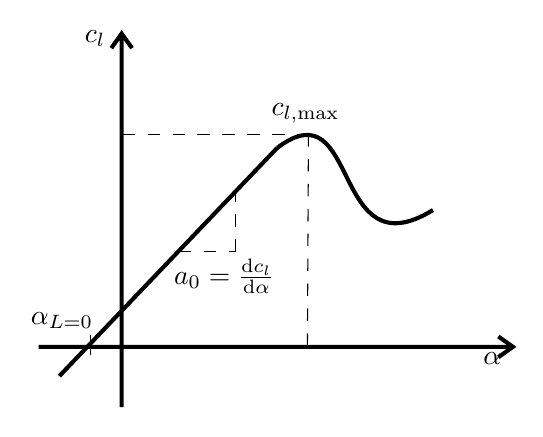
\begin{tikzpicture}[x=0.75pt,y=0.75pt,yscale=-1,xscale=1]
%uncomment if require: \path (0,300); %set diagram left start at 0, and has height of 300

%Shape: Axis 2D [id:dp7499793159263701] 
\draw [line width=1.5]  (200,200.91) -- (428.51,200.91)(240.01,50) -- (240.01,230) (421.51,195.91) -- (428.51,200.91) -- (421.51,205.91) (235.01,57) -- (240.01,50) -- (245.01,57)  ;
%Straight Lines [id:da6818952166992882] 
\draw [line width=1.5]    (315,105) -- (210,215) ;
%Curve Lines [id:da1326114333246986] 
\draw [line width=1.5]    (315,105) .. controls (355,75) and (340.51,165.41) .. (390,135) ;
%Straight Lines [id:da5229353245143065] 
\draw  [dash pattern={on 4.5pt off 4.5pt}]  (240.51,98.41) -- (330.01,98.41) ;
%Straight Lines [id:da4476710750224884] 
\draw  [dash pattern={on 4.5pt off 4.5pt}]  (330.01,98.41) -- (329.51,200.91) ;
%Straight Lines [id:da9636430686615973] 
\draw  [dash pattern={on 4.5pt off 4.5pt}]  (295,125) -- (295,155) ;
%Straight Lines [id:da07371078021099309] 
\draw  [dash pattern={on 4.5pt off 4.5pt}]  (267.51,155) -- (295,155) ;
%Straight Lines [id:da6656415726077622] 
\draw    (225,195) -- (225,205) ;

% Text Node
\draw (221,47.4) node [anchor=north west][inner sep=0.75pt]    {$c_{l}$};
% Text Node
\draw (413,202.4) node [anchor=north west][inner sep=0.75pt]    {$\alpha $};
% Text Node
\draw (195,183) node [anchor=north west][inner sep=0.75pt]    {$\alpha _{L=0}$};
% Text Node
\draw (311,82.4) node [anchor=north west][inner sep=0.75pt]    {$c_{l,\max}$};
% Text Node
\draw (264,157.4) node [anchor=north west][inner sep=0.75pt]    {$a_0=\frac{\mathrm{d}c_l}{\mathrm{d}\alpha}$};


\end{tikzpicture}

	\caption{攻角升力系数曲线}
	\label{fig:angle_of_attack}
\end{figure}

典型的升力系数和攻角之间的变化关系如图\ref{fig:angle_of_attack}所示。
在小攻角和中等攻角的情况下,升力系数随攻角线性变化,这条直线的斜率
记作$a_0$,称为{\bfseries 升力曲线斜率(lift slope)}。在这个区域,空气
从平滑的沿着机翼表面的大部分地方流过。如下图\ref{fig:separate}中左图所示。
\begin{figure}[!ht]
	\centering
	% ! TEX root = ./Incompressible_Flow_over_Airfoils.tex
\tikzset{every picture/.style={line width=0.75pt}} %set default line width to 0.75pt        

\begin{tikzpicture}[x=0.75pt,y=0.75pt,yscale=-1,xscale=1]
%uncomment if require: \path (0,300); %set diagram left start at 0, and has height of 300

%Curve Lines [id:da02066410406444219] 
\draw    (100,121) .. controls (101.51,78.41) and (209.51,108.41) .. (240,120) ;
%Curve Lines [id:da2219924451238391] 
\draw    (380,121) .. controls (381.51,78.41) and (489.51,108.41) .. (520,120) ;
%Curve Lines [id:da14090609932613707] 
\draw    (100,121) .. controls (95.51,131.41) and (187.51,133.41) .. (240,120) ;
%Curve Lines [id:da27960053041213895] 
\draw    (380,121) .. controls (375.51,131.41) and (467.51,133.41) .. (520,120) ;
%Curve Lines [id:da6913211374271631] 
\draw    (80,120) .. controls (106.51,75.41) and (182.51,86.41) .. (240,110) ;
%Curve Lines [id:da7622723644251566] 
\draw    (10,130) .. controls (22.51,129.41) and (59.51,141.41) .. (80,120) ;
%Curve Lines [id:da9760332704223047] 
\draw    (10,150) .. controls (50.51,146.41) and (60,151) .. (100,121) ;
%Curve Lines [id:da5482952107644146] 
\draw    (100,140) .. controls (124.51,140.41) and (190.51,142.41) .. (240,130) ;
%Curve Lines [id:da5631950688908602] 
\draw    (10,170) .. controls (48.51,161.41) and (84.51,139.41) .. (100,140) ;
%Curve Lines [id:da7172273345993287] 
\draw    (360,100) .. controls (395.51,65.41) and (464.51,48.41) .. (520,70) ;
%Curve Lines [id:da6932200849907699] 
\draw    (300,120) .. controls (307.51,117.41) and (327.51,126.41) .. (360,100) ;
%Curve Lines [id:da20447554639464416] 
\draw    (360,130) .. controls (393.51,145.41) and (479.51,143.41) .. (520,130) ;
%Curve Lines [id:da7880084900812823] 
\draw    (300,140) .. controls (309.51,141.41) and (342.51,121.41) .. (360,130) ;
%Curve Lines [id:da0023191113925786766] 
\draw    (470,80) .. controls (462.73,110.47) and (515.2,91.63) .. (492.34,71.84) ;
\draw [shift={(490,70)}, rotate = 35.61] [fill={rgb, 255:red, 0; green, 0; blue, 0 }  ][line width=0.08]  [draw opacity=0] (8.93,-4.29) -- (0,0) -- (8.93,4.29) -- cycle    ;
%Straight Lines [id:da8089051209711549] 
\draw    (150,90) -- (157,90) ;
\draw [shift={(160,90)}, rotate = 180] [fill={rgb, 255:red, 0; green, 0; blue, 0 }  ][line width=0.08]  [draw opacity=0] (8.93,-4.29) -- (0,0) -- (8.93,4.29) -- cycle    ;
%Straight Lines [id:da08051498630628573] 
\draw    (140,140) -- (147,140) ;
\draw [shift={(150,140)}, rotate = 180] [fill={rgb, 255:red, 0; green, 0; blue, 0 }  ][line width=0.08]  [draw opacity=0] (8.93,-4.29) -- (0,0) -- (8.93,4.29) -- cycle    ;
%Straight Lines [id:da1179192395045412] 
\draw    (460,60) -- (467,60) ;
\draw [shift={(470,60)}, rotate = 180] [fill={rgb, 255:red, 0; green, 0; blue, 0 }  ][line width=0.08]  [draw opacity=0] (8.93,-4.29) -- (0,0) -- (8.93,4.29) -- cycle    ;
%Straight Lines [id:da7900053116720815] 
\draw    (440,140) -- (447,140) ;
\draw [shift={(450,140)}, rotate = 180] [fill={rgb, 255:red, 0; green, 0; blue, 0 }  ][line width=0.08]  [draw opacity=0] (8.93,-4.29) -- (0,0) -- (8.93,4.29) -- cycle    ;
%Straight Lines [id:da6440041036552087] 
\draw    (380,50) -- (448.16,79.21) ;
\draw [shift={(450,80)}, rotate = 203.2] [color={rgb, 255:red, 0; green, 0; blue, 0 }  ][line width=0.75]    (10.93,-3.29) .. controls (6.95,-1.4) and (3.31,-0.3) .. (0,0) .. controls (3.31,0.3) and (6.95,1.4) .. (10.93,3.29)   ;

% Text Node
\draw (122,152) node [anchor=north west][inner sep=0.75pt]   [align=left] {小攻角时气流未分离};
% Text Node
\draw (417,151) node [anchor=north west][inner sep=0.75pt]   [align=left] {大攻角下气流分离};
% Text Node
\draw (347,32) node [anchor=north west][inner sep=0.75pt]   [align=left] {分离区域};
% Text Node
\draw (540,112) node [anchor=north west][inner sep=0.75pt]   [align=left] {dead air};


\end{tikzpicture}

	\caption{攻角大小不同时气流流过机翼的流场}
	\label{fig:separate}
\end{figure}
然而,当攻角逐渐变大到一定值时,气流有从翼型上表面分离的趋势,在
机翼后面产生一片“死区空气”(dead air),如图\ref{fig:separate}右图所示。
在气流分离的区域,流动时再循环的。并且有部分流动是与自由来流的方向相
反的,这就是{\bfseries 逆流(reversed flow)}。流动分离主要是因为流体的
粘性效应。
在大攻角下流动分离引起的后果就是{\color{noteorange}升力急剧
减小,阻力急剧增加},这种情况就叫做{\bfseries 失速(stalled)}。

\begin{notice}
	关于流体分离的原文:

	This separated flow is due to
	viscous effects。
\end{notice}
在失速之前,$c_l$的最大值记作$c_{l,\max}$。这是衡量一款翼型的重要指标,
因为它决定了飞机发生失速时的速度。

为了安全起见,把$c_{l \max}$对应的飞行迎角定义为失速迎角,
而不是飞机失速时实际稍高的极限迎角。
\begin{notice}
	$c_{l,\max}$越大,失速速度就越小。
\end{notice}
回到图\ref{fig:angle_of_attack}中,$c_l$随着攻角的增大线性增加,
直到流动分离开始产生影响。然后,曲线开始变成非线性的,$c_l$达到
最大值,最终机翼发生失速。在曲线的另一端,在$\alpha=0$时,升力
是有限的。事实上,只有当飞机低头使得攻角是负的时候,升力才会减小到0。
当升力等于0时的攻角大小叫作{\bfseries 零升攻角(zero-lift angle of attack)},
记作$\alpha_{L=0}$。
\begin{notice}
	对于对称翼型,$\alpha_{L=0}=0$。但是对于大部分有着正弯度的翼型来说,
	$\alpha_{L=0}$是一个负值,一般是$-2$或$-3^{\circ}$的数量级。
\end{notice}

实验表明,升力曲线的斜率不受雷诺数影响,但是$c_{l,\max}$取决于
雷诺数。
\begin{notice}
	因为$c_{l,\max}$被粘性控制,并且雷诺数是一个相似参数,
	它决定了流动中惯性力和粘性力的比值。
\end{notice}

翼型的气动力矩是攻角的函数,但是在翼型上存在一个点,使得气动
力矩的大小和攻角无关,这个点叫做{\bfseries 空气动力中心(aerodynamic center)}。
这个点一般位于距机翼前缘$\frac{c}{4}$的位置。
\begin{example}
	给定翼型为NACA 2412,弦长是$0.64$m,在标准海平面上飞行,自由
	来流的速度是$70$m/s,单位翼展上的升力是$1254$N/m。计算飞行迎角
	和单位翼展上的阻力大小。


	在标准海平面上,$\rho=1.23\text{Kg/m}^3$:
	\[
		q_\infty =\frac{1}{2}\rho_\infty V_\infty ^2 =\frac{1}{2}\times 1.23\times 70^2=3013.5
		\text{N/m}^2
	\]
	\[
		c_l=\frac{L}{q_\infty S}=\frac{L}{q_\infty c}=\frac{1254}{3013.3\times 0.64}=0.65
	\]
	对于$c_l=0.65$,查升力曲线图,得到$\alpha=4^\circ$。

	标准海平面上,$\mu=1.789\times 10^{-5}\text{Kg/m$\cdot$ s}$:
	\[
		\mathrm{Re}=\frac{\rho_\infty V_\infty c }{\mu_\infty}=\frac{14.23\times 70\times 0.64}{1.789\times 10^{-5}}
		=3.08\times 10^6
	\]
	查阻力曲线图,得到$c_d=0.0068$,因此
	\[
		D=q_\infty S c_d=q_\infty c c_d=3013.5\times 0.64\times 0.0068=13.1\text{N/m}
	\]
\end{example}
\begin{example}
	对于NACA 2412翼型,计算并比较攻角分别在$0^\circ$,$4^\circ$,$8^\circ$,$12^\circ$
	时的升阻比,雷诺数是$3.1\times 10^6$。

	查升力曲线图和阻力曲线图得到下表

	\centering
	\begin{tabular}{llll}
		\toprule
		$\alpha$ & $c_l$ & $c_d$  & $c_l /c_d$ \\
		\midrule
		0        & 0.25  & 0.0065 & 38.5       \\
		4        & 0.65  & 0.0070 & 93         \\
		8        & 1.08  & 0.0112 & 96         \\
		12       & 1.44  & 0.017  & 85         \\
		\bottomrule
	\end{tabular}
\end{example}

从上面例题可以看出,随着攻角增大,升阻比先增大,
达到一个最大值,然后减小。升阻比的最大值是翼型
性能的一个重要参数。它能直接表明翼型的效率。
{\color{noteorange}升阻比越大,翼型的效率就越高}。
由于飞机其他部分的阻力,实际飞机的升阻比一般在10到
20这样的量级。

\section{用于低速流动下的机翼的理论解法:面涡}
想象一根直线垂直于纸面,通过一个点$O$,并且向
纸面的里面和外面无限延伸。这条直线就是强度为
$\Gamma$的{\bfseries 涡旋线(vortex filament)}。
通过这根涡旋线在任意垂直于这个涡旋线的平面上
诱导出的流场和强度为$\Gamma$的点涡诱导出的流
场是一样的。事实上,可以将涡旋线看成是无数点
涡组成的。

对于一个涡流场,考虑和面源相似的情况。想象
无数根涡旋线紧挨着,这些涡旋线的强度又是无穷小。
这些涡旋线就形成了一个{\bfseries 面涡(vortex sheet)}。
顺着这些涡旋线看去,面涡就会变成如图\ref{fig:vortex sheet}
所示的场景。
\begin{figure}[!ht]
  \centering
  % ! TEX root = ./Incompressible_Flow_over_Airfoils.tex

\tikzset{every picture/.style={line width=0.75pt}} %set default line width to 0.75pt        

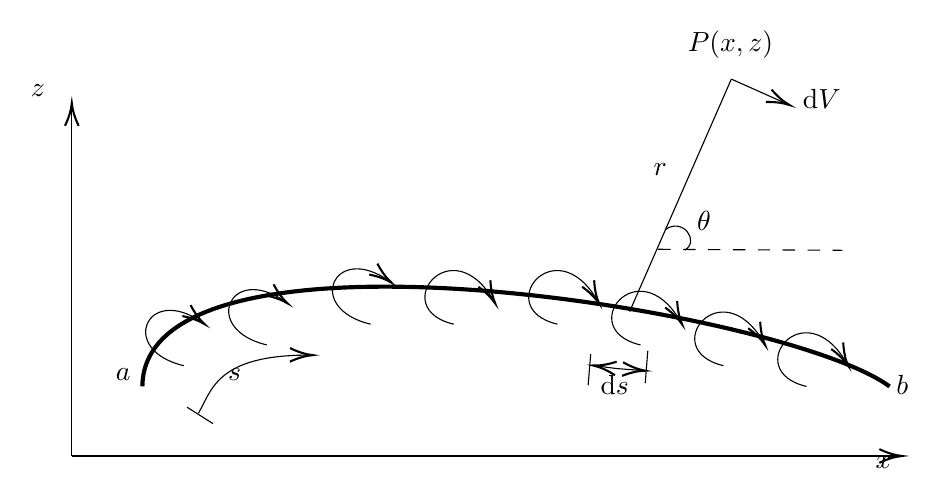
\begin{tikzpicture}[x=0.75pt,y=0.75pt,yscale=-1,xscale=1]
%uncomment if require: \path (0,285); %set diagram left start at 0, and has height of 285

%Curve Lines [id:da8763652678817189] 
\draw [line width=1.5]    (104,206.5) .. controls (104.51,119.91) and (414,169.5) .. (464,206.5) ;
%Curve Lines [id:da4750021580535706] 
\draw    (124,196.5) .. controls (92,189.03) and (106.07,156.9) .. (132.77,175.61) ;
\draw [shift={(134,176.5)}, rotate = 216.83] [color={rgb, 255:red, 0; green, 0; blue, 0 }  ][line width=0.75]    (10.93,-3.29) .. controls (6.95,-1.4) and (3.31,-0.3) .. (0,0) .. controls (3.31,0.3) and (6.95,1.4) .. (10.93,3.29)   ;
%Curve Lines [id:da2895808384347458] 
\draw    (164,186.5) .. controls (132,179.03) and (146.07,146.9) .. (172.77,165.61) ;
\draw [shift={(174,166.5)}, rotate = 216.83] [color={rgb, 255:red, 0; green, 0; blue, 0 }  ][line width=0.75]    (10.93,-3.29) .. controls (6.95,-1.4) and (3.31,-0.3) .. (0,0) .. controls (3.31,0.3) and (6.95,1.4) .. (10.93,3.29)   ;
%Curve Lines [id:da7153231460572151] 
\draw    (214,176.5) .. controls (182,169.03) and (196.07,136.9) .. (222.77,155.61) ;
\draw [shift={(224,156.5)}, rotate = 216.83] [color={rgb, 255:red, 0; green, 0; blue, 0 }  ][line width=0.75]    (10.93,-3.29) .. controls (6.95,-1.4) and (3.31,-0.3) .. (0,0) .. controls (3.31,0.3) and (6.95,1.4) .. (10.93,3.29)   ;
%Curve Lines [id:da9877697377632966] 
\draw    (254,176.5) .. controls (222,169.03) and (252.56,130.11) .. (273.07,164.86) ;
\draw [shift={(274,166.5)}, rotate = 241.4] [color={rgb, 255:red, 0; green, 0; blue, 0 }  ][line width=0.75]    (10.93,-3.29) .. controls (6.95,-1.4) and (3.31,-0.3) .. (0,0) .. controls (3.31,0.3) and (6.95,1.4) .. (10.93,3.29)   ;
%Curve Lines [id:da6202187083118886] 
\draw    (304,176.5) .. controls (272,169.03) and (302.56,130.11) .. (323.07,164.86) ;
\draw [shift={(324,166.5)}, rotate = 241.4] [color={rgb, 255:red, 0; green, 0; blue, 0 }  ][line width=0.75]    (10.93,-3.29) .. controls (6.95,-1.4) and (3.31,-0.3) .. (0,0) .. controls (3.31,0.3) and (6.95,1.4) .. (10.93,3.29)   ;
%Curve Lines [id:da8336758488674814] 
\draw    (344,186.5) .. controls (312,179.03) and (342.56,140.11) .. (363.07,174.86) ;
\draw [shift={(364,176.5)}, rotate = 241.4] [color={rgb, 255:red, 0; green, 0; blue, 0 }  ][line width=0.75]    (10.93,-3.29) .. controls (6.95,-1.4) and (3.31,-0.3) .. (0,0) .. controls (3.31,0.3) and (6.95,1.4) .. (10.93,3.29)   ;
%Curve Lines [id:da8897778956265143] 
\draw    (384,196.5) .. controls (352,189.03) and (382.56,150.11) .. (403.07,184.86) ;
\draw [shift={(404,186.5)}, rotate = 241.4] [color={rgb, 255:red, 0; green, 0; blue, 0 }  ][line width=0.75]    (10.93,-3.29) .. controls (6.95,-1.4) and (3.31,-0.3) .. (0,0) .. controls (3.31,0.3) and (6.95,1.4) .. (10.93,3.29)   ;
%Curve Lines [id:da04487167241342771] 
\draw    (424,206.5) .. controls (392,199.03) and (422.56,160.11) .. (443.07,194.86) ;
\draw [shift={(444,196.5)}, rotate = 241.4] [color={rgb, 255:red, 0; green, 0; blue, 0 }  ][line width=0.75]    (10.93,-3.29) .. controls (6.95,-1.4) and (3.31,-0.3) .. (0,0) .. controls (3.31,0.3) and (6.95,1.4) .. (10.93,3.29)   ;
%Straight Lines [id:da5621055060339388] 
\draw    (125.5,216.5) -- (138.01,224.41) ;
%Curve Lines [id:da3596797142445818] 
\draw    (131.01,219.41) .. controls (137.45,208.52) and (139.47,191.26) .. (184.63,191.4) ;
\draw [shift={(186.01,191.41)}, rotate = 180.62] [color={rgb, 255:red, 0; green, 0; blue, 0 }  ][line width=0.75]    (10.93,-3.29) .. controls (6.95,-1.4) and (3.31,-0.3) .. (0,0) .. controls (3.31,0.3) and (6.95,1.4) .. (10.93,3.29)   ;
%Straight Lines [id:da4909959828720716] 
\draw    (347.5,189.41) -- (346.26,204.91) ;
%Straight Lines [id:da5091055511160192] 
\draw    (318.76,205.91) -- (320,190.91) ;
%Straight Lines [id:da5213093595184453] 
\draw    (332.76,197.91) -- (344.27,198.77) ;
\draw [shift={(346.26,198.91)}, rotate = 184.24] [color={rgb, 255:red, 0; green, 0; blue, 0 }  ][line width=0.75]    (10.93,-3.29) .. controls (6.95,-1.4) and (3.31,-0.3) .. (0,0) .. controls (3.31,0.3) and (6.95,1.4) .. (10.93,3.29)   ;
%Straight Lines [id:da04498336011734372] 
\draw    (332.76,197.91) -- (323.24,196.67) ;
\draw [shift={(321.26,196.41)}, rotate = 7.43] [color={rgb, 255:red, 0; green, 0; blue, 0 }  ][line width=0.75]    (10.93,-3.29) .. controls (6.95,-1.4) and (3.31,-0.3) .. (0,0) .. controls (3.31,0.3) and (6.95,1.4) .. (10.93,3.29)   ;
%Straight Lines [id:da31365051851853876] 
\draw    (338.76,170.41) -- (387.76,58.41) ;
%Straight Lines [id:da29570303575193213] 
\draw  [dash pattern={on 4.5pt off 4.5pt}]  (352.5,140.41) -- (368.26,140.5) -- (441.26,140.91) ;
%Curve Lines [id:da3186708293732772] 
\draw    (356,130.91) .. controls (364.26,124.91) and (372.76,136.41) .. (365.26,140.91) ;
%Straight Lines [id:da09450810625839368] 
\draw    (387.76,58.41) -- (413.94,70.1) ;
\draw [shift={(415.76,70.91)}, rotate = 204.06] [color={rgb, 255:red, 0; green, 0; blue, 0 }  ][line width=0.75]    (10.93,-3.29) .. controls (6.95,-1.4) and (3.31,-0.3) .. (0,0) .. controls (3.31,0.3) and (6.95,1.4) .. (10.93,3.29)   ;
%Straight Lines [id:da5222357770732207] 
\draw    (70,240) -- (70,72) ;
\draw [shift={(70,70)}, rotate = 90] [color={rgb, 255:red, 0; green, 0; blue, 0 }  ][line width=0.75]    (10.93,-3.29) .. controls (6.95,-1.4) and (3.31,-0.3) .. (0,0) .. controls (3.31,0.3) and (6.95,1.4) .. (10.93,3.29)   ;
%Straight Lines [id:da5641055148269973] 
\draw    (70,240) -- (468,240) ;
\draw [shift={(470,240)}, rotate = 180] [color={rgb, 255:red, 0; green, 0; blue, 0 }  ][line width=0.75]    (10.93,-3.29) .. controls (6.95,-1.4) and (3.31,-0.3) .. (0,0) .. controls (3.31,0.3) and (6.95,1.4) .. (10.93,3.29)   ;

% Text Node
\draw (90,196.5) node [anchor=north west][inner sep=0.75pt]    {$a$};
% Text Node
\draw (144,196.5) node [anchor=north west][inner sep=0.75pt]    {$s$};
% Text Node
\draw (466,200) node [anchor=north west][inner sep=0.75pt]    {$b$};
% Text Node
\draw (323.5,199.91) node [anchor=north west][inner sep=0.75pt]    {$\mathrm{d}s$};
% Text Node
\draw (349,97.91) node [anchor=north west][inner sep=0.75pt]    {$r$};
% Text Node
\draw (370,120.91) node [anchor=north west][inner sep=0.75pt]    {$\theta $};
% Text Node
\draw (365.5,33.91) node [anchor=north west][inner sep=0.75pt]    {$P(x,z)$};
% Text Node
\draw (421,61.91) node [anchor=north west][inner sep=0.75pt]    {$\mathrm{d}V$};
% Text Node
\draw (49,60) node [anchor=north west][inner sep=0.75pt]    {$z$};
% Text Node
\draw (456,239) node [anchor=north west][inner sep=0.75pt]    {$x$};


\end{tikzpicture}

  \caption{面涡的边缘视角}
  \label{fig:vortex sheet}
\end{figure}
所有的涡旋线都垂直于纸面。设$s$是沿着面涡边缘
视角下的距离坐标。定义$\gamma=\gamma(s)$是
坐标为$s$的单位长度上面涡的强度。因此,对于
无限小长度$\mathrm{d}s$上的面涡强度就是
$\gamma\mathrm{d}s$。面涡的这一小部分
可以看成是强度为$\gamma\mathrm{d}s $的点涡。
现在考虑位于流场中的一个点$P$,和$\mathrm{d}s$的距离
是$r$;坐标是$(x,z)$。强度为$\gamma\mathrm{d}s$的
面涡在$P$点诱导出无穷小的速度$\mathrm{d}V$,即
\[
  \mathrm{d}V=-\frac{\gamma \mathrm{d}s }{2\pi r }
\]
并且方向垂直于$r$。$P$点的诱导速度就是整个面涡从
$a$点到$b$点上式的总和。不同面涡部分在$P$点产生的
速度的叠加必须是矢量叠加的。由于这个,使得处理速度势
就更方便了。通过单元涡$\gamma \mathrm{d}s $在$P$点
诱导出的速度势$\mathrm{d} \Phi$的增量就是
\[
  \mathrm{d}\Phi=-\frac{\gamma \mathrm{d}s }{2\pi}\theta
\]
相应的,从$a$到$b $整个面涡在$P$点的速度势就是
\[
  \Phi(x,z)=- \frac{1}{2\pi}\int _a^b \theta \gamma \mathrm{d}s 
\]
上面这个方程对于薄翼理论的讨论是特别有用的,同时对于涡面元的
数值解法也是特别重要的。

一个点涡的环量$\Gamma$等于这个涡的强度。在图\ref{fig:vortex sheet}
中面涡的环量就是这些涡单元的强度的总和;即
\[
  \Gamma=\int _a^b \gamma \mathrm{d}s 
\]

面源的法向速度分量是不连续的,而速度的切向分量在
面源的上方和下方是一样的。与面源恰恰相反,面涡的切向
速度分量是不连续的,而法向速度分量是连续的。速度的
切向分量的变化大小和面涡的强度是有关系的。考虑一个面涡
如下图\ref{fig:strength_vortex}所示,
\begin{figure}[!ht]
  \centering
  % !TEX root = ./Incompressible_Flow_over_Airfoils.tex

\tikzset{every picture/.style={line width=0.75pt}} %set default line width to 0.75pt        

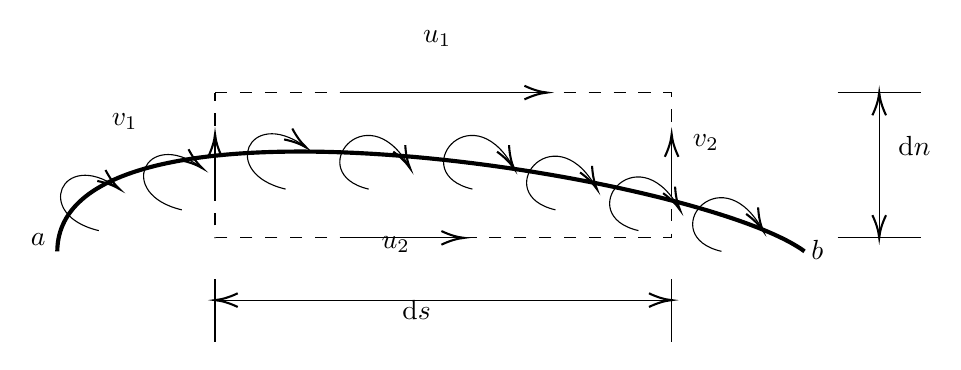
\begin{tikzpicture}[x=0.75pt,y=0.75pt,yscale=-1,xscale=1]
%uncomment if require: \path (0,285); %set diagram left start at 0, and has height of 285

%Curve Lines [id:da8763652678817189] 
\draw [line width=1.5]    (104,206.5) .. controls (104.51,119.91) and (414,169.5) .. (464,206.5) ;
%Curve Lines [id:da4750021580535706] 
\draw    (124,196.5) .. controls (92,189.03) and (106.07,156.9) .. (132.77,175.61) ;
\draw [shift={(134,176.5)}, rotate = 216.83] [color={rgb, 255:red, 0; green, 0; blue, 0 }  ][line width=0.75]    (10.93,-3.29) .. controls (6.95,-1.4) and (3.31,-0.3) .. (0,0) .. controls (3.31,0.3) and (6.95,1.4) .. (10.93,3.29)   ;
%Curve Lines [id:da2895808384347458] 
\draw    (164,186.5) .. controls (132,179.03) and (146.07,146.9) .. (172.77,165.61) ;
\draw [shift={(174,166.5)}, rotate = 216.83] [color={rgb, 255:red, 0; green, 0; blue, 0 }  ][line width=0.75]    (10.93,-3.29) .. controls (6.95,-1.4) and (3.31,-0.3) .. (0,0) .. controls (3.31,0.3) and (6.95,1.4) .. (10.93,3.29)   ;
%Curve Lines [id:da7153231460572151] 
\draw    (214,176.5) .. controls (182,169.03) and (196.07,136.9) .. (222.77,155.61) ;
\draw [shift={(224,156.5)}, rotate = 216.83] [color={rgb, 255:red, 0; green, 0; blue, 0 }  ][line width=0.75]    (10.93,-3.29) .. controls (6.95,-1.4) and (3.31,-0.3) .. (0,0) .. controls (3.31,0.3) and (6.95,1.4) .. (10.93,3.29)   ;
%Curve Lines [id:da9877697377632966] 
\draw    (254,176.5) .. controls (222,169.03) and (252.56,130.11) .. (273.07,164.86) ;
\draw [shift={(274,166.5)}, rotate = 241.4] [color={rgb, 255:red, 0; green, 0; blue, 0 }  ][line width=0.75]    (10.93,-3.29) .. controls (6.95,-1.4) and (3.31,-0.3) .. (0,0) .. controls (3.31,0.3) and (6.95,1.4) .. (10.93,3.29)   ;
%Curve Lines [id:da6202187083118886] 
\draw    (304,176.5) .. controls (272,169.03) and (302.56,130.11) .. (323.07,164.86) ;
\draw [shift={(324,166.5)}, rotate = 241.4] [color={rgb, 255:red, 0; green, 0; blue, 0 }  ][line width=0.75]    (10.93,-3.29) .. controls (6.95,-1.4) and (3.31,-0.3) .. (0,0) .. controls (3.31,0.3) and (6.95,1.4) .. (10.93,3.29)   ;
%Curve Lines [id:da8336758488674814] 
\draw    (344,186.5) .. controls (312,179.03) and (342.56,140.11) .. (363.07,174.86) ;
\draw [shift={(364,176.5)}, rotate = 241.4] [color={rgb, 255:red, 0; green, 0; blue, 0 }  ][line width=0.75]    (10.93,-3.29) .. controls (6.95,-1.4) and (3.31,-0.3) .. (0,0) .. controls (3.31,0.3) and (6.95,1.4) .. (10.93,3.29)   ;
%Curve Lines [id:da8897778956265143] 
\draw    (384,196.5) .. controls (352,189.03) and (382.56,150.11) .. (403.07,184.86) ;
\draw [shift={(404,186.5)}, rotate = 241.4] [color={rgb, 255:red, 0; green, 0; blue, 0 }  ][line width=0.75]    (10.93,-3.29) .. controls (6.95,-1.4) and (3.31,-0.3) .. (0,0) .. controls (3.31,0.3) and (6.95,1.4) .. (10.93,3.29)   ;
%Curve Lines [id:da04487167241342771] 
\draw    (424,206.5) .. controls (392,199.03) and (422.56,160.11) .. (443.07,194.86) ;
\draw [shift={(444,196.5)}, rotate = 241.4] [color={rgb, 255:red, 0; green, 0; blue, 0 }  ][line width=0.75]    (10.93,-3.29) .. controls (6.95,-1.4) and (3.31,-0.3) .. (0,0) .. controls (3.31,0.3) and (6.95,1.4) .. (10.93,3.29)   ;
%Shape: Rectangle [id:dp15963879701718064] 
\draw  [dash pattern={on 4.5pt off 4.5pt}] (180,130) -- (400,130) -- (400,200) -- (180,200) -- cycle ;
%Straight Lines [id:da8026280446997687] 
\draw    (240,130) -- (338,130) ;
\draw [shift={(340,130)}, rotate = 180] [color={rgb, 255:red, 0; green, 0; blue, 0 }  ][line width=0.75]    (10.93,-3.29) .. controls (6.95,-1.4) and (3.31,-0.3) .. (0,0) .. controls (3.31,0.3) and (6.95,1.4) .. (10.93,3.29)   ;
%Straight Lines [id:da3245350317643181] 
\draw    (240,200) -- (298,200) ;
\draw [shift={(300,200)}, rotate = 180] [color={rgb, 255:red, 0; green, 0; blue, 0 }  ][line width=0.75]    (10.93,-3.29) .. controls (6.95,-1.4) and (3.31,-0.3) .. (0,0) .. controls (3.31,0.3) and (6.95,1.4) .. (10.93,3.29)   ;
%Straight Lines [id:da7628086801385121] 
\draw    (180,180) -- (180,152) ;
\draw [shift={(180,150)}, rotate = 90] [color={rgb, 255:red, 0; green, 0; blue, 0 }  ][line width=0.75]    (10.93,-3.29) .. controls (6.95,-1.4) and (3.31,-0.3) .. (0,0) .. controls (3.31,0.3) and (6.95,1.4) .. (10.93,3.29)   ;
%Straight Lines [id:da347003095117139] 
\draw    (400,180) -- (400,152) ;
\draw [shift={(400,150)}, rotate = 90] [color={rgb, 255:red, 0; green, 0; blue, 0 }  ][line width=0.75]    (10.93,-3.29) .. controls (6.95,-1.4) and (3.31,-0.3) .. (0,0) .. controls (3.31,0.3) and (6.95,1.4) .. (10.93,3.29)   ;
%Straight Lines [id:da6243635216764141] 
\draw    (180,220) -- (180,250) ;
%Straight Lines [id:da6817985927803263] 
\draw    (400,220) -- (400,250) ;
%Straight Lines [id:da9105574441608693] 
\draw    (290,230) -- (398,230) ;
\draw [shift={(400,230)}, rotate = 180] [color={rgb, 255:red, 0; green, 0; blue, 0 }  ][line width=0.75]    (10.93,-3.29) .. controls (6.95,-1.4) and (3.31,-0.3) .. (0,0) .. controls (3.31,0.3) and (6.95,1.4) .. (10.93,3.29)   ;
%Straight Lines [id:da7767579818993569] 
\draw    (290,230) -- (182,230) ;
\draw [shift={(180,230)}, rotate = 360] [color={rgb, 255:red, 0; green, 0; blue, 0 }  ][line width=0.75]    (10.93,-3.29) .. controls (6.95,-1.4) and (3.31,-0.3) .. (0,0) .. controls (3.31,0.3) and (6.95,1.4) .. (10.93,3.29)   ;
%Straight Lines [id:da3361994371134467] 
\draw    (480,200) -- (520,200) ;
%Straight Lines [id:da04570162822709278] 
\draw    (480,130) -- (520,130) ;
%Straight Lines [id:da6631521119255424] 
\draw    (500,160) -- (500,198) ;
\draw [shift={(500,200)}, rotate = 270] [color={rgb, 255:red, 0; green, 0; blue, 0 }  ][line width=0.75]    (10.93,-3.29) .. controls (6.95,-1.4) and (3.31,-0.3) .. (0,0) .. controls (3.31,0.3) and (6.95,1.4) .. (10.93,3.29)   ;
%Straight Lines [id:da14321333492030197] 
\draw    (500,160) -- (500,132) ;
\draw [shift={(500,130)}, rotate = 90] [color={rgb, 255:red, 0; green, 0; blue, 0 }  ][line width=0.75]    (10.93,-3.29) .. controls (6.95,-1.4) and (3.31,-0.3) .. (0,0) .. controls (3.31,0.3) and (6.95,1.4) .. (10.93,3.29)   ;

% Text Node
\draw (90,196.5) node [anchor=north west][inner sep=0.75pt]    {$a$};
% Text Node
\draw (466,200) node [anchor=north west][inner sep=0.75pt]    {$b$};
% Text Node
\draw (279,99) node [anchor=north west][inner sep=0.75pt]    {$u_{1}$};
% Text Node
\draw (259,198) node [anchor=north west][inner sep=0.75pt]    {$u_{2}$};
% Text Node
\draw (129,139) node [anchor=north west][inner sep=0.75pt]    {$v_{1}$};
% Text Node
\draw (409,149) node [anchor=north west][inner sep=0.75pt]    {$v_{2}$};
% Text Node
\draw (269,229) node [anchor=north west][inner sep=0.75pt]    {$\mathrm{d}s$};
% Text Node
\draw (508,150) node [anchor=north west][inner sep=0.75pt]    {$\mathrm{d}n$};


\end{tikzpicture}

  \caption{面涡切向分量的跳跃}
  \label{fig:strength_vortex}
\end{figure}
使用一个虚线的矩形框包围一部分面涡,长度是$\mathrm{d}s $。
速度在上下的切向分量分别是$u_1$和$u_2$,左右两边的切向
分量分别是$v_1$和$v_2$,上下两边的距离是$\mathrm{d}n $。
从环量的定义,可以得到这个虚线框的环量是
\[
  \Gamma=-(v_2 \mathrm{d}n -u_1 \mathrm{d}s -v_1 \mathrm{d}n +u_2 \mathrm{d}s)
\]
或
\[
  \Gamma= (u_1-u_2) \mathrm{d}s+(v_1-v_2) \mathrm{d}n
\]
然而,因为包围在虚线路径中的面涡的强度是$\gamma \mathrm{d}s $,于是
\[
  \Gamma =\gamma \mathrm{d}s 
\]
因此
\[
  \gamma \mathrm{d} s =(u_1-u_2 )\mathrm{d}s+(v_1-v_2) \mathrm{d}n
\]
现在让上下表面靠近面涡,即$\mathrm{d}n \rightarrow 0$。在
极限情况下,$u_1$和$u_2$就迅速称为面涡上下表面的切向速度,
上式就可以写成
\[
  \gamma \mathrm{d}s =(u_1-u_2)\mathrm{d}s 
\]
或者
\[
  \gamma =u_1-u_2
\]
这个等式非常重要。它表明了{\bfseries 当地面涡切向速度跳跃的差值
就等于当地面涡的强度}。

面涡的概念是在低速翼型性质分析中的一个工具。考虑在自由来流的速度
为$V_\infty$中的有着任意形状和厚度的翼型,如图\ref{fig:distributing}
\begin{figure}[!ht]
  \centering
  % ! TEX root = ./Incompressible_Flow_over_Airfoils.tex

\tikzset{every picture/.style={line width=0.75pt}} %set default line width to 0.75pt        

\begin{tikzpicture}[x=0.75pt,y=0.75pt,yscale=-1,xscale=1]
%uncomment if require: \path (0,285); %set diagram left start at 0, and has height of 285

%Curve Lines [id:da8763652678817189] 
\draw [line width=1.5]    (180,206.5) .. controls (180.51,119.91) and (490,169.5) .. (540,206.5) ;
%Curve Lines [id:da4750021580535706] 
\draw    (200,196.5) .. controls (168,189.03) and (182.07,156.9) .. (208.77,175.61) ;
\draw [shift={(210,176.5)}, rotate = 216.83] [color={rgb, 255:red, 0; green, 0; blue, 0 }  ][line width=0.75]    (10.93,-3.29) .. controls (6.95,-1.4) and (3.31,-0.3) .. (0,0) .. controls (3.31,0.3) and (6.95,1.4) .. (10.93,3.29)   ;
%Curve Lines [id:da2895808384347458] 
\draw    (240,186.5) .. controls (208,179.03) and (222.07,146.9) .. (248.77,165.61) ;
\draw [shift={(250,166.5)}, rotate = 216.83] [color={rgb, 255:red, 0; green, 0; blue, 0 }  ][line width=0.75]    (10.93,-3.29) .. controls (6.95,-1.4) and (3.31,-0.3) .. (0,0) .. controls (3.31,0.3) and (6.95,1.4) .. (10.93,3.29)   ;
%Curve Lines [id:da7153231460572151] 
\draw    (290,176.5) .. controls (258,169.03) and (272.07,136.9) .. (298.77,155.61) ;
\draw [shift={(300,156.5)}, rotate = 216.83] [color={rgb, 255:red, 0; green, 0; blue, 0 }  ][line width=0.75]    (10.93,-3.29) .. controls (6.95,-1.4) and (3.31,-0.3) .. (0,0) .. controls (3.31,0.3) and (6.95,1.4) .. (10.93,3.29)   ;
%Curve Lines [id:da9877697377632966] 
\draw    (330,176.5) .. controls (298,169.03) and (328.56,130.11) .. (349.07,164.86) ;
\draw [shift={(350,166.5)}, rotate = 241.4] [color={rgb, 255:red, 0; green, 0; blue, 0 }  ][line width=0.75]    (10.93,-3.29) .. controls (6.95,-1.4) and (3.31,-0.3) .. (0,0) .. controls (3.31,0.3) and (6.95,1.4) .. (10.93,3.29)   ;
%Curve Lines [id:da6202187083118886] 
\draw    (380,176.5) .. controls (348,169.03) and (378.56,130.11) .. (399.07,164.86) ;
\draw [shift={(400,166.5)}, rotate = 241.4] [color={rgb, 255:red, 0; green, 0; blue, 0 }  ][line width=0.75]    (10.93,-3.29) .. controls (6.95,-1.4) and (3.31,-0.3) .. (0,0) .. controls (3.31,0.3) and (6.95,1.4) .. (10.93,3.29)   ;
%Curve Lines [id:da8336758488674814] 
\draw    (420,186.5) .. controls (388,179.03) and (418.56,140.11) .. (439.07,174.86) ;
\draw [shift={(440,176.5)}, rotate = 241.4] [color={rgb, 255:red, 0; green, 0; blue, 0 }  ][line width=0.75]    (10.93,-3.29) .. controls (6.95,-1.4) and (3.31,-0.3) .. (0,0) .. controls (3.31,0.3) and (6.95,1.4) .. (10.93,3.29)   ;
%Curve Lines [id:da8897778956265143] 
\draw    (460,196.5) .. controls (428,189.03) and (458.56,150.11) .. (479.07,184.86) ;
\draw [shift={(480,186.5)}, rotate = 241.4] [color={rgb, 255:red, 0; green, 0; blue, 0 }  ][line width=0.75]    (10.93,-3.29) .. controls (6.95,-1.4) and (3.31,-0.3) .. (0,0) .. controls (3.31,0.3) and (6.95,1.4) .. (10.93,3.29)   ;
%Curve Lines [id:da04487167241342771] 
\draw    (500,206.5) .. controls (468,199.03) and (498.56,160.11) .. (519.07,194.86) ;
\draw [shift={(520,196.5)}, rotate = 241.4] [color={rgb, 255:red, 0; green, 0; blue, 0 }  ][line width=0.75]    (10.93,-3.29) .. controls (6.95,-1.4) and (3.31,-0.3) .. (0,0) .. controls (3.31,0.3) and (6.95,1.4) .. (10.93,3.29)   ;
%Curve Lines [id:da7056965185008723] 
\draw [line width=1.5]    (180,206.5) .. controls (191.76,233.66) and (481.26,217.66) .. (540,206.5) ;
%Curve Lines [id:da9786572690593871] 
\draw    (216,230) .. controls (184,222.53) and (198.07,190.4) .. (224.77,209.11) ;
\draw [shift={(226,210)}, rotate = 216.83] [color={rgb, 255:red, 0; green, 0; blue, 0 }  ][line width=0.75]    (10.93,-3.29) .. controls (6.95,-1.4) and (3.31,-0.3) .. (0,0) .. controls (3.31,0.3) and (6.95,1.4) .. (10.93,3.29)   ;
%Curve Lines [id:da7370114979998401] 
\draw    (256,240) .. controls (224,232.53) and (238.07,200.4) .. (264.77,219.11) ;
\draw [shift={(266,220)}, rotate = 216.83] [color={rgb, 255:red, 0; green, 0; blue, 0 }  ][line width=0.75]    (10.93,-3.29) .. controls (6.95,-1.4) and (3.31,-0.3) .. (0,0) .. controls (3.31,0.3) and (6.95,1.4) .. (10.93,3.29)   ;
%Curve Lines [id:da565688073975608] 
\draw    (306,240) .. controls (274,232.53) and (288.07,200.4) .. (314.77,219.11) ;
\draw [shift={(316,220)}, rotate = 216.83] [color={rgb, 255:red, 0; green, 0; blue, 0 }  ][line width=0.75]    (10.93,-3.29) .. controls (6.95,-1.4) and (3.31,-0.3) .. (0,0) .. controls (3.31,0.3) and (6.95,1.4) .. (10.93,3.29)   ;
%Curve Lines [id:da36584632780625626] 
\draw    (356,240) .. controls (324,232.53) and (338.07,200.4) .. (364.77,219.11) ;
\draw [shift={(366,220)}, rotate = 216.83] [color={rgb, 255:red, 0; green, 0; blue, 0 }  ][line width=0.75]    (10.93,-3.29) .. controls (6.95,-1.4) and (3.31,-0.3) .. (0,0) .. controls (3.31,0.3) and (6.95,1.4) .. (10.93,3.29)   ;
%Curve Lines [id:da24575083934992725] 
\draw    (406,240) .. controls (374,232.53) and (388.07,200.4) .. (414.77,219.11) ;
\draw [shift={(416,220)}, rotate = 216.83] [color={rgb, 255:red, 0; green, 0; blue, 0 }  ][line width=0.75]    (10.93,-3.29) .. controls (6.95,-1.4) and (3.31,-0.3) .. (0,0) .. controls (3.31,0.3) and (6.95,1.4) .. (10.93,3.29)   ;
%Curve Lines [id:da6411532602375065] 
\draw    (456,230) .. controls (424,222.53) and (438.07,190.4) .. (464.77,209.11) ;
\draw [shift={(466,210)}, rotate = 216.83] [color={rgb, 255:red, 0; green, 0; blue, 0 }  ][line width=0.75]    (10.93,-3.29) .. controls (6.95,-1.4) and (3.31,-0.3) .. (0,0) .. controls (3.31,0.3) and (6.95,1.4) .. (10.93,3.29)   ;
%Straight Lines [id:da5087801996340116] 
\draw    (30,210) -- (128,210) ;
\draw [shift={(130,210)}, rotate = 180] [color={rgb, 255:red, 0; green, 0; blue, 0 }  ][line width=0.75]    (10.93,-3.29) .. controls (6.95,-1.4) and (3.31,-0.3) .. (0,0) .. controls (3.31,0.3) and (6.95,1.4) .. (10.93,3.29)   ;
%Curve Lines [id:da5329178372398633] 
\draw    (160,200) .. controls (144.17,180.86) and (179.79,141.46) .. (228.52,149.73) ;
\draw [shift={(230,150)}, rotate = 190.68] [color={rgb, 255:red, 0; green, 0; blue, 0 }  ][line width=0.75]    (10.93,-3.29) .. controls (6.95,-1.4) and (3.31,-0.3) .. (0,0) .. controls (3.31,0.3) and (6.95,1.4) .. (10.93,3.29)   ;

% Text Node
\draw (242,189.5) node [anchor=north west][inner sep=0.75pt]   [align=left] {有任意形状和厚度的翼型};
% Text Node
\draw (61,222.4) node [anchor=north west][inner sep=0.75pt]    {$V_{\infty }$};
% Text Node
\draw (158,133.4) node [anchor=north west][inner sep=0.75pt]    {$s$};
% Text Node
\draw (400,132.4) node [anchor=north west][inner sep=0.75pt]    {$\gamma ( s)$};


\end{tikzpicture}

  \caption{任意翼型面涡在表面的分布}
  \label{fig:distributing}
\end{figure}
面涡的强度分布函数就是$\gamma(s)$。计算$\gamma$关于
$s$的函数,当诱导出的速度场加上统一的速度大小为$V_\infty$
后,就会使得面涡(翼型表面)称为流场中的一条流线。
相应的,绕机翼的环量就通过
\[
  \Gamma= \int \gamma \mathrm{d}s 
\]
给出,这个积分是沿着整个机翼表面给出的。
最后,升力通过库塔-茹科夫斯基定理给出
\[
  L'=\rho _\infty V_\infty \Gamma
\]
然而,并没有通用的分析解法给出$\gamma=\gamma(s)$对于
任意厚度和形状的机翼。相反,面涡的强度必须通过
数值的方法求解出。上述解法是{\bfseries 涡流面元
解法(vortex panel method)}的基础。在真实生活中,
由于气流和翼面的摩擦作用,在翼面上总有一个很薄的边界层。
边界层是一个有着高度粘性的区域,并且有着很大的速度梯度产生
大量的涡,也就是$\nabla \times \mathbf{V}$在边界层中
是有限的。因此,在真实世界中,总是有涡因为粘性效应
沿着翼型表面分布。我们的使用面涡替代翼型表面的理念
可以被解释为在无粘流中模拟这种效应的一种方式。

想象一下,在图\ref{fig:distributing}中的翼型如果变
得非常薄。如果你退后几步,看着这个如此薄的翼型,在
翼型上下表面的面涡几乎就要重叠在一起了。这就产生了一个
薄翼型的方法,即用单一的沿着中弧线分布的面涡取代掉这个
翼型。这个面涡的强度可以被这样计算出来,和自由来流结合
在一起,那么中弧线就变成了流场中的一条流线。尽管这个方
法和前述方法是比较相似的,但是它有得到封闭形式的解析解
的优点。

\section{库塔条件}
对于一个给定翼型在给定攻角下,有无数种
有效的理论解,对应着无数种$\Gamma$的选择。
如图\ref{fig:stag}
\begin{figure}[!ht]
  \centering
  % ! TEX root = ./Incompressible_Flow_over_Airfoils.tex

\tikzset{every picture/.style={line width=0.75pt}} %set default line width to 0.75pt        

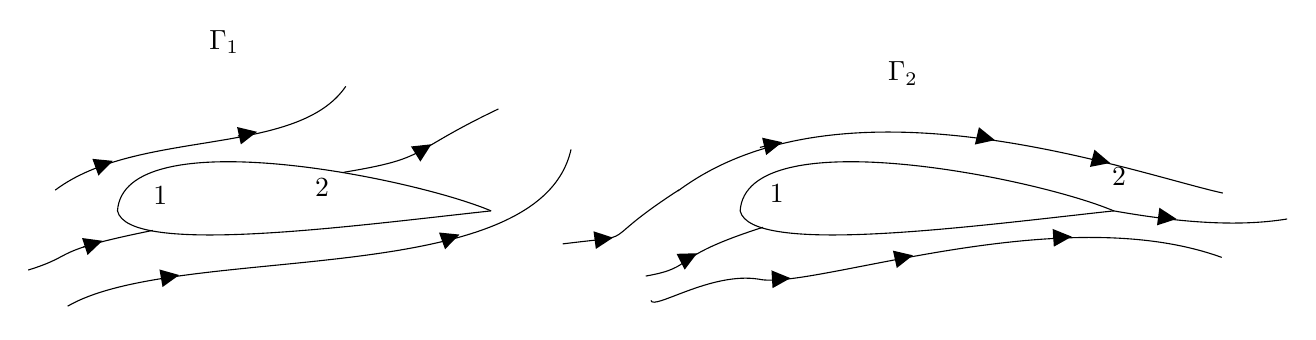
\begin{tikzpicture}[x=0.75pt,y=0.75pt,yscale=-1,xscale=1]
%uncomment if require: \path (0,285); %set diagram left start at 0, and has height of 285

%Curve Lines [id:da757474519234518] 
\draw    (40,120) .. controls (43.01,75.91) and (182.01,103.91) .. (220,120) ;
%Curve Lines [id:da5766387891735065] 
\draw    (40,120) .. controls (45.01,141.91) and (151.51,127.41) .. (220,120) ;
%Curve Lines [id:da7381550438058913] 
\draw    (340,120) .. controls (343.01,75.91) and (482.01,103.91) .. (520,120) ;
%Curve Lines [id:da8883065709307116] 
\draw    (340,120) .. controls (345.01,141.91) and (451.51,127.41) .. (520,120) ;
%Curve Lines [id:da7947732987676788] 
\draw    (10,110) .. controls (50,80) and (126.51,94.41) .. (150,60) ;
%Curve Lines [id:da7784136943432587] 
\draw    (-3,148.5) .. controls (21.51,140.91) and (5.52,139.83) .. (57.01,129.41) ;
%Curve Lines [id:da714986774675068] 
\draw    (16.01,165.91) .. controls (69.51,134.91) and (243.01,159.41) .. (258.51,90.41) ;
%Curve Lines [id:da7768122235559649] 
\draw    (149,101.41) .. controls (191.01,94.41) and (178.51,92.41) .. (223.51,70.91) ;
%Curve Lines [id:da34240417961624026] 
\draw    (294.51,151.41) .. controls (320.01,146.91) and (304.01,142.91) .. (351,127.91) ;
%Curve Lines [id:da0038959201144186384] 
\draw    (519.51,119.91) .. controls (550.51,125.41) and (579.01,127.91) .. (603.51,123.91) ;
%Curve Lines [id:da8381468549415312] 
\draw    (310.01,110.41) .. controls (390.01,50.91) and (529.51,101.91) .. (572.51,111.41) ;
%Curve Lines [id:da4264424078214477] 
\draw    (254.51,135.91) .. controls (294.51,130.91) and (268.01,137.41) .. (310.51,109.91) ;
%Curve Lines [id:da26038258191350194] 
\draw    (349.01,152.91) .. controls (374.01,158.41) and (493.51,113.91) .. (572.01,142.41) ;
%Curve Lines [id:da200973118006885] 
\draw    (297.01,163.16) .. controls (298.01,168.16) and (326.01,149.16) .. (349.01,152.91) ;
%Straight Lines [id:da5173954209160103] 
\draw    (29.51,98.91) -- (34.94,96.94) ;
\draw [shift={(37.76,95.91)}, rotate = 160.02] [fill={rgb, 255:red, 0; green, 0; blue, 0 }  ][line width=0.08]  [draw opacity=0] (8.93,-4.29) -- (0,0) -- (8.93,4.29) -- cycle    ;
%Straight Lines [id:da20555746266271058] 
\draw    (98.01,83.91) -- (104.33,82.55) ;
\draw [shift={(107.26,81.91)}, rotate = 167.8] [fill={rgb, 255:red, 0; green, 0; blue, 0 }  ][line width=0.08]  [draw opacity=0] (8.93,-4.29) -- (0,0) -- (8.93,4.29) -- cycle    ;
%Straight Lines [id:da18452635602009537] 
\draw    (23.51,137.41) -- (29.91,135.34) ;
\draw [shift={(32.76,134.41)}, rotate = 162.03] [fill={rgb, 255:red, 0; green, 0; blue, 0 }  ][line width=0.08]  [draw opacity=0] (8.93,-4.29) -- (0,0) -- (8.93,4.29) -- cycle    ;
%Straight Lines [id:da564713731614449] 
\draw    (61.26,152.41) -- (66.81,151.44) ;
\draw [shift={(69.76,150.91)}, rotate = 169.99] [fill={rgb, 255:red, 0; green, 0; blue, 0 }  ][line width=0.08]  [draw opacity=0] (8.93,-4.29) -- (0,0) -- (8.93,4.29) -- cycle    ;
%Straight Lines [id:da16892046108612524] 
\draw    (196.51,134.41) -- (201.94,132.44) ;
\draw [shift={(204.76,131.41)}, rotate = 160.02] [fill={rgb, 255:red, 0; green, 0; blue, 0 }  ][line width=0.08]  [draw opacity=0] (8.93,-4.29) -- (0,0) -- (8.93,4.29) -- cycle    ;
%Straight Lines [id:da23709222440505573] 
\draw    (184.01,92.41) -- (188.71,89.5) ;
\draw [shift={(191.26,87.91)}, rotate = 148.17] [fill={rgb, 255:red, 0; green, 0; blue, 0 }  ][line width=0.08]  [draw opacity=0] (8.93,-4.29) -- (0,0) -- (8.93,4.29) -- cycle    ;
%Straight Lines [id:da7801353976722618] 
\draw    (271.26,133.91) -- (275.79,133.31) ;
\draw [shift={(278.76,132.91)}, rotate = 172.41] [fill={rgb, 255:red, 0; green, 0; blue, 0 }  ][line width=0.08]  [draw opacity=0] (8.93,-4.29) -- (0,0) -- (8.93,4.29) -- cycle    ;
%Straight Lines [id:da5382263830192704] 
\draw    (349.51,89.41) -- (357.34,87.59) ;
\draw [shift={(360.26,86.91)}, rotate = 166.91] [fill={rgb, 255:red, 0; green, 0; blue, 0 }  ][line width=0.08]  [draw opacity=0] (8.93,-4.29) -- (0,0) -- (8.93,4.29) -- cycle    ;
%Straight Lines [id:da8597748721083103] 
\draw    (454.26,83.91) -- (459.84,85.23) ;
\draw [shift={(462.76,85.91)}, rotate = 193.24] [fill={rgb, 255:red, 0; green, 0; blue, 0 }  ][line width=0.08]  [draw opacity=0] (8.93,-4.29) -- (0,0) -- (8.93,4.29) -- cycle    ;
%Straight Lines [id:da24822087960525052] 
\draw    (510.51,94.91) -- (515.36,96.16) ;
\draw [shift={(518.26,96.91)}, rotate = 194.47] [fill={rgb, 255:red, 0; green, 0; blue, 0 }  ][line width=0.08]  [draw opacity=0] (8.93,-4.29) -- (0,0) -- (8.93,4.29) -- cycle    ;
%Straight Lines [id:da35895933983316564] 
\draw    (311.51,144.41) -- (316.6,141.79) ;
\draw [shift={(319.26,140.41)}, rotate = 152.7] [fill={rgb, 255:red, 0; green, 0; blue, 0 }  ][line width=0.08]  [draw opacity=0] (8.93,-4.29) -- (0,0) -- (8.93,4.29) -- cycle    ;
%Straight Lines [id:da8989308157600859] 
\draw    (356.01,152.91) -- (361.27,152.6) ;
\draw [shift={(364.26,152.41)}, rotate = 176.53] [fill={rgb, 255:red, 0; green, 0; blue, 0 }  ][line width=0.08]  [draw opacity=0] (8.93,-4.29) -- (0,0) -- (8.93,4.29) -- cycle    ;
%Straight Lines [id:da7471632193787989] 
\draw    (416.51,142.91) -- (420.33,142.06) ;
\draw [shift={(423.26,141.41)}, rotate = 167.47] [fill={rgb, 255:red, 0; green, 0; blue, 0 }  ][line width=0.08]  [draw opacity=0] (8.93,-4.29) -- (0,0) -- (8.93,4.29) -- cycle    ;
%Straight Lines [id:da8037532692120464] 
\draw    (492.01,132.91) -- (496.77,132.61) ;
\draw [shift={(499.76,132.41)}, rotate = 176.31] [fill={rgb, 255:red, 0; green, 0; blue, 0 }  ][line width=0.08]  [draw opacity=0] (8.93,-4.29) -- (0,0) -- (8.93,4.29) -- cycle    ;
%Straight Lines [id:da0934187170100993] 
\draw    (542.76,122.91) -- (547.29,123.52) ;
\draw [shift={(550.26,123.91)}, rotate = 187.59] [fill={rgb, 255:red, 0; green, 0; blue, 0 }  ][line width=0.08]  [draw opacity=0] (8.93,-4.29) -- (0,0) -- (8.93,4.29) -- cycle    ;

% Text Node
\draw (83,32) node [anchor=north west][inner sep=0.75pt]    {$\Gamma _{1}$};
% Text Node
\draw (410,47) node [anchor=north west][inner sep=0.75pt]    {$\Gamma _{2}$};
% Text Node
\draw (56,107) node [anchor=north west][inner sep=0.75pt]    {$1$};
% Text Node
\draw (134,103) node [anchor=north west][inner sep=0.75pt]    {$2$};
% Text Node
\draw (353,106) node [anchor=north west][inner sep=0.75pt]    {$1$};
% Text Node
\draw (518,98) node [anchor=north west][inner sep=0.75pt]    {$2$};


\end{tikzpicture}

  \caption{在势流中不同环量值流过翼型在给定攻角。1和2都是驻点}
  \label{fig:stag}
\end{figure}
展示了不同$\Gamma$的流动流过相同翼型在相同攻角的情况。
乍一看,似乎令人进退两难。从实验中,我们知道,给定翼型
在给定攻角的情况下,只会产生一个单值升力。所以,尽管有
无数种势流解,大自然知道如何去选取一种合适的解。显然,
在前述的解法讨论中,并不完全---我们需要一种条件去确定给
定翼型在给定攻角下的$\Gamma$。

为了找到这个条件,让我们先查看一些从静止的初始条件到运动
的绕翼型流动的发展实验情况。流动一开始,流动模式是从绕着
翼型开始发展的。在早期发展的时间,流动是绕着尖后缘点从下
翼面流到上翼面的,和图\ref{fig:stag}中左图相似。然而,更
准确的考虑无粘不可压流动表明,在尖后缘点的速度是无穷大的
。因此,这种流动是不能被大自然长时间容忍的。然而,真实的
流过翼型的流动,在上翼面的驻点会向后缘点移动。最后,在初
始瞬态过程结束后,稳定的流动状态就达到了,即{\color{noteorange}
气流是平滑的从后缘点离开上翼面和下翼面}。这种流动模式就
是图\ref{fig:stag}中的右图,并且表示了在翼型上稳定的流动
类型。

再次强调,给定翼型在给定攻角下建立稳定流动时,大自然会自
动自动产生一个满足要求的特定环量,这个环量使得气流平滑的
离开后缘点。这就是{\bfseries 库塔条件(Kutta condition)}。

为了使库塔条件理论化,我们需要更多的在后缘点的自然流动的
细节。后缘点处可以有一个有限的角度,或者可以是圆弧过渡的。
首先,考虑后缘点处是一个有限角度的情形。记上翼面和下翼面
的速度分别是$V_1$和$V_2$,如图\ref{fig:kutta},
\begin{figure}[!ht]
  \centering
  % ! TEX root = ./Incompressible_Flow_over_Airfoils.tex 

\tikzset{every picture/.style={line width=0.75pt}} %set default line width to 0.75pt        

\begin{tikzpicture}[x=0.75pt,y=0.75pt,yscale=-1,xscale=1]
%uncomment if require: \path (0,285); %set diagram left start at 0, and has height of 285

%Straight Lines [id:da09821137326284046] 
\draw    (110,100) -- (210,130) ;
%Straight Lines [id:da4215300487084799] 
\draw    (210,130) -- (110,160) ;
%Curve Lines [id:da27350478194701067] 
\draw    (110,100) .. controls (86.51,118.41) and (133.51,125.41) .. (110,160) ;
%Straight Lines [id:da5362893989420019] 
\draw    (110,100) -- (136.59,107.85) ;
\draw [shift={(138.51,108.41)}, rotate = 196.44] [color={rgb, 255:red, 0; green, 0; blue, 0 }  ][line width=0.75]    (10.93,-3.29) .. controls (6.95,-1.4) and (3.31,-0.3) .. (0,0) .. controls (3.31,0.3) and (6.95,1.4) .. (10.93,3.29)   ;
%Straight Lines [id:da8226716333160915] 
\draw    (110,99.5) -- (169.6,118.31) ;
\draw [shift={(171.51,118.91)}, rotate = 197.52] [color={rgb, 255:red, 0; green, 0; blue, 0 }  ][line width=0.75]    (10.93,-3.29) .. controls (6.95,-1.4) and (3.31,-0.3) .. (0,0) .. controls (3.31,0.3) and (6.95,1.4) .. (10.93,3.29)   ;
%Straight Lines [id:da8636864097351891] 
\draw    (110,160) -- (192.1,135.49) ;
\draw [shift={(194.01,134.91)}, rotate = 163.37] [color={rgb, 255:red, 0; green, 0; blue, 0 }  ][line width=0.75]    (10.93,-3.29) .. controls (6.95,-1.4) and (3.31,-0.3) .. (0,0) .. controls (3.31,0.3) and (6.95,1.4) .. (10.93,3.29)   ;
%Straight Lines [id:da05016986424572667] 
\draw    (110,160) -- (141.09,150.97) ;
\draw [shift={(143.01,150.41)}, rotate = 163.81] [color={rgb, 255:red, 0; green, 0; blue, 0 }  ][line width=0.75]    (10.93,-3.29) .. controls (6.95,-1.4) and (3.31,-0.3) .. (0,0) .. controls (3.31,0.3) and (6.95,1.4) .. (10.93,3.29)   ;
%Straight Lines [id:da8424011217264318] 
\draw    (110,100) -- (197.09,125.85) ;
\draw [shift={(199.01,126.41)}, rotate = 196.53] [color={rgb, 255:red, 0; green, 0; blue, 0 }  ][line width=0.75]    (10.93,-3.29) .. controls (6.95,-1.4) and (3.31,-0.3) .. (0,0) .. controls (3.31,0.3) and (6.95,1.4) .. (10.93,3.29)   ;
%Straight Lines [id:da6770379071467885] 
\draw    (110,160) -- (168.1,142.49) ;
\draw [shift={(170.01,141.91)}, rotate = 163.23] [color={rgb, 255:red, 0; green, 0; blue, 0 }  ][line width=0.75]    (10.93,-3.29) .. controls (6.95,-1.4) and (3.31,-0.3) .. (0,0) .. controls (3.31,0.3) and (6.95,1.4) .. (10.93,3.29)   ;
%Straight Lines [id:da08219164072740859] 
\draw  [dash pattern={on 4.5pt off 4.5pt}]  (210,130) -- (268.03,139.67) ;
\draw [shift={(270,140)}, rotate = 189.46] [color={rgb, 255:red, 0; green, 0; blue, 0 }  ][line width=0.75]    (10.93,-3.29) .. controls (6.95,-1.4) and (3.31,-0.3) .. (0,0) .. controls (3.31,0.3) and (6.95,1.4) .. (10.93,3.29)   ;
%Straight Lines [id:da8646964142450253] 
\draw  [dash pattern={on 4.5pt off 4.5pt}]  (210,130) -- (268.03,120.33) ;
\draw [shift={(270,120)}, rotate = 170.54] [color={rgb, 255:red, 0; green, 0; blue, 0 }  ][line width=0.75]    (10.93,-3.29) .. controls (6.95,-1.4) and (3.31,-0.3) .. (0,0) .. controls (3.31,0.3) and (6.95,1.4) .. (10.93,3.29)   ;
%Curve Lines [id:da44117033215025336] 
\draw    (380,90) .. controls (420,60) and (460.76,85.41) .. (480,110) ;
%Curve Lines [id:da08129815203793034] 
\draw    (380,120) .. controls (420,90) and (433.26,90.41) .. (480,120) ;
%Curve Lines [id:da34973148212289695] 
\draw    (480,110) .. controls (484.26,114.91) and (484.76,121.41) .. (480,120) ;
%Straight Lines [id:da14103967306792997] 
\draw  [dash pattern={on 4.5pt off 4.5pt}]  (480,110) -- (508.8,148.4) ;
\draw [shift={(510,150)}, rotate = 233.13] [color={rgb, 255:red, 0; green, 0; blue, 0 }  ][line width=0.75]    (10.93,-3.29) .. controls (6.95,-1.4) and (3.31,-0.3) .. (0,0) .. controls (3.31,0.3) and (6.95,1.4) .. (10.93,3.29)   ;
%Straight Lines [id:da8591768857204978] 
\draw  [dash pattern={on 4.5pt off 4.5pt}]  (480,120) -- (503.59,152.79) ;
\draw [shift={(504.76,154.41)}, rotate = 234.26] [color={rgb, 255:red, 0; green, 0; blue, 0 }  ][line width=0.75]    (10.93,-3.29) .. controls (6.95,-1.4) and (3.31,-0.3) .. (0,0) .. controls (3.31,0.3) and (6.95,1.4) .. (10.93,3.29)   ;

% Text Node
\draw (206,100) node [anchor=north west][inner sep=0.75pt]    {$a$};
% Text Node
\draw (226,139) node [anchor=north west][inner sep=0.75pt]    {$V_{1}$};
% Text Node
\draw (229,98) node [anchor=north west][inner sep=0.75pt]    {$V_{2}$};
% Text Node
\draw (496,109) node [anchor=north west][inner sep=0.75pt]    {$V_{1}$};
% Text Node
\draw (459,129) node [anchor=north west][inner sep=0.75pt]    {$V_{2}$};
% Text Node
\draw (479,90) node [anchor=north west][inner sep=0.75pt]    {$a$};
% Text Node
\draw (142,39) node [anchor=north west][inner sep=0.75pt]   [align=left] {有限角度};
% Text Node
\draw (426,39) node [anchor=north west][inner sep=0.75pt]   [align=left] {圆弧};
% Text Node
\draw (110,169) node [anchor=north west][inner sep=0.75pt]   [align=left] {$在点a\text{:}V_1=V_2=0$};
% Text Node
\draw (380,169) node [anchor=north west][inner sep=0.75pt]   [align=left] {$在点a\text{:}V1=V2\neq0$};


\end{tikzpicture}

  \caption{不同后缘点的形状和库塔条件的关系}
  \label{fig:kutta}
\end{figure}
$V_1$是在点$a$平行于上翼面的速度,$V_2$是在点$a$平行于下
翼面的速度。对于一个有限角度的后缘点,如果在点$a$的两个
速度都是有限的,那么我们在同一个点就有两个不同方向的两个速度
,如图\ref{fig:kutta}左图所示。但是,这是在物理上是不可能
的,唯一的办法就是让$V_1$和$V_2$都等于0 。也就是说,对于
有限角度的后缘点,$a$点就是驻点。相反的是,对于圆弧过渡的
后缘点,$V_1$和$V_2$在$a$点方向相同,并且$V_1$和$V_2$都是
有限值。但是,$a$点的压强是一个唯一的值,将伯努利方程
应用于上下翼面接近于$a$点处,得到
\[
  P_a+\frac{1}{2}\rho V_1^2=P_a+\frac{1}{2} \rho V_2^2
\]
或者
\[
  V_1=V_2
\]
因此,对于圆弧过渡的后缘点,我们可以发现,从翼型后缘点离开
上下翼面的速度是有限的,并且大小和方向都是相等的。

我们可以将库塔条件总结表述如下:
\begin{enumerate}
  \item 对于给定翼型在给定攻角的情况下,$\Gamma$的值要使得
    气流平滑地离开后缘点。
  \item 如果后缘角是有限的,那么后缘点就是一个驻点。
  \item 如果后缘角是圆弧过渡的,那么气流在后缘点离开上下翼面的
    速度大小是有限的,并且大小和方向都是一样的。
\end{enumerate}

再次考虑使用面涡模拟翼型的方法,面涡不论是放在翼面还是中弧线上。
沿着面涡的分布,面涡的强度都是变化的,并且记作$\gamma(s)$。库塔
条件使用面涡来表述如下。在后缘点(TE),我们有
\[
  \gamma(\mathrm{TE})=V_1-V_2
\]
然而,对于有限角度的后缘点,$V_1=V_2=0 $;因此,$\gamma(\mathrm{TE})=0 $。
对于圆弧过渡的后缘点,$V_1=V_2\neq 0 $;因此,$\gamma(\mathrm{TE})=0 $。
因此,库塔条件使用面涡表述就是
\begin{empheq}[box=\widefbox]{equation*}
  \gamma(\mathrm{TE})=0 
\end{empheq}

\subsection{没有摩擦能产生升力吗?}
在前面的讨论中,我们强调,浸没在空气中的翼型受到的气动力是
分布在翼型表面上的压强和剪切力的净综合效应。更重要的是,我
们注意到,翼型的升力主要是由于翼面上的压强分布,并且剪应力
对于升力基本上没有影响。这很容易知道是为什么。请看图\ref{fig:stag}
中翼型的形状。回想到压强作用在翼面的法线上,对于这些翼型,
法向的压力基本上是竖直的,也就是升力的方向。
与之相反的是,剪应力作用在翼面的切线方向,对于这些翼型,剪
应力主要是在水平方向,也就是阻力的方向。因此压力是产生升力
的主导者,剪应力对升力的影响可以忽略不记。这就是为什么升力
可以在失速前精准的被无粘理论预测出来,正如本章所讨论的那样。

然而,如果我们生活在一个完美地无粘世界中,翼型就不能产生升力。
事实上,摩擦的存在就是有升力的原因。这听起来很奇怪,甚至与
我们前一段的陈述相互矛盾。为什么会这样?答案就是,在真实生
活中,自然确保气流在后缘点平滑的离开的方法就是自然选择气流
的机制,即粘性边界层一直附着在翼型表面,直到后缘点。自然通
过摩擦来确保达到库塔条件。如果没有粘性边界层(如没有摩擦)
,在自然界中就没有物理机制可以满足库塔条件。

所以我们被代入了最为讽刺的境地,升力是有翼型表面的压强分布
产生的---一种无粘现象,不存在没有摩擦(无粘)的世界中。在
这方面,我们可以说没有摩擦就没有升力。然而,我们以上述讨论
的内容明智地这么说。

\section{开尔文环量定理和启动涡}
库塔条件描述了翼型绕流的环流是一个正值(顺时针为正)确保气
流能平滑的流过后缘点。问题是:这个环量是这么产生的?它是凭
空产生的,还是整个流场的环量都是守恒的呢?

如图\ref{fig:circulation},考虑任意一个无粘、不可压流动。
\begin{figure}[!ht]
  \centering
  % ! TEX root = ./Incompressible_Flow_over_Airfoils.tex

\tikzset{every picture/.style={line width=0.75pt}} %set default line width to 0.75pt        

\begin{tikzpicture}[x=0.75pt,y=0.75pt,yscale=-1,xscale=1]
%uncomment if require: \path (0,360); %set diagram left start at 0, and has height of 360

%Curve Lines [id:da6593875671900111] 
\draw    (110,120) .. controls (239.76,121.41) and (330,70) .. (370,40) ;
%Curve Lines [id:da5152113804444653] 
\draw    (110,180) .. controls (180.76,166.41) and (332.26,111.91) .. (410,120) ;
%Curve Lines [id:da811879248462616] 
\draw    (110,220) .. controls (182.76,209.91) and (376.76,175.41) .. (410,220) ;
%Straight Lines [id:da9503684630542251] 
\draw    (139,120) -- (140.78,119.78) ;
\draw [shift={(143.76,119.41)}, rotate = 172.98] [fill={rgb, 255:red, 0; green, 0; blue, 0 }  ][line width=0.08]  [draw opacity=0] (8.93,-4.29) -- (0,0) -- (8.93,4.29) -- cycle    ;
%Straight Lines [id:da5896891634358687] 
\draw    (190,113.91) -- (193.27,113.65) ;
\draw [shift={(196.26,113.41)}, rotate = 175.43] [fill={rgb, 255:red, 0; green, 0; blue, 0 }  ][line width=0.08]  [draw opacity=0] (8.93,-4.29) -- (0,0) -- (8.93,4.29) -- cycle    ;
%Straight Lines [id:da5521183292347811] 
\draw    (241.5,102.41) -- (244.36,101.67) ;
\draw [shift={(247.26,100.91)}, rotate = 165.41] [fill={rgb, 255:red, 0; green, 0; blue, 0 }  ][line width=0.08]  [draw opacity=0] (8.93,-4.29) -- (0,0) -- (8.93,4.29) -- cycle    ;
%Straight Lines [id:da046097384932481056] 
\draw    (295.76,82.91) -- (298.53,81.66) ;
\draw [shift={(301.26,80.41)}, rotate = 155.56] [fill={rgb, 255:red, 0; green, 0; blue, 0 }  ][line width=0.08]  [draw opacity=0] (8.93,-4.29) -- (0,0) -- (8.93,4.29) -- cycle    ;
%Straight Lines [id:da04541396429043876] 
\draw    (330.26,65.91) -- (332.69,64.46) ;
\draw [shift={(335.26,62.91)}, rotate = 149.04] [fill={rgb, 255:red, 0; green, 0; blue, 0 }  ][line width=0.08]  [draw opacity=0] (8.93,-4.29) -- (0,0) -- (8.93,4.29) -- cycle    ;
%Straight Lines [id:da7876927873324759] 
\draw    (139.76,173.41) -- (140.95,172.97) ;
\draw [shift={(143.76,171.91)}, rotate = 159.44] [fill={rgb, 255:red, 0; green, 0; blue, 0 }  ][line width=0.08]  [draw opacity=0] (8.93,-4.29) -- (0,0) -- (8.93,4.29) -- cycle    ;
%Straight Lines [id:da06331339935669789] 
\draw    (200.76,156.41) -- (203.8,155.91) ;
\draw [shift={(206.76,155.41)}, rotate = 170.54] [fill={rgb, 255:red, 0; green, 0; blue, 0 }  ][line width=0.08]  [draw opacity=0] (8.93,-4.29) -- (0,0) -- (8.93,4.29) -- cycle    ;
%Straight Lines [id:da10300319237850664] 
\draw    (250.26,143.91) -- (252.48,143.03) ;
\draw [shift={(255.26,141.91)}, rotate = 158.2] [fill={rgb, 255:red, 0; green, 0; blue, 0 }  ][line width=0.08]  [draw opacity=0] (8.93,-4.29) -- (0,0) -- (8.93,4.29) -- cycle    ;
%Straight Lines [id:da25013412556469916] 
\draw    (321.76,126.91) ;
\draw [shift={(323.76,126.41)}, rotate = 165.96] [fill={rgb, 255:red, 0; green, 0; blue, 0 }  ][line width=0.08]  [draw opacity=0] (8.93,-4.29) -- (0,0) -- (8.93,4.29) -- cycle    ;
%Straight Lines [id:da6407934074535004] 
\draw    (129.76,217.41) -- (130.78,217.29) ;
\draw [shift={(133.76,216.91)}, rotate = 172.87] [fill={rgb, 255:red, 0; green, 0; blue, 0 }  ][line width=0.08]  [draw opacity=0] (8.93,-4.29) -- (0,0) -- (8.93,4.29) -- cycle    ;
%Straight Lines [id:da4615476728563894] 
\draw    (191.76,208.41) -- (193.28,208.25) ;
\draw [shift={(196.26,207.91)}, rotate = 173.66] [fill={rgb, 255:red, 0; green, 0; blue, 0 }  ][line width=0.08]  [draw opacity=0] (8.93,-4.29) -- (0,0) -- (8.93,4.29) -- cycle    ;
%Straight Lines [id:da9779940169184937] 
\draw    (241.26,202.41) -- (241.79,202.34) ;
\draw [shift={(244.76,201.91)}, rotate = 171.87] [fill={rgb, 255:red, 0; green, 0; blue, 0 }  ][line width=0.08]  [draw opacity=0] (8.93,-4.29) -- (0,0) -- (8.93,4.29) -- cycle    ;
%Straight Lines [id:da9020973429401704] 
\draw    (299.26,197.91) ;
\draw [shift={(301.76,197.41)}, rotate = 168.69] [fill={rgb, 255:red, 0; green, 0; blue, 0 }  ][line width=0.08]  [draw opacity=0] (8.93,-4.29) -- (0,0) -- (8.93,4.29) -- cycle    ;
%Straight Lines [id:da43916377488014824] 
\draw    (357.26,199.41) -- (358.83,199.76) ;
\draw [shift={(361.76,200.41)}, rotate = 192.53] [fill={rgb, 255:red, 0; green, 0; blue, 0 }  ][line width=0.08]  [draw opacity=0] (8.93,-4.29) -- (0,0) -- (8.93,4.29) -- cycle    ;
%Curve Lines [id:da5222840687482979] 
\draw  [dash pattern={on 4.5pt off 4.5pt}]  (140,140) .. controls (180,110) and (216.26,121.5) .. (230,150) ;
%Curve Lines [id:da4165207301071254] 
\draw  [dash pattern={on 4.5pt off 4.5pt}]  (140,140) .. controls (82.76,201.41) and (254.76,227.41) .. (230,150) ;
%Curve Lines [id:da6047764522006289] 
\draw  [dash pattern={on 4.5pt off 4.5pt}]  (290,110) .. controls (330,80) and (397.26,106.41) .. (400,140) ;
%Curve Lines [id:da5317203333510179] 
\draw  [dash pattern={on 4.5pt off 4.5pt}]  (290,110) .. controls (243.76,164.41) and (398.76,213.41) .. (400,140) ;
%Straight Lines [id:da3514021396357123] 
\draw    (100,140) -- (140,140) ;
%Straight Lines [id:da25734728167981236] 
\draw    (400,140) -- (450,130) ;

% Text Node
\draw (79,132.4) node [anchor=north west][inner sep=0.75pt]    {$C_{1}$};
% Text Node
\draw (459,121.4) node [anchor=north west][inner sep=0.75pt]    {$C_{2}$};
% Text Node
\draw (191,42.4) node [anchor=north west][inner sep=0.75pt]    {$\Gamma _{1} =\Gamma _{2}$};
% Text Node
\draw (131,232) node [anchor=north west][inner sep=0.75pt]   [align=left] {流体微团在$t_1$\\时间沿着曲线$C_{1}$};
% Text Node
\draw (307,228) node [anchor=north west][inner sep=0.75pt]   [align=left] {相同的流体微团在\\一段时间后,即$t_2$\\时间,沿着不同的曲线$C_2$中};


\end{tikzpicture}

  \caption{开尔文定律}
  \label{fig:circulation}
\end{figure}
假设所有的彻体力都是0。选择任意一个闭合曲线$C_1$,这条曲线
确定了一定数量的在$t_1$时刻的流体单元。记沿着曲线$C_1$的环
量是$\Gamma_1=-\int _{C_1} \mathbf{V}\cdot \mathrm{d}\mathbf{s}$。
现在,让这些流体单元向下游流动,一段时间后,到达$t_2$时刻。
这些相同的流体单元将来自不同的曲线$C_2$,该曲线确定的环量
是$\Gamma_2=-\int _{C_2} \mathbf{V} \cdot \mathrm{d}\mathbf{s}$。
对于上述描述的状态,我们可以很容易地证明$\Gamma_1=\Gamma_2$。事实
上,我们追踪了一组特定的流体单元,我们可以描述为,由一组
连续的流体单元确定的闭合曲线,随着这些流体单元在全流场中
移动,这条闭合曲线确定的环量是一个常数。关于上述描述的数学
化表述可以简化为
\[
  \frac{\mathrm{D} \Gamma}{\mathrm{D} t}=0
\]
这就是说,有相同的流体单元组成的闭合曲线的环量对时间的变化率
是0。这就是{\bfseries 开尔文环量定理(Kelvin's circulation theoerm)}。
证明过程详见{\color{titleblue}附录\ref{kelvin theroem}}.
开尔文环量定理的一个有趣的结论就是,如果在某个瞬间,一个流动
表面是面涡,那么它将一直保持是面涡。

开尔文环量定理可以帮助解释绕翼型的环量是怎么产生的,如下。
考虑一个翼型在静止的流体中,如图\ref{fig:startvortex}
\begin{figure}[!ht]
  \centering
  % ! TEX root =./Incompressible_Flow_over_Airfoils.tex

\tikzset{every picture/.style={line width=0.75pt}} %set default line width to 0.75pt        

\begin{tikzpicture}[x=0.75pt,y=0.75pt,yscale=-1,xscale=1]
%uncomment if require: \path (0,360); %set diagram left start at 0, and has height of 360

%Shape: Polygon Curved [id:ds1411727865782737] 
\draw   (80,100) .. controls (68.51,32.41) and (201.49,15.59) .. (250,90) .. controls (298.51,164.41) and (269.51,172.41) .. (230,190) .. controls (190.49,207.59) and (161.49,199.59) .. (130,180) .. controls (98.51,160.41) and (91.49,167.59) .. (80,100) -- cycle ;
%Curve Lines [id:da6293293862133582] 
\draw    (120,90) .. controls (148.51,50.41) and (227.51,124.41) .. (240,150) ;
%Curve Lines [id:da44308727702954975] 
\draw    (120,90) .. controls (113.51,105.41) and (198.51,132.41) .. (240,150) ;
%Straight Lines [id:da18147270718988717] 
\draw    (50,60) -- (80,90) ;
%Curve Lines [id:da33190634449649714] 
\draw    (320,80) .. controls (340.76,-1.59) and (565.76,37.91) .. (590,120) ;
%Curve Lines [id:da4273091108123228] 
\draw    (320,80) .. controls (307.76,169.41) and (600.26,160.91) .. (590,120) ;
%Curve Lines [id:da01667939159590026] 
\draw    (350,80) .. controls (354.51,39.91) and (453.51,75.91) .. (460,100) ;
%Curve Lines [id:da44539055148167295] 
\draw    (350,80) .. controls (345.01,94.41) and (406.01,98.41) .. (460,100) ;
%Curve Lines [id:da3052696959417798] 
\draw  [dash pattern={on 4.5pt off 4.5pt}]  (460,100) .. controls (493.26,126.91) and (529.76,136.91) .. (560,130) ;
%Curve Lines [id:da17918828223900296] 
\draw  [dash pattern={on 4.5pt off 4.5pt}]  (540,120) .. controls (543.51,103.41) and (570.01,125.41) .. (560,130) ;
%Curve Lines [id:da6613061331627101] 
\draw    (500,50) .. controls (477.26,67.91) and (511.76,133.91) .. (480,150) ;
%Curve Lines [id:da9665395455277344] 
\draw    (360,60) .. controls (400.44,41.79) and (424.78,47.66) .. (448.55,68.69) ;
\draw [shift={(450,70)}, rotate = 222.34] [color={rgb, 255:red, 0; green, 0; blue, 0 }  ][line width=0.75]    (10.93,-3.29) .. controls (6.95,-1.4) and (3.31,-0.3) .. (0,0) .. controls (3.31,0.3) and (6.95,1.4) .. (10.93,3.29)   ;
%Curve Lines [id:da4858489509606265] 
\draw    (560,110) .. controls (559.03,96.69) and (553.73,85.37) .. (531.39,99.13) ;
\draw [shift={(530,100)}, rotate = 327.31] [color={rgb, 255:red, 0; green, 0; blue, 0 }  ][line width=0.75]    (10.93,-3.29) .. controls (6.95,-1.4) and (3.31,-0.3) .. (0,0) .. controls (3.31,0.3) and (6.95,1.4) .. (10.93,3.29)   ;
%Straight Lines [id:da5834417849984652] 
\draw    (550,120) -- (590,150) ;
%Straight Lines [id:da7932464552251242] 
\draw    (470,150) -- (480,180) ;
%Straight Lines [id:da6750477124024015] 
\draw    (490,150) -- (480,180) ;
%Straight Lines [id:da1468162505445323] 
\draw    (270,90) -- (308,90) ;
\draw [shift={(310,90)}, rotate = 180] [color={rgb, 255:red, 0; green, 0; blue, 0 }  ][line width=0.75]    (10.93,-3.29) .. controls (6.95,-1.4) and (3.31,-0.3) .. (0,0) .. controls (3.31,0.3) and (6.95,1.4) .. (10.93,3.29)   ;
%Straight Lines [id:da11718235105334185] 
\draw    (470,120) -- (490,140) ;
%Straight Lines [id:da4939225263931144] 
\draw    (470,120) -- (451.11,148.34) ;
\draw [shift={(450,150)}, rotate = 303.69] [color={rgb, 255:red, 0; green, 0; blue, 0 }  ][line width=0.75]    (10.93,-3.29) .. controls (6.95,-1.4) and (3.31,-0.3) .. (0,0) .. controls (3.31,0.3) and (6.95,1.4) .. (10.93,3.29)   ;
%Straight Lines [id:da6278616444384559] 
\draw    (490,140) -- (540,160) ;
%Straight Lines [id:da5845827423481111] 
\draw    (540,160) -- (501.94,150.49) ;
\draw [shift={(500,150)}, rotate = 14.04] [color={rgb, 255:red, 0; green, 0; blue, 0 }  ][line width=0.75]    (10.93,-3.29) .. controls (6.95,-1.4) and (3.31,-0.3) .. (0,0) .. controls (3.31,0.3) and (6.95,1.4) .. (10.93,3.29)   ;

% Text Node
\draw (141,92) node [anchor=north west][inner sep=0.75pt]   [align=left] {翼型};
% Text Node
\draw (16,113.4) node [anchor=north west][inner sep=0.75pt]    {$V=0$};
% Text Node
\draw (21,42.4) node [anchor=north west][inner sep=0.75pt]    {$C_{1}$};
% Text Node
\draw (221,12.4) node [anchor=north west][inner sep=0.75pt]    {$\Gamma _{1}$};
% Text Node
\draw (393,2.4) node [anchor=north west][inner sep=0.75pt]    {$\Gamma _{2} =\Gamma _{1} =0$};
% Text Node
\draw (506,22.4) node [anchor=north west][inner sep=0.75pt]    {$\Gamma _{3} =-\Gamma _{4}$};
% Text Node
\draw (478,52.4) node [anchor=north west][inner sep=0.75pt]    {$b$};
% Text Node
\draw (378,72) node [anchor=north west][inner sep=0.75pt]   [align=left] {翼型};
% Text Node
\draw (451,62.4) node [anchor=north west][inner sep=0.75pt]    {$\Gamma _{3}$};
% Text Node
\draw (521,72.4) node [anchor=north west][inner sep=0.75pt]    {$\Gamma _{4}$};
% Text Node
\draw (563,152) node [anchor=north west][inner sep=0.75pt]   [align=left] {启动涡};
% Text Node
\draw (469,181.4) node [anchor=north west][inner sep=0.75pt]    {$C_{2}$};
% Text Node
\draw (271,63.4) node [anchor=north west][inner sep=0.75pt]    {$V\infty $};
% Text Node
\draw (321,43.4) node [anchor=north west][inner sep=0.75pt]    {$a$};
% Text Node
\draw (598,112.4) node [anchor=north west][inner sep=0.75pt]    {$c$};
% Text Node
\draw (471,132.4) node [anchor=north west][inner sep=0.75pt]    {$d$};
% Text Node
\draw (441,111.4) node [anchor=north west][inner sep=0.75pt]    {$C_{3}$};
% Text Node
\draw (531,162.4) node [anchor=north west][inner sep=0.75pt]    {$C_{4}$};
% Text Node
\draw (83,212) node [anchor=north west][inner sep=0.75pt]   [align=left] {翼型周围的流体是静止的};
% Text Node
\draw (361,212.4) node [anchor=north west][inner sep=0.75pt]    {$流体开始流动后的某个瞬间$};


\end{tikzpicture}

  \caption{启动涡和绕翼型环量产生的原因}
  \label{fig:startvortex}
\end{figure}
中左图。因为全流场$\mathbf{V}=0$,所以闭合曲线$C_1$确定的
环量也是0 。现在开始让流体开始运动绕过翼型,气流将倾向于
在后缘周围卷起,如图\ref{fig:startvortex}中右图。这样的话,
后缘点的理论速度将达到无穷大。在真实生活中,这个速度将会是
一个非常大的有限的值。因此,在流动开始的最初时刻,
在后缘点的一个很薄的区域
一个非常大的速度梯度(也就是很大的涡强)就形成了。这个巨大
的涡强被相同的流体单元确定,因此当流体单元向下游流动时,
它被冲到下游。当它向下游运动时,这种薄的很大涡强的单元是
不稳定的,并且它将倾向于向前卷起,形成类似于点涡的图像。
这个涡就叫做{\bfseries 启动涡(starting vortex)},如图
\ref{fig:startvortex}右图所示。当翼型周围的气流达到稳定的
状态后,气流将平滑地流过后缘点(库塔条件),在后缘点
附近的很大的速度梯度也就消失了,在后缘点上也就不在产生涡强了。
然而,启动涡在流动开始流动的过程中已经产生了,并且随着流体
永远地稳定流向下游了。图\ref{fig:startvortex}中右图展示了
稳定流动后的流场,并且在下游某处出现涡流。一开始图\ref{fig:startvortex}
左图组成曲线$C_1$的流体单元流到下游,现在组成了曲线$C_2$,即
闭合曲线$abcda$,如图\ref{fig:startvortex}右图所示。
根据开尔文环量定理,绕曲线$C_2$(包含了翼型和后面的启动涡)
的环量和绕曲线$C_1$的环量是一样的,即都是0。所以
\[
  \Gamma_1=\Gamma_2=0 
\]
现在让我们将曲线$C_2$沿着曲线$bd$分成两个闭合的曲线,即
$C_3(bcdb)$和$C_4(abda)$。曲线$C_4$包围了启动涡,曲线
$C_3$包围了翼型。沿着$C_4$的环量$\Gamma_4$是因为启动涡的存在。
包围翼型的曲线$C_3$的环量是$\Gamma_4$。因为$bc$是曲线$C_3$
和$C_4$的公共边,所以$C_3$和$C_4$的环量之和就等于$C_2$的
环量,即
\[
  \Gamma_3+\Gamma_4=\Gamma_2
\]
然而,我们已经知道$\Gamma_2=0 $,所以
\[
  \Gamma_4=-\Gamma_3
\]
这就是说,绕机翼的环量等于绕启动涡环量的相反数。

这就引出了本节的关键和总结所在。当翼型绕流开始流动,
在尖后缘点处产生的很大的速度梯度产生一个很大的涡强,
这个涡强使得后缘点下游区域的气流卷起来,形成启动涡。
这个启动涡有一个逆时针的环量。因此,一个等大反向的
环量就在翼型上产生了。当这个开始流动过程就继续下去,
后缘点的涡强就不断流入启动涡,使得很大的逆时针环量
变得更大了。相应的,翼型上顺时针的环量也变得更大了,
使得流过后缘点的气流逐渐达到库塔条件,从而减弱了后
缘脱落涡的强度。最后,启动涡达到刚刚满足条件的强度,
使得等大反向的绕翼型的环量导致气流平滑地从后缘流出。
当这种情况发生,从后缘脱落涡的强度就变为了0 ,启动
涡的强度就不在增加了,绕翼型的环量将稳定存在。

\section{经典薄翼理论:对称翼型}
建立翼型的体坐标系,其中$x$沿弦线方向,$z$垂直于
弦线。

对于薄翼型,我们可以用沿中弧线分布的面涡代替这个翼型。
我们的目标是计算出在中弧线成为一条流线,并且满足库塔条件
下的$\gamma(s)$函数。一旦我们找到了一个特定的函数$\gamma(s)$
满足这两个条件,那么我们就可以用积分计算出总的环量,
然后用库塔--茹科夫斯基定理计算相应的升力。

考虑用一个沿中弧线分布的面涡取代翼型的情况。自由来流
的速度是$V_\infty$,翼型的攻角是$\alpha$。如果一个翼型
很薄,那么中弧线非常接近弦线,从很远的地方看,这个面涡
就是沿着弦线分布的。因此,再来一次替换,将沿中弧线的面涡
分布替换成沿弦线的分布,那么$\gamma=\gamma(x)$。我们
依然希望中弧线是流场中的一条流线,并且$\gamma(x)$被计算
出来后依然满足库塔条件,$\gamma(c)=0 $。这就是说,沿弦线
分布的面涡的强度决定了中弧线(不是弦线)是流线。

因为中弧线是流线,所以中弧线上所有点在垂直于中弧线上的
速度分量都是0 。流场中任何一点的速度就是远前方
自由来流的速度和面涡诱导出来的速度的矢量和。记$V_{\infty,n}$
是自由来流在中弧线法向的速度分量,$w'(s)$是由面涡
诱导出来的速度在中弧线法向上的速度分量。因此,因为中弧线
成为了一条流线,所以
\[
  V_{\infty,n}+w'(s)=0 
\]
在中弧线上任意一点都成立,这就是中弧线的边界条件。

对于一个小攻角的薄翼型,有
\[
  V_{\infty,n}=V_\infty(\alpha-\frac{\mathrm{d}z }{\mathrm{d}x})
\]
记$w(x)$是由面涡在弦线上一点诱导出来的速度在法向上的分量,由于
中弧线和弦线非常接近,那么可以做如下近似
\[
  w'(s)\approx w(x)
\]
我们希望计算出在坐标$x$的$w(x)$的值。考虑一个微元涡$\gamma \mathrm{d}\xi$
在沿着弦线距离原点$\xi$的地方。那么在$x$点由$\xi$产生的诱导速度
$\mathrm{d} w $就是
\[
  \mathrm{d} w=- \frac{\gamma(\xi) \mathrm{d} \xi}{2\pi(x-\xi)}
\]
相应的,在$x$点的速度就可以通过积分求解出来,即
\[
  w(x)=-\int _0^c \frac{\gamma (\xi)\mathrm{d}\xi}{2\pi(x-\xi)}
\]
将上面做的两个近似代入到中弧线的边界条件中就有
\[
  V_\infty(\alpha-\frac{\mathrm{d}z }{\mathrm{d}x})-\int _0^c \frac{\gamma(\xi)\mathrm{d}\xi}{2\pi(x-\xi)}=0
\]
或者
\[
  \frac{1}{2\pi}\int _0^c \frac{\gamma(\xi)\mathrm{d}\xi}{x-\xi}=V_\infty(\alpha-\frac{\mathrm{d} z }{\mathrm{d}x})
\]
这就是{\color{noteorange}薄翼理论的基本方程}。这描述了中弧线是流场中的
一条流线。

对于薄翼理论的基本方程,一个给定翼型在给定攻角下,$\alpha$和$\frac{\mathrm{d}z }{\mathrm{d}x}$
都是已知量。实际上,唯一的未知量就是$\gamma(\xi)$。基本方程是一个
积分方程,它的解$\gamma(\xi)$满足中弧线是流线的这个条件。薄翼理论
的核心问题是在满足中弧线是流线的条件下,找到满足库塔条件的解,即
$\gamma(c)=0 $。

如果是一个对称翼,那么
\[
  \frac{1}{2\pi}\int _0^c \frac{\gamma(\xi)\mathrm{d}\xi}{x-\xi}=V_\infty \alpha
\]
可以使用三角换元得到
\[
  \gamma(\theta)=2\alpha V_\infty \frac{1+\cos \theta}{\sin \theta}
\]
于是就有
\[
  \begin{split}
    \frac{1}{2\pi}\int _0^c \frac{\gamma(\theta)\sin  \theta \mathrm{d}\theta}{\cos \theta -\cos \theta_0}
    &=\frac{V_\infty \alpha}{\pi}\int _0^c \frac{(1+\cos \theta)\mathrm{d}\theta}{\cos \theta -\cos \theta_0}\\ 
    &=V_\infty \alpha
  \end{split}
\]
在后缘点处,$\theta=\pi$,那么有
\[
  \gamma(\pi)=2\alpha V_\infty \left.\frac{1+\cos \theta}{\sin \theta}\right| _{\theta=\pi}=
    2\alpha V_\infty \frac{0}{0}
\]
这是一个不确定的极限,使用洛必达法则得到
\[
  \gamma(\pi)=2\alpha V_\infty \frac{-\sin \pi}{\cos \pi}=0 
\]
满足库塔条件。

在这种情况下,现在求解升力系数。绕翼型的总环量是
\[
  \Gamma=\int _0 ^c \gamma(\xi)\mathrm{d}\xi 
\]
使用$\xi=\frac{c}{2 }(1-\cos \theta)$换元得到
\[
  \Gamma=\frac{c}{2}\int _0^\pi \gamma(\theta)\sin \theta \mathrm{d} \theta
\]
将$\gamma(\theta)$代入就可以得到
\[
  \Gamma=\alpha c V_\infty \int_0^\pi (1+\cos \theta)\mathrm{d}\theta =\pi \alpha c V_\infty 
\]
因此单位翼展上的升力就是
\[
  L'=\rho _\infty V_\infty \Gamma =\pi \alpha c V_\infty^2 
\]
因此升力系数就是,其中$S=c(1)$,
\[
  c_l=\frac{L'}{q_\infty S}
\]
得到
\[
  c_l=\frac{L'}{\frac{1}{2}\rho_\infty V_\infty^2 c(1)}=2\pi \alpha
\]
也就是说
\[
  升力曲线的斜率=\frac{\mathrm{d}c_l}{\mathrm{d}\alpha}=2\pi
\]
这是一个重要的结果,它表明了升力系数和攻角是线性相关的。同样,这依然
表明升力曲线的斜率等于$2\pi \,\,\mathrm{rad}^{-1}$。

根据前缘力矩计算公式
\[
  M'_{\mathrm{LE}}=-\int _0^c \xi (\mathrm{d}L)=
  -\rho_\infty V_\infty \int _0^c \xi \gamma(\xi)\mathrm{d}\xi
\]
作积分变换$\xi=\frac{c}{2}(1-\cos \theta)$代入$\gamma(\theta)$
积分得到
\[
  M'_{LE}=-q_\infty c^2 \frac{\pi \alpha}{2}
\]
所以前缘力矩系数就是
\[
  c_{m,le}=\frac{M'_{LE}}{q_\infty S c}
\]
其中,$S=c(1)$,所以前缘力矩系数就是
\[
  c_{m,le}=-\frac{\pi \alpha}{2}
\]
又
\[
  2\pi \alpha =c_l
\]
所以
\[
  c_{m,le}=\frac{c_l}{4}
\]
四分之一弦线处力矩的计算公式是
\[
  c_{m,\frac{c}{4}}=c_{m,le}+\frac{c_l}{4}
\]
所以$\frac{c}{4}$弦线处的力矩即
\[
  c_{m,\frac{c}{4}}=0
\]
这表明了{\color{noteorange}对称翼型的压心在$\frac{c}{4}$弦线处}。由
空气动力学中心的定义,我们得到
{\color{noteorange}对称翼型的气动中心和压心重合,都在$\frac{c}{4}$弦线处}。
\begin{notice}
压心的定义是对压心取矩为0,也就是压心处的气动力矩为0 。

空气动力中心(气动中心)的定义是翼型上存在一点使得对该点
取矩,气动力矩的大小和攻角的变化无关。

注意,当翼型的攻角变大时,压心要往前移,也就是说压心的位置和
攻角大小有关。所以,一般情况下,压心和气动中心不重合。

这里压心和气动中心重合的原因是,首先对$\frac{1}{4 }$弦线
处取力矩为0,所以就是压心。其次,这个力矩恒为0,和攻角
无关,所以就成为了气动中心。
\end{notice}

对本节内容做一个总结如下,对于对称翼型:
\begin{enumerate}
  \item $c_l=2\pi \alpha$ 
  \item 升力曲线的斜率是$2\pi$
  \item 压心和气动中心是重合的,也就是都在$\frac{c}{4}$弦线处
\end{enumerate}
\begin{example}
  考虑一种平盘在攻角$5^\circ$的情况下,计算1)升力系数;2)计算
  前缘力矩系数;3)关于$\frac{c}{4}$弦线处的力矩系数;4)关于
  后缘点的力矩系数;

  \[
    c_l=2 \pi \alpha=\frac{2\pi\times 5}{57.3}=0.5485
  \]
\[
c_{m,le}=- \frac{c_l}{4}=-0.137
\]
\[
  c_{m,\frac{c}{4}}=0
\]
\[
  c_{m,te}=\frac{3}{4}c_l=0.411
\]
\end{example}

对于弧形翼(有弯度的翼型)来说,$\frac{\mathrm{d}z }{\mathrm{d}x}$
不等于0,上述结论就不在适用了。与对称薄翼型一样,中弧线也是流场
中的一条流线,同样满足库塔条件。

同样,基本方程是
\[
  \frac{1}{2\pi}\int _0^c \frac{\gamma(\xi)\mathrm{d}\xi}{x-\xi}=V_\infty (\alpha-\frac{\mathrm{d}z }{\mathrm{d}x})
\]
换元$\xi=\frac{c}{2 }(1-\cos \theta)$,得到
\[
  \frac{1}{2\pi}\int _0^\pi \frac{\gamma(\theta)\sin \theta\mathrm{d}\theta}{\cos \theta -\cos \theta_0}
  =V_\infty \left(\alpha-\frac{\mathrm{d}z }{\mathrm{d}x}\right)
\]
将$\gamma(\theta)$展开成傅里叶正弦级数,即:
\[
  \gamma(\theta)=2V_\infty\left(A_0 \frac{1+\cos \theta}{\sin \theta}+
\sum _{n=1}^\infty A_n \sin n \theta\right)
\]
代入到基本方程中得到
\[
  \frac{1}{\pi}\int _0^\pi \frac{A_0\left(1+\cos \theta\right)\mathrm{d}\theta}{\cos \theta-\cos \theta_0}+
  \frac{1}{\pi}\sum_{n=1}^\infty \int _0^\pi \frac{A_n \sin n \theta \, \mathrm{d}\theta}{\cos \theta-\cos \theta_0}
  =\alpha -\frac{\mathrm{d}z }{\mathrm{d}x}
\]
使用积分结果(见{\color{titleblue}附录\ref{三角函数定积分}}),即:
\[
  \int_0^\pi \frac{\sin n \theta \sin \theta \, \mathrm{d}\theta}{\cos \theta -\cos \theta_0}
  =-\pi \cos n \theta_0
\]
和
\[
  \int _0^\pi \frac{1+\cos \theta}{\cos \theta -\cos \theta_0}\mathrm{d} \theta =\pi
\]
得到
\[
  A_0-\sum _{n=1}^\infty A_n \cos n \theta_0 =\alpha -\frac{\mathrm{d}z }{\mathrm{d} x}
\]
或者
\[
  \frac{\mathrm{d} z }{\mathrm{d}x }=\left(\alpha-A_0\right)+\sum_{n=1}^\infty A_n \cos n \theta_0
\]
上式可以在给定点$x$计算出来,这里$\frac{\mathrm{d}z }{\mathrm{d}x }$和$\theta_0$都是
和弦线上$x$点相关的参数,其中,$x=\frac{c}{2 }(1-\cos \theta_0)$。

回到上面的那个方程,这是将函数$\frac{\mathrm{d}z }{\mathrm{d}x}$用
傅里叶余弦级数展开的。那么函数$f(\theta)$可以用级数来表示
\[
  f(\theta)=B_0+\sum_{n=1}^\infty \cos n \theta
\]
其中,$0\leq \theta \geq \pi$。系数可以用如下的方法计算出来:
\[
  B_0=\frac{1}{\pi} \int _0^\pi f(\theta) \, \mathrm{d} \theta
\]
和
\[
  B_n=\frac{2}{\pi}\int _0 ^\pi f(\theta)\cos n \theta\, \mathrm{d} \theta
\]
$\frac{\mathrm{d} z }{\mathrm{d} x}$和$f(\theta)$是一样的,所以
\[
  \alpha-A_0=\frac{1}{\pi}\int _0^\pi \frac{\mathrm{d}z }{\mathrm{d}x }\, \mathrm{d} \theta_0
\]
和
\[
  A_n=\frac{2}{\pi}\int _0 ^\pi \frac{\mathrm{d} z }{\mathrm{d}x}\cos n \theta_0\,
  \mathrm{d} \theta_0
\]
请记住,$\frac{\mathrm{d}z }{\mathrm{d}x}$是关于$\theta_0$的函数。
从上面的方程可以看出,$A_0$与飞行迎角和中弧线的形状有关系,但是$A_n$
只和中弧线的形状有关。

在上面的讨论中,我们考虑了
气流流过一个有弯度的翼型在给定的形状$\frac{\mathrm{d}z }{\mathrm{d}x}$
和给定的攻角。为了使得中弧线成为流线,我们需要计算出沿弦线的面涡强度分布。
同样,也要满足库塔条件。$A_0$和$A_n$的实际数值可以在给定攻角下通过简单
的积分计算得到。当$\mathrm{d}z / \mathrm{d}x =0$的时候,那就是一个对称
翼型,是上述积分计算公式的一种特殊情况。

下面我们计算对于一个有弯度的翼型的空气动力系数。从前缘点到后缘点的
总环量可以通过下面的积分得到
\[
  \Gamma=\int _0^c \gamma(\xi)\,\mathrm{d}\xi =
  \int _0^\pi \gamma(\theta)\, \mathrm{d}\theta
\]
将我们得到的$\gamma(\theta)$代入到上式得到
\[
  \Gamma=c V_\infty \left[A_0\int _0^\pi \left(1+\cos \theta\right)\,\mathrm{d}\theta
+\sum _{n=1}^\infty A_n\int _0^\pi \sin n \theta \sin \theta \,\mathrm{d}\theta\right]
\]
其中
\[
  \int _0^\pi (1+\cos \theta)\, \mathrm{d} \theta=\pi
\]
\[
  \int _0^\pi \sin n \theta \sin \theta \,\mathrm{d}\theta =
  \begin{cases}
    \frac{\pi}{2 }&,n=1 \\ 
    0 &,n\neq 1
  \end{cases}
\]
因此,总环量就是
\[
  \Gamma=c V_\infty \left(\pi A_0 +\frac{\pi}{2 }A_1\right)
\]
根据库塔--茹科夫斯基定理得到单位翼展上的升力
\[
  L'=\rho_\infty V_\infty \Gamma=
  \rho_\infty V_\infty^2 c\left(\pi A_0+\frac{\pi}{2 }A_1\right)
\]
那么升力系数就是
\[
  c_l=\frac{L'}{\frac{1}{2 }\rho_\infty V_\infty ^2 c(1)}=\pi(2A_0+A_1)
\]
代入$A_0$和$A_1$的计算公式得到
\[
  c_l=2\pi \left[\alpha+\frac{1}{\pi}\int _0^\pi \frac{\mathrm{d}z }{\mathrm{d}x}(\cos \theta_0-1)
  \, \mathrm{d}\theta_0\right]
\]
也就是
\begin{empheq}[box=\widefbox]{equation*}
  升力线斜率=\frac{\mathrm{d}c_l }{\mathrm{d}\alpha}=2\pi
\end{empheq}
记住这是一个重要结果,对于对称翼型和有弯度的翼型升力线斜率都是$2\pi$。
事实上,这个从薄翼理论得到的结果对于所有翼型都适用,也就是所有
翼型的升力线斜率都是$2\pi$。请注意,对称翼型的升力系数$c_l$和有
弯度的翼型的升力系数是有区别的。回忆零升攻角$\alpha_{L=0}$的概念,
它一般是一个负值,升力线的方程可以写成
\[
  c_l=\frac{\mathrm{d}c_l}{\mathrm{d}\alpha}(\alpha-\alpha_{L=0})
\]
也即是 
\[
  c_l=2\pi(\alpha-\alpha_{L=0})
\]
比较我们推导的升力线方程,可以得到
\[
  \alpha_{L=0}=-\frac{1}{\pi}\int _0^\pi \frac{\mathrm{d}z }{\mathrm{d}\alpha}
  (\cos \theta_0-1)\,\mathrm{d}\theta_0
\]
这个方程提供了一种方法去预测零升攻角的大小。对于对称翼型的零升攻角就是0 。
相应的,对于弯度比较大的翼型,它的零升攻角的值就要大一些。

根据前缘力矩的定义
\[
  M'_{\mathrm{LE}}=-\int _0^c \xi (\mathrm{d}L)=
  -\rho_\infty V_\infty \int _0^c \xi \gamma(\xi)\mathrm{d}\xi
\]
换元,并将$\gamma(\theta)$代入,计算得到
\[
  c_{m,le}=-\frac{\pi}{2 }\left(A_0+A_1-\frac{A_2}{2}\right)
\]
将升力系数代入得到
\[
  c_{m,le}=-\left[\frac{c_l}{4}+\frac{\pi}{4}(A_1-A_2)\right]
\]
当$\mathrm{d}z /\mathrm{d}x=0$,即$A_1=A_2=0 $,代入到上式
就得到了对称翼型的前缘力矩。

$\frac{c}{4}$处的力矩可以通过
\[
  c_{m,\frac{c}{4}}=c_{m,le}+\frac{c_l}{4}
\]
计算得到
所以
\[
  c_{m,\frac{c}{4}}=-\frac{\pi}{4}\left(A_1-A_2\right)
\]
不像对称翼型那样,有弯度的翼型$\frac{c}{4}$处的力矩不等于0 。
上式表明,四分之一弦线处的力矩是有限的。然而$A_1$和$A_2$是
只和翼型的弯度大小有关的,而与攻角大小无关。所以
四分之一弦线处是有弯度翼型的理论的气动中心。

压心的位置可以通过下面的公式计算得到
\[
  x_{cp}=-\frac{M'_{LE}}{L'}=-\frac{c_{m,le}c}{L'}
\]
也就是
\[
  x_{cp}=\frac{c}{4}\left[1+\frac{\pi}{c_l}\left(A_1-A_2\right)\right]
\]
这表明有弯度翼型的压心位置是随着升力系数的大小变化而变化的。
因此,攻角变化,压心也随着变化。事实上,当升力趋向于0,
$x_{cp}$就移动到无穷远处了;这就是说,它离开了翼型。因为
这样,压心并不是一个很方便的点来描述翼型上的力系。反而,
气动中心就十分方便来描述翼型上的力系和力矩系。

\begin{example}
  给定翼型NACA 23012 。这个翼型的中弧线方程是
  \[
    \frac{z}{c}=2.6595\left[\left(\frac{x}{c}\right)^3 -0.6075
    \left(\frac{x}{c}\right)^2 +0.1147\left(\frac{x}{c}\right) 
  \right] \qquad 0\leq \frac{x}{c} \geq 0.2025 
  \]
  和
  \[
    \frac{z}{c}=0.02208\left(1-\frac{x}{c}\right) \qquad 0.2025 \leq \frac{x}{c} \geq 1.0 
  \]

计算a)零升攻角;b)$\alpha=4^\circ$时的升力系数;c)四分之一
弦线处的气动力矩系数;d)$\alpha=4^\circ$时的压心的位置,用$x_{cp} / c $表示。

首先,我们需要计算出$\frac{\mathrm{d}z }{\mathrm{d} x}$。对于给定的中弧线,有
\[
  \frac{\mathrm{d}z }{\mathrm{d}x}=2.6595
  \left[3\left(\frac{x}{c}\right)-1.215\left(\frac{x}{c}\right)+0.1147\right]
  \qquad 0 \leq \frac{x}{c} \geq 0.2025
\]
和
\[
  \frac{\mathrm{d}z }{\mathrm{d}x}=0.02208 \qquad 0.2025 \leq \frac{x}{c} \geq 1.0
\]
将坐标$x$变换到$\theta$,即$x=\frac{c}{2}(1-\cos \theta)$,我们有
\[
  \begin{split}
    \frac{\mathrm{d}z }{\mathrm{d}x}&=2.6595
  \left[\frac{3}{4}(1-2\cos \theta +\cos ^2 \theta)-0.6075(1-\cos \theta)+0.1147\right] \\ 
                                    &=
                                    0.6840-2.3736 \cos \theta +1.995 \cos ^2 \theta
                                    \qquad  0 \leq \theta \geq 0.9335 \,\,\mathrm{rad}
  \end{split}
\]
和
\[
  \frac{\mathrm{d}z }{\mathrm{d} x}=-0.02208 \qquad 0.9335 \leq \theta \geq \pi
\]
(a)
\[
  \alpha_{L=0}=\int _0^\pi \frac{\mathrm{d}z }{\mathrm{d}x}(\cos \theta-1)\,\mathrm{d}\theta=
  -0.0191\,\, \mathrm{rad}
\]
(b)
$\alpha=4^\circ=0.0698 \,\,\mathrm{rad}$,
\[
  c_l=2\pi (\alpha-\alpha_{L=0})=2\pi(0.0698+0.0191)=0.559
\]
(c)
我们需要先计算出$A_1$和$A_2$的值。
\[
  A_1=\frac{2}{\pi}\int _0^\pi \frac{\mathrm{d}z }{\mathrm{d}x }\cos \theta\,\mathrm{d} \theta
  =0.0954
\]
\[
  A_2=\frac{2}{\pi}\int _0^\pi \frac{\mathrm{d}z }{\mathrm{d}x} \cos 2 \theta\, \mathrm{d} \theta
  =0.0792
\]
于是
\[
  c_{m,\frac{c}{4}}=\frac{\pi}{4}(A_2-A_1)=\frac{\pi}{4}(0.0792-0.0954)=-0.0127
\]
(d)
由
\[
  x_{cp}=\frac{c}{4}\left[1+\frac{\pi}{c_l}\left(A_1-A_2\right)\right]
\]
于是
\[ 
  \begin{split}
    \frac{x_{cp}}{c}&=\frac{1}{4}\left[1+\frac{\pi}{c_l}\left(A_1-A_2\right)\right]\\
                    &=\frac{1}{4}\left[1+\frac{\pi}{0.559}(0.0954-0.0792)\right]=0.273
  \end{split}
\]
\end{example}

至此,本节的任务已经全部完成了。本节内容我们计算了薄翼型的升力系数,力矩系数
和前缘力矩等,还证明了升力线的斜率是$2\pi$。



% !TEX root = ../mechanics.tex
\section{关于气动中心的额外讨论}
在前面薄翼理论中,我们证明了气动中心不仅是
真实存在的,而且位置在翼型的四分之一的弦线
处。因此,我们可以增加一种新的方法来描述翼
型上的气动力和气动力矩,也就是气动力和气动
力矩通过气动中心。

对于大部分常规的翼型,不是很精确地说,气动
中心都是比较靠近四分之一弦线这个位置。只要
给出任意一个翼型的气动力系数曲线和气动力矩
系数曲线,我们都可以按照下面的方法计算出气
动中心的位置。考虑对四分之一弦线出取力矩和
升力的升力力矩系。将气动中心到前缘点的距离
记为
$c \overline{x}_{ac}$,
将气动中心记作ac,于是我们有
\[
	M'_{ac}=L'\left(c \overline{x}_{ac}-\frac{c}{4}\right)+M'_{\frac{c}{4}}
\]
上式两边同时除以
$q_\infty Sc$
我们得到
\[
	c_{m,ac}=c_l(\overline{x}_{ac}-\frac{1}{4})+c_{m,\frac{c}{4}}
\]
对上式两边同时对攻角$\alpha$取微分,我们有
\[
	\frac{\mathrm{d}c_{m,ax}}{\mathrm{d}\alpha}
	=\frac{\mathrm{d}c_l}{\mathrm{d}\alpha}(\overline{x}_{ac}-\frac{1}{4})
	+\frac{\mathrm{d}c_{m,\frac{c}{4}}}{\mathrm{d}\alpha}
\]
根据气动中心定义,有
\[
	\frac{\mathrm{d}c_{m,ac}}{\mathrm{d}\alpha}=0
\]
所以
\[
	0=\frac{\mathrm{d}c_l}{\mathrm{d}\alpha}(\overline{x}_{ac}-\frac{1}{4})
	+\frac{\mathrm{d}c_{m,\frac{c}{4}}}{\mathrm{d}\alpha}
\]
对于一个尚未达到失速的翼型,升力系数曲线和力矩系数曲线的
斜率都是一个常数,所以
\[
	\frac{\mathrm{d}c_l}{\mathrm{d}\alpha}=a_0 \qquad
	\frac{\mathrm{d}c_{m,\frac{c}{4}}}{\mathrm{d}\alpha}=m_0
\]
就得到了
\[
	0=a_0(\overline{x}_{ac}-\frac{1}{4})+m_0
\]
或者
\[
	\overline{x}_{ac}=-\frac{m_0}{a_0}+\frac{1}{4}
\]
这个方程证明了,对于一个有着线性的升力线和力矩线
的翼型来说,气动中心的位置就是固定的。当然,这还
给出了一个计算气动中心位置的方法。

\section{粘性流动:翼型阻力}
我们知道翼型的升力主要是翼面上的压强分布产生的;
翼面上的剪切力的分布在沿升力方向上的积分通常是
微不足道的。因此,升力可以通过无粘不可压流动结合
后缘点的库塔条件被精确地计算出来。当需要去预测
阻力的时候,这个方法得到的结果就是0 ,这个结果
和常见的场景是截然相反的,这就是达朗贝尔谬论。

直到粘性这个概念引入流动,这个悖论才被解决。
事实上,粘性完全是翼型产生阻力的原因。它通过
两种机制产生作用:
\begin{enumerate}
	\item 表面摩擦阻力,即主要由翼型表面上的剪切力分布产生的;
	\item 压差阻力,主要是由流动分离产生的,也叫做型阻;
\end{enumerate}
剪切力产生阻力是显而易见的,流动分离产生阻力是一个微妙
的现象,我们将在后面讨论。
\subsection{估计表面摩擦阻力:层流}
作为一种近似,我们假设一个翼型上的表面
摩擦阻力和一块平板上的表面摩擦阻力是一
样的,如图\ref{fig:plate}。
\begin{figure}[!ht]
	\centering
	% ! TEX root = ./Incompressible_Flow_Airfoil_2.tex

\tikzset{every picture/.style={line width=0.75pt}} %set default line width to 0.75pt        

\begin{tikzpicture}[x=0.75pt,y=0.75pt,yscale=-1,xscale=1]
%uncomment if require: \path (0,300); %set diagram left start at 0, and has height of 300

%Shape: Rectangle [id:dp8246665344533497] 
\draw  [fill={rgb, 255:red, 74; green, 144; blue, 226 }  ,fill opacity=1 ] (90.39,122.31) -- (540,122.31) -- (540,140) -- (90.39,140) -- cycle ;
%Curve Lines [id:da111522274445083] 
\draw  [dash pattern={on 4.5pt off 4.5pt}]  (90.39,122.31) .. controls (97.1,85.96) and (417.76,18.63) .. (530,20) ;
%Straight Lines [id:da9873373468406699] 
\draw [line width=3]    (280,130) -- (384,130) ;
\draw [shift={(390,130)}, rotate = 180] [fill={rgb, 255:red, 0; green, 0; blue, 0 }  ][line width=0.08]  [draw opacity=0] (16.97,-8.15) -- (0,0) -- (16.97,8.15) -- cycle    ;
%Straight Lines [id:da3618853648976492] 
\draw    (10,130) -- (78,130) ;
\draw [shift={(80,130)}, rotate = 180] [color={rgb, 255:red, 0; green, 0; blue, 0 }  ][line width=0.75]    (10.93,-3.29) .. controls (6.95,-1.4) and (3.31,-0.3) .. (0,0) .. controls (3.31,0.3) and (6.95,1.4) .. (10.93,3.29)   ;
%Straight Lines [id:da2969004979431211] 
\draw    (90,150) -- (90,180) ;
%Straight Lines [id:da7604315764856493] 
\draw    (540,150) -- (540,180) ;
%Straight Lines [id:da1544757975714104] 
\draw    (290,170) -- (538,170) ;
\draw [shift={(540,170)}, rotate = 180] [color={rgb, 255:red, 0; green, 0; blue, 0 }  ][line width=0.75]    (10.93,-3.29) .. controls (6.95,-1.4) and (3.31,-0.3) .. (0,0) .. controls (3.31,0.3) and (6.95,1.4) .. (10.93,3.29)   ;
%Straight Lines [id:da8380825014920565] 
\draw    (290,170) -- (92,170) ;
\draw [shift={(90,170)}, rotate = 360] [color={rgb, 255:red, 0; green, 0; blue, 0 }  ][line width=0.75]    (10.93,-3.29) .. controls (6.95,-1.4) and (3.31,-0.3) .. (0,0) .. controls (3.31,0.3) and (6.95,1.4) .. (10.93,3.29)   ;
%Straight Lines [id:da2973110443382847] 
\draw    (90,160) -- (198,160) ;
\draw [shift={(200,160)}, rotate = 180] [color={rgb, 255:red, 0; green, 0; blue, 0 }  ][line width=0.75]    (10.93,-3.29) .. controls (6.95,-1.4) and (3.31,-0.3) .. (0,0) .. controls (3.31,0.3) and (6.95,1.4) .. (10.93,3.29)   ;
%Straight Lines [id:da8687841920204464] 
\draw    (500,70) -- (500,119.96) ;
\draw [shift={(500,121.96)}, rotate = 270] [color={rgb, 255:red, 0; green, 0; blue, 0 }  ][line width=0.75]    (10.93,-3.29) .. controls (6.95,-1.4) and (3.31,-0.3) .. (0,0) .. controls (3.31,0.3) and (6.95,1.4) .. (10.93,3.29)   ;
%Straight Lines [id:da08951308827383575] 
\draw    (500,70) -- (500,22) ;
\draw [shift={(500,20)}, rotate = 90] [color={rgb, 255:red, 0; green, 0; blue, 0 }  ][line width=0.75]    (10.93,-3.29) .. controls (6.95,-1.4) and (3.31,-0.3) .. (0,0) .. controls (3.31,0.3) and (6.95,1.4) .. (10.93,3.29)   ;

% Text Node
\draw (22,99) node [anchor=north west][inner sep=0.75pt]    {$V_{\infty }$};
% Text Node
\draw (309,99) node [anchor=north west][inner sep=0.75pt]   [align=left] {阻力};
% Text Node
\draw (306,150) node [anchor=north west][inner sep=0.75pt]    {$c$};
% Text Node
\draw (136,140) node [anchor=north west][inner sep=0.75pt]    {$x$};
% Text Node
\draw (506,60) node [anchor=north west][inner sep=0.75pt]    {$\delta $};


\end{tikzpicture}

	\caption{平板上的总摩擦阻力}
	\label{fig:plate}
\end{figure}
显然,这种近似对于更薄的翼型和更小的攻角是更加
准确的。

我们首先来计算层流流过翼型(或者是薄平板)的情况。
对于层流边界层是有精确的解析解的。

对于一个不可压层流在零攻角的情况下流过薄平板,边界层
厚度的计算公式如下
\[
	\delta=\frac{5.0 x}{\sqrt{Re_x}}
\]
其中,$Re_x$是距离前缘$x$处的雷诺数,也就是
\[
	Re_x=\frac{\rho_e V_\infty x }{\mu_\infty}
\]
也就是$\delta \propto \sqrt{x } $,也就是
边界层的厚度随着到前缘点的距离抛物线地增长。

当地的剪切应力沿着平板的上下表面积分就得到了最终
的摩擦阻力,$D_f$。首先,不管怎样,我们先考虑
平板的一个表面,不论是上表面还是下表面。剪切
力在上下表面的分布是一样的。让我们选择上表面。
在整个上表面对剪切力积分得到最终的上表面的
摩擦阻力,$D_{f,top}$。显然这个阻力大小和下表面
的阻力大小,$D_{f,bot tom}$,是一样大的。
因此,总的摩擦阻力就是
\[
	D_f=2D_{f,top}=2D_{f,bot tom}
\]
定义一个表面的阻力系数是
\[
	C_f=\frac{D_{f,top}}{q_\infty S }=\frac{D_{f,bot tom}}{q_\infty S }
\]
表面摩擦阻力系数是雷诺数的函数,即
\[
	C_f=\frac{1.328}{\sqrt{Re_c}}
\]
其中$Re_c$通过如下公式计算
\[
	Re_c=\frac{\rho_\infty V_\infty c }{\mu_\infty}
\]

对于一个非常大的雷诺数的流动,翼型边界层内的流动是
湍流。我们的层流计算就不足以近似估计边界层厚度和翼
型的阻力系数了。让我们采取下一步。

\subsection{估计表面摩擦阻力:湍流}
和层流的情况相反,对于湍流边界层是没有精确的解析解的。
对于任意湍流的分析需要大量的数据。湍流的分析都是近似
的。

流过平板的湍流边界层的分析是不例外的。我们直接给出这个
经验公式
\[
	\delta = \frac{0.37 x }{Re_x ^{\frac{1}{5 }}}
\]
阻力系数计算公式如下
\[
	C_f=\frac{0.074}{Re_c^{\frac{1}{5 }}}
\]
这里再次强调,上面两个公式都是近似结果,并且
它们只代表了对于平板湍流边界层的一组大量的
不同湍流分析的实验数据。然而,这两个公式给了
我们估计湍流边界层厚度和表面摩擦阻力系数的一个
方法。

值得注意的是,这种估计湍流表面摩擦阻力的计算公式
过高估计了表面摩擦阻力系数。实际上,在距离前缘点
的一段距离内,边界层总是起始于层流边界层,在前缘点
后的某个点之后开始向湍流边界层转捩。因此表面摩擦阻力
是层流边界层和湍流边界层的组合。接下来,让我们开始
检查这种情况。

\subsection{转捩}
前面的讨论中,我们分别假设了平板的边界层分别
全是层流和全是湍流。然后在前缘下游的某个点开
始,层流边界层开始变得不稳定,变成湍流边界层。
层流边界层向湍流边界层发展的区域叫做转捩区域。
在这个区域之后,边界层全部都是湍流边界层。记
转捩点的位置是$x_cr$,这是一个临界位置,这个
位置的雷诺数叫做临界雷诺数,$Re_{cr}$,计算
公式如下
\[
	Re_{cr}=\frac{\rho_\infty V_\infty x_cr}{\mu_\infty}
\]
如果给出临界雷诺数,那么临界位置也就能计算出
来了。大量的实验表明,临界雷诺数大约是$5\times 10^5 $。

总的来说,只要你知道了临界雷诺数,就能计算出
转捩点。然而,精确的临界雷诺数必须来自实验,
惯性飞行或者是一些半实验理论。

对于边界层有转变的边界层阻力系数的计算,我们
可以先假设整个边界层都是湍流边界层,这样计算
的结果肯定是偏大的,然后分别计算出转捩点之前
的层流边界层的阻力系数和湍流边界层的阻力系数。
最后,将全湍流边界层的阻力系数减去转捩点之前
的湍流边界层的阻力系数,再加上转捩点之前的层
流边界层的阻力系数,这样就得到了边界层有转捩
的阻力系数。

\subsection{流动分离}
翼型上的压差阻力是由流动分离造成的。对于气流
全部附在翼型表面的流动来说,翼型后面的压强产
生的向前的力会被翼型前面压强产生的向后的力抵
消掉。这就导致了零压差阻力。然而,如果流过翼
型后表面的气流部分分离,这就会导致翼型后面的
压强产生的向前的力比流体全部附在翼型上的情况
小,即不能和翼型前面压强产生的向后的力全部抵
消掉,从而产生了一个净压差阻力---这个压差阻力
是由于流动分离产生的。

那么什么情况有助于流动分离呢?为了回答这个问
题,首先考虑气体在零攻角的情况下流过一个翼型。
流线平滑地经过翼型的表面---没有任何的流动分离。
计算流体力学的结果表明,这种情况下,翼型的前
缘点是驻点,压强系数
$C_P=1.0$
,然后上翼面的气流快速地膨胀,压强急剧减小,
在上翼面前缘点下游的某个位置达到最小值。然后
随着气流往下游流去,压强逐渐增加,在后缘点的
压强比自由来流的压强稍大。这个压强增大的区域
叫做{\bfseries 逆压梯度区(adverse pressuer gradient)}。
通过定义,逆压梯度区的压强是随着流动方向增强
的。这个区域的$\frac{\mathrm{d}P }{\mathrm{d}x}$
是正值。逆压梯度区是变化不大的,也就是
$\frac{\mathrm{d}P }{\mathrm{d}x }$是比较小的。
对于所有的实际情况,气流依然保持附在翼型的表面
上,除了后缘点附近的区域。

现在,我们考虑一个相同的翼型在攻角很大的情况
下。假设这是一个纯粹的没有流动分离的无粘流动
---一种纯粹的理想情况。在这种理想情况下,数值
解表明,在前缘点下游的某个点,压强会急剧地下
降到$C_P=-9$,然后在下游快速地上升,在后缘点
恢复到比$P_\infty$稍大的一个值。在这个恢复的
过程中,压强是急剧变大的,这和我们前面讨论的
零攻角的情况是相反的。这个逆压梯度区的变化是
很大的,所以,$\frac{\mathrm{d}P }{\mathrm{d}x }$
是非常大的。在这种情况下,真实的粘性流将要从
翼型的表面分离。这种情况下,压强没有急剧地下
降到一个最小值,后缘点的压强也没有恢复到$P_\infty$。

请看这两种情况下翼型上的压强分布图,如图
\ref{fig:sepratedflow}。
\begin{figure}[!ht]
  \centering
  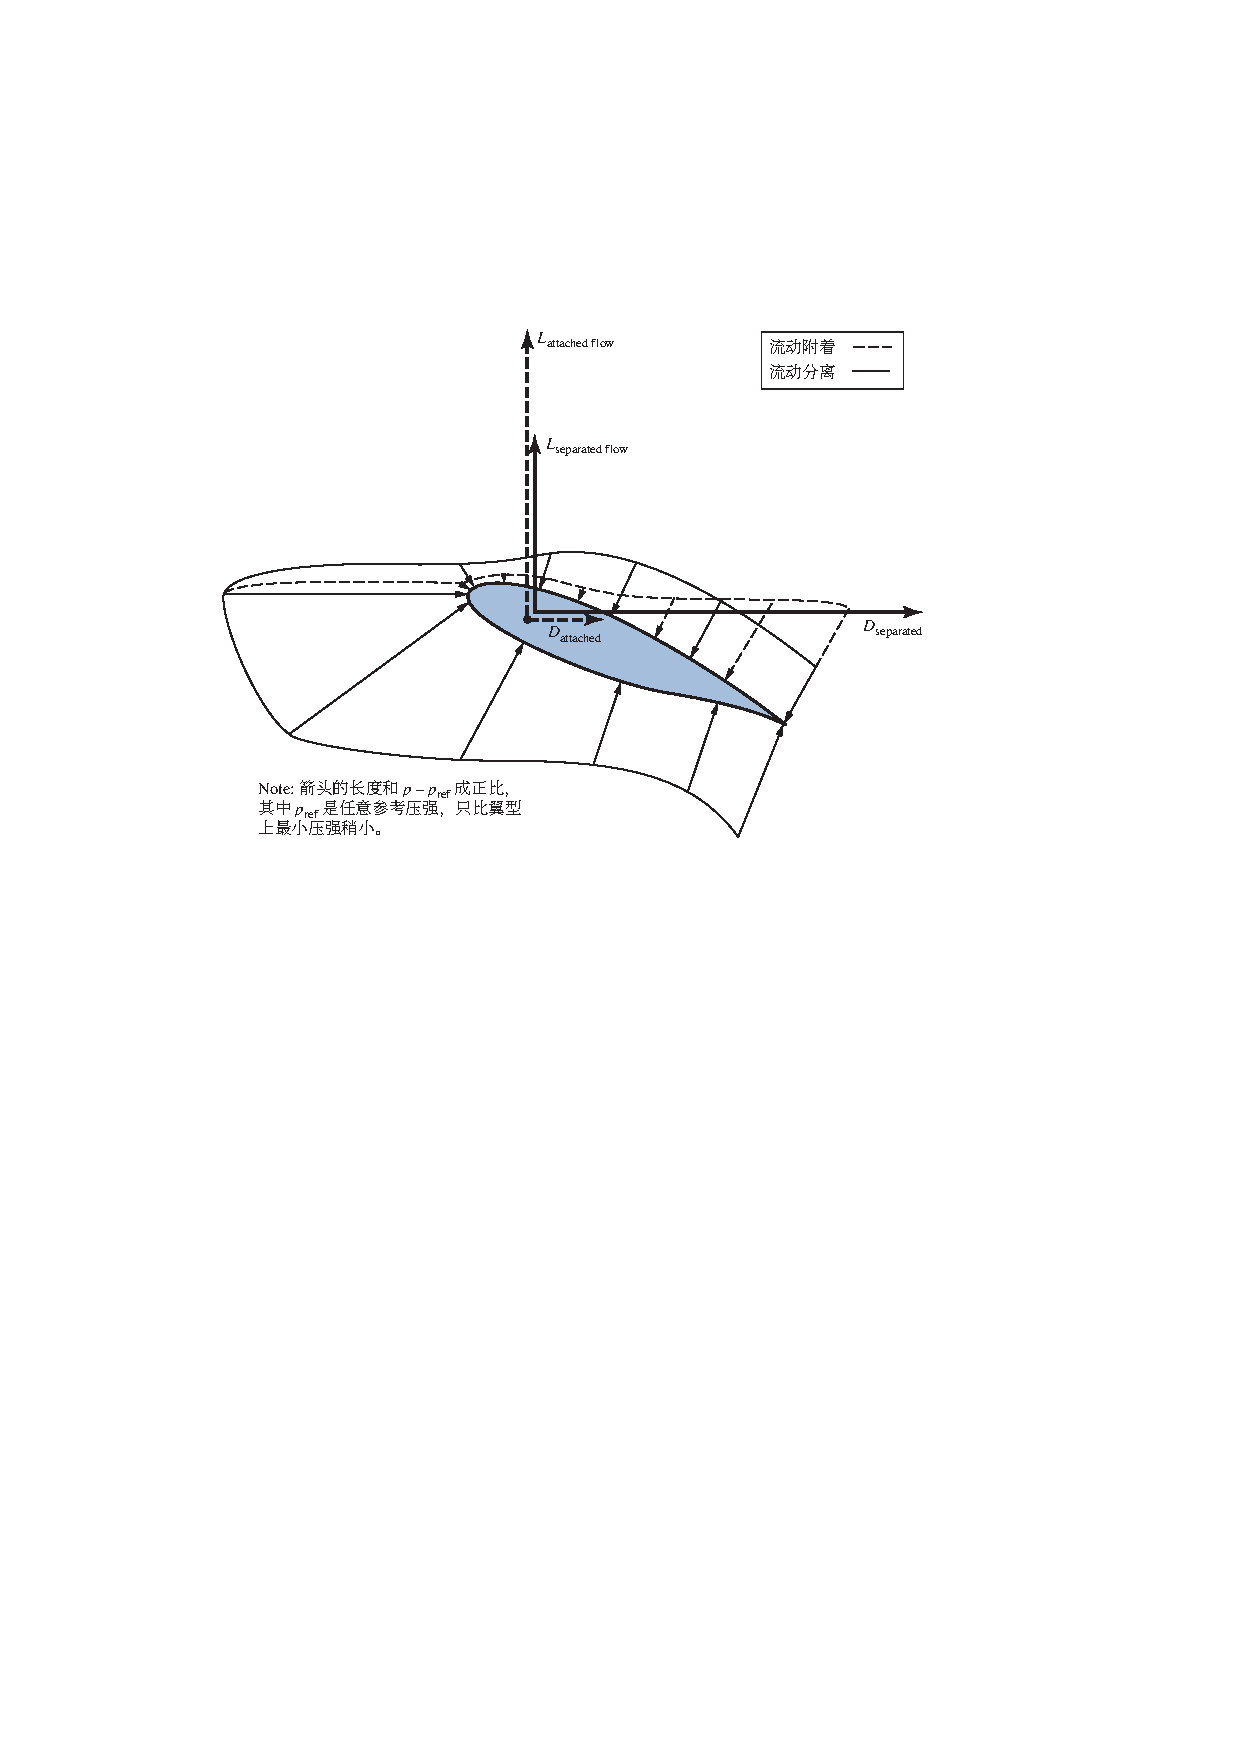
\includegraphics[height=10cm]{./aerodynamics/seprated_flow.pdf}
  \caption{流动分离与流动附着时的对比}
  \label{fig:sepratedflow}
\end{figure}
图中,在非常大攻角下,有着流动分离情况的压强
分布是实线,没有流动分离的情况是虚线。箭头的
长度代表了压强的大小。其中,流动分离的情况下,
压强分布曲线的形状像一个口袋,这使得压强分布
更容易可视化了。如果流动没有分离,压强分布就
是虚线表示的那样。图中的实线箭头和虚线箭头应
该被仔细的对比。它们可以解释流动分离造成的两
个后果。第一个后果是升力的减小。气动升力来源
于压强分布在竖直方向上的净分量(假设自由来流
的方向是水平的)。大升力可以在下表面的压强非
常大而上表面的压强非常小的情况下获得。流动分
离不会影响下表面的压强分布。对比上翼面前缘点
下游的的实线和虚线箭头,可以发现在流动分离的
时候,实现箭头代表了更大的压强。这些压强是向
下作用的,因此升力要减小。

那么为什么气流会从翼型表面分离呢?简而言之,
在逆压梯度区,沿着流线运动的流体微团不得不顶
着增加的压强运动。结果就是,流体微团将会在逆
压梯度的影响下减速。对于边界层外面的流体微团
来说,它们的速度(或者内能)很大,这没什么太
大的问题。它们可以持续地向下游运动。但是对于
边界层内部的流体微团,它们的速度已经被内部的
摩擦阻力减速到很小了。然而,这些流体微团还要
受逆压梯度的影响,因为压强在翼面的法线方向上
是一样的,但是这些流体微团的速度太小了,所以
不能顺利地通过逆压梯度区。最终,这些流体微团
在下游的某个点就会减速到0 ,然后再往回运动。
这些往回流动的流动就从翼型表面分离了。

\section{失速的再介绍}
前面我们分析了失速的原因,即在大迎角下,气流
从翼型表面分离,造成升力系数急剧减小。通过前
面的讨论,我们知道,在达到失速迎角前,增加迎
角可以增加升力系数,但是一旦超过失速迎角,升
力系数就会急剧减小。但是失速发生主要有两种形
式,一种是{\bfseries 前缘点失速(leading-edge stall)},
另一种是{\bfseries 后缘点失速(tralling-edge stall)}。

前缘点失速主要发生在中等翼型中,也就是相对厚度
在10\%到16\%之间的翼型。这种翼型,流动分离是
突然发生在整个上翼面的,开始气流分离主要发生
在前缘点处。相应的,升力曲线在$c_{l,\max}$处
是尖峰状,跨过失速迎角后,升力系数将急剧下降。

与之相应的是后缘点失速,这种失速特性主要发生
在厚度比较大的翼型中,比如NACA 4412 。和前缘
点失速不同,气流是从后缘点开始分离的,并且随
着攻角的增大,分离点逐渐向前缘点移动。升力曲
线在失速迎角处没有中等厚度的翼型那样陡峭,是
比较平缓的,跨过失速迎角后,升力系数下降的没
那么快。

比较两种失速形式,如下:
\begin{enumerate}
  \item 后缘点失速的升力曲线在最大升力系数处
    是逐渐弯曲的,即相对平滑;而前缘点失速则
    是升力曲线急剧下降的。后缘点失速是比较“
    软”的(原文如此)。
  \item 后缘点失速的最大升力系数的值相对没那
    么大。
  \item 翼型厚度主要影响翼型的最大升力系数,
    这种影响主要反映在相对厚度比较大的翼型和
    中等厚度翼型的失速行为之间。
\end{enumerate}

除了前面所述的两种失速行为之外,还有第三种失
速行为,即和非常薄的翼型对应的失速。这种翼型
在小迎角下,气流就会在前缘点附近开始分离形成
一个小的{\bfseries 分离泡(separation buddle)}。
随后,气流又会在下游重新附着在翼型表面上。随
着攻角的增大,这个分离泡会逐渐变大。增大到某
个攻角后,这个分离泡基本上就覆盖了整个上翼面。
这个迎角的大小就对应着最大升力系数。当迎角在
增大,气流就从上翼面完全分离了。这种翼型的升
力曲线,在失速迎角附近和厚度比较大的翼型相似,
都是比较平缓,但是这种很薄的翼型的最大升力系
是三种翼型中最小的。

升力阻力曲线的可取之处是我们可以用来初步地评
定翼型品质的好坏,即:
\begin{enumerate}
  \item {\bfseries 升阻比(lift-to-drag ratio)}
    $\frac{L}{D }$。
    一个效率很高的翼型在产生升力的同时只产生
    很小的阻力。也就是说,升阻比可以衡量一个
    翼型的气动特性。
  \item 最大升力系数$c_{l,\max}$。一个有效的
    翼型会产生更高的升力系数---至少比牛栏门
    的升力系数要高。
\end{enumerate}

这里最大升力系数值得额外的讨论。对于一个飞行
器,最大升力系数决定了它的失速速度。给出失速
速度的计算公式
\[
  V_{stall}=\sqrt{\frac{2W}{q_\infty S C_{L,\max}}} 
\]
因此,我们有很大的动力去获得更大的升力系数,
要么是为了更小的失速速度,要么是在相同速度下
获得更大的荷载。
 \begin{notice}
 假设飞机在海拔10000 m 的高空,该飞机的设计的
 最大速度是1000 Km/h ,设计的失速速度是200 Km/h 。
 那么飞行员在这个高度下,可以操纵飞机飞行的速
 度区间就是200 -- 1000Km/h,低于失速速度,飞机
 就要发生失速,超过最大速度,飞机就要发生解体。
 因此,更低的失速速度意味着飞行员有更大的操纵
 空间,这款飞机就更容易操控,因为飞机安全飞行
 的速度区间更大。
 \end{notice}
更重要的是,操纵性取决于升力系数的大小。另一
方面,在给定雷诺数的情况下,升力系数主要是翼型
形状的函数。一旦翼型的形状确定了,升力系数的大
小也就被确定了。因此,为了使升力系数超过这个值,
我们必须采取一些特别的方法,比如,前缘缝翼和后
缘襟翼。这些装置叫做{\bfseries 增升装置(high-lift devices)}。

{\bfseries 后缘襟翼(tralling-edge flap)}是后缘
的一部分,铰接在后缘处,可以上下翻转。当后缘襟
翼向下翻转的时候,升力就会增加。这是因为,当襟
翼向下翻转的时候相当于增加了翼型的弯度,从而使
得升力变大。在前面的薄翼理论中,我们知道,零升
迎角是弯度的函数,增大弯度,就会让零升迎角变得
更小,相当于升力曲线向左移动了,这样在同迎角下,
升力系数就变大了。更为重要的是,最大升力系数也
变大了,尽管失速迎角稍稍变小了一点。然而,当迎
角保持$0^\circ$ 时,后缘襟翼向下翻转的角度过大,
这时,流线就不对称了,就容易出现失速那样的情况。

当然,增升装置也可以用在前缘,主要有三种形式,即
前缘缝翼(leading-edge slat),leading-edge droop,
前缘襟翼(leading-edge flap)。前缘缝翼只是一个安
装在前缘的很薄的曲面。气流除了从上翼面流过翼型,
在下翼面的气流会通过缝翼和前缘之间的小缝流往上
翼面,这样就能增加上翼面气流的能量。这股气流叫做
二次流动,它能缓解上翼面的逆压梯度区,因此会延缓
气流从上翼面分离。因此,前缘缝翼增大了失速迎角,
同时提高了最大升力系数。前缘缝翼和后缘襟翼的本质
并不相同,前缘襟翼并没有改变零升攻角的大小。它只是
扩大了升力曲线,即增大了失速迎角,附带提高了最大
升力系数。

在现代的高性能大型飞机上,增升装置经常是几种联合
一起使用。

\section{总结}
前面我们介绍了很多关于低速翼型的知识,接下来,请确保
对于下面总结的知识你是熟悉的。
\begin{summary}
  \begin{enumerate}
    \item 平面内一点$(x,y)$ 由从$a$ 点到$b$ 点的面涡
      诱导的速度势由下式给出
      \[
        \Phi(x,y)=- \frac{1}{2\pi}\int _a^b \theta \gamma(s)\mathrm{d}s
      \]
    \item 面涡的环量
      \[
        \Gamma=\int _a^b \gamma(s)\mathrm{d}s 
      \]
    \item 穿过面涡,切向速度是不连续的,
      \[
        \gamma=u_1 -u_2 
      \] 
    \item 库塔条件:如果后缘角是有限的,那么后缘点就是一个
      驻点;如果后缘是圆角过渡的,那么流过上翼面在后缘点的
      速度和流过下翼面在后缘点的速度是相同的,大小和方向都相等,
      同时,在后缘点处,上翼面的压强和下翼面的压强相等。总结如下
      \[
        \gamma(\mathrm{TE})=0 
      \]
    \item 薄翼理论:用中弧线代替翼型。面涡可以放置在弦线上,同时面涡
      的强度可以改变,在叠加自由来流后,中弧线就是流场中的一条流线,
      同时满足库塔条件。面涡的强度可以用下面的公式计算
      \[
        \frac{1}{2\pi}\int _0^c \frac{\gamma(\xi)\mathrm{d}\xi}{x-\xi}
        =V_\infty \left(\alpha-\frac{\mathrm{d}z}{\mathrm{d}x }\right) 
      \]
    \item 薄翼理论的几个结论
      \begin{enumerate}
        \item 对称翼型
          \begin{enumerate}
            \item $c_l=2\pi \alpha$
            \item 升力线斜率 $\frac{\mathrm{d}c_l}{\mathrm{d}\alpha}=2\pi$
            \item 压心和气动中心重合,且都在四分之一弦线处
            \item $c_{m,\frac{c}{4 }}=c_{m,ac}=0$
          \end{enumerate}
        \item 有弯度的翼型
          \begin{enumerate}
            \item $c_l=2\pi\left[\alpha+\frac{1}{\pi}\int_0^\pi
              \frac{\mathrm{d}z}{\mathrm{d}\alpha}(\cos \theta_0-1)\mathrm{d}\theta_0 \frac{\mathrm{d}z}{\mathrm{d}\alpha}(\cos \theta_0-1)\mathrm{d}\theta_0\right] $
            \item 升力线斜率 $\frac{\mathrm{d}c_l}{\mathrm{d}\alpha}=2\pi$
            \item 气动中心在四分之一弦线处
            \item 压心是随着升力系数变化的
          \end{enumerate}
      \end{enumerate}
  \end{enumerate}
\end{summary}


%不可压无粘流扰流有限翼展机翼
% !TEX root = ../mechanics.tex
\chapter{不可压无粘流绕流有限翼展的机翼}
前面介绍了无限翼展的翼型气动特性,这一章主
要介绍有限翼展的机翼的气动特性。
\section{下洗和诱导阻力}
有限翼展的机翼是三维的,所以机翼的气动特性
和翼型的气动特性不同,如下图\ref{fig:span}。
\begin{figure}[!ht]
  \centering 
  % ! TEX root = ./aerodynamics/finite_wing.tex
\tikzset{every picture/.style={line width=0.75pt}} %set default line width to 0.75pt        

\begin{tikzpicture}[x=0.75pt,y=0.75pt,yscale=-1,xscale=1]
%uncomment if require: \path (0,379); %set diagram left start at 0, and has height of 379

%Straight Lines [id:da39727047577203534] 
\draw [line width=1.5]    (60,150) -- (60,230) ;
%Straight Lines [id:da11447013885536217] 
\draw [line width=1.5]    (520,150) -- (520,230) ;
%Straight Lines [id:da1723130381460103] 
\draw [line width=1.5]    (60,150) -- (290,120) ;
%Straight Lines [id:da8684705023837216] 
\draw [line width=1.5]    (290,260) -- (520,230) ;
%Straight Lines [id:da6095913924584648] 
\draw [line width=1.5]    (290,120) -- (520,150) ;
%Straight Lines [id:da8952813053936264] 
\draw [line width=1.5]    (60,230) -- (290,260) ;
%Straight Lines [id:da7569741842644373] 
\draw    (60,280) -- (60,320) ;
%Straight Lines [id:da053098603590512106] 
\draw    (520,280) -- (520,320) ;
%Straight Lines [id:da3779632700211717] 
\draw    (290,300) -- (62,300) ;
\draw [shift={(60,300)}, rotate = 360] [color={rgb, 255:red, 0; green, 0; blue, 0 }  ][line width=0.75]    (10.93,-3.29) .. controls (6.95,-1.4) and (3.31,-0.3) .. (0,0) .. controls (3.31,0.3) and (6.95,1.4) .. (10.93,3.29)   ;
%Straight Lines [id:da20615235094281092] 
\draw    (290,300) -- (518,300) ;
\draw [shift={(520,300)}, rotate = 180] [color={rgb, 255:red, 0; green, 0; blue, 0 }  ][line width=0.75]    (10.93,-3.29) .. controls (6.95,-1.4) and (3.31,-0.3) .. (0,0) .. controls (3.31,0.3) and (6.95,1.4) .. (10.93,3.29)   ;
%Straight Lines [id:da791640112777152] 
\draw    (290,190) -- (290,258) ;
\draw [shift={(290,260)}, rotate = 270] [color={rgb, 255:red, 0; green, 0; blue, 0 }  ][line width=0.75]    (10.93,-3.29) .. controls (6.95,-1.4) and (3.31,-0.3) .. (0,0) .. controls (3.31,0.3) and (6.95,1.4) .. (10.93,3.29)   ;
%Straight Lines [id:da325406846820093] 
\draw    (290,190) -- (290,122) ;
\draw [shift={(290,120)}, rotate = 90] [color={rgb, 255:red, 0; green, 0; blue, 0 }  ][line width=0.75]    (10.93,-3.29) .. controls (6.95,-1.4) and (3.31,-0.3) .. (0,0) .. controls (3.31,0.3) and (6.95,1.4) .. (10.93,3.29)   ;
%Straight Lines [id:da8596149068704069] 
\draw    (210,130) -- (210,250) ;
%Straight Lines [id:da41281193810683314] 
\draw    (540,150) -- (580,150) ;
%Straight Lines [id:da047103836611672945] 
\draw    (540,230) -- (580,230) ;
%Straight Lines [id:da16724290585118085] 
\draw    (560,190) -- (560,228) ;
\draw [shift={(560,230)}, rotate = 270] [color={rgb, 255:red, 0; green, 0; blue, 0 }  ][line width=0.75]    (10.93,-3.29) .. controls (6.95,-1.4) and (3.31,-0.3) .. (0,0) .. controls (3.31,0.3) and (6.95,1.4) .. (10.93,3.29)   ;
%Straight Lines [id:da35748881145221234] 
\draw    (560,190) -- (560,152) ;
\draw [shift={(560,150)}, rotate = 90] [color={rgb, 255:red, 0; green, 0; blue, 0 }  ][line width=0.75]    (10.93,-3.29) .. controls (6.95,-1.4) and (3.31,-0.3) .. (0,0) .. controls (3.31,0.3) and (6.95,1.4) .. (10.93,3.29)   ;
%Straight Lines [id:da7041026114003535] 
\draw    (290,30) -- (290,98) ;
\draw [shift={(290,100)}, rotate = 270] [color={rgb, 255:red, 0; green, 0; blue, 0 }  ][line width=0.75]    (10.93,-3.29) .. controls (6.95,-1.4) and (3.31,-0.3) .. (0,0) .. controls (3.31,0.3) and (6.95,1.4) .. (10.93,3.29)   ;
%Curve Lines [id:da3986433821781994] 
\draw    (130,40) .. controls (134.84,120.2) and (130.9,216.64) .. (189.12,269.21) ;
\draw [shift={(190,270)}, rotate = 221.54] [color={rgb, 255:red, 0; green, 0; blue, 0 }  ][line width=0.75]    (10.93,-3.29) .. controls (6.95,-1.4) and (3.31,-0.3) .. (0,0) .. controls (3.31,0.3) and (6.95,1.4) .. (10.93,3.29)   ;
%Curve Lines [id:da7469912525973164] 
\draw  [dash pattern={on 4.5pt off 4.5pt}]  (160,40) .. controls (163.83,129.7) and (157,242.33) .. (111.39,269.21) ;
\draw [shift={(110,270)}, rotate = 331.55] [color={rgb, 255:red, 0; green, 0; blue, 0 }  ][line width=0.75]    (10.93,-3.29) .. controls (6.95,-1.4) and (3.31,-0.3) .. (0,0) .. controls (3.31,0.3) and (6.95,1.4) .. (10.93,3.29)   ;

% Text Node
\draw (409,169) node [anchor=north west][inner sep=0.75pt]   [align=left] {机翼面积$\displaystyle S$};
% Text Node
\draw (298,187) node [anchor=north west][inner sep=0.75pt]   [align=left] {$\displaystyle C_{r}$};
% Text Node
\draw (529,169) node [anchor=north west][inner sep=0.75pt]   [align=left] {翼\\尖};
% Text Node
\draw (259,167) node [anchor=north west][inner sep=0.75pt]   [align=left] {翼\\根};
% Text Node
\draw (179,149) node [anchor=north west][inner sep=0.75pt]   [align=left] {平\\均\\弦\\长};
% Text Node
\draw (255,268) node [anchor=north west][inner sep=0.75pt]   [align=left] {翼展};
% Text Node
\draw (269,309) node [anchor=north west][inner sep=0.75pt]    {$b$};
% Text Node
\draw (569,177) node [anchor=north west][inner sep=0.75pt]    {$C_{t}$};
% Text Node
\draw (299,49) node [anchor=north west][inner sep=0.75pt]   [align=left] {自由来流$\displaystyle V_{\infty }$};


\end{tikzpicture}

  \caption{机翼}
  \label{fig:span}
\end{figure}
在上图中,实线代表机翼上方气流的流动情况;
虚线代表机翼下方气流的流动情况。

下面先介绍几个概念。{\bfseries 翼展(span)}$b$
是机翼两个翼尖之间的距离。{\bfseries 平均弦
长}$c$即机翼的平均气动弦长。对于矩形机翼来说,
机翼的弦长都相等,所以平均气动弦长也等于翼型
的弦长。{\bfseries 后掠角}$\chi$机翼前缘和机身纵轴
的夹角。{\bfseries 根稍比}$\eta$机翼根部的弦长和翼
尖的弦长的比值,$\eta=\frac{c_r}{c_t}$。{\bfseries 
展弦比}$\lambda$,机翼翼展和平均气动弦长的比值。
机翼的面积$S=bc$,即平均气动弦长和翼展乘积。所以
展弦比也等于$\lambda=\frac{b^2}{S}$。

暂时,可以将机翼产生升力的原因归结于机翼下表面的
压强比上表面的大,所以机翼受到一个向上的压强力,
即升力。在翼尖处,由于机翼下表面的压强大于上表面,
所以气流就会这压强的推动下,向上流动,这就是为什么
下表面的气流会向翼尖处流动,而上表面的气流会向翼根
处流动。
\begin{note}
升力产生的原因不全是压强差的问题,还有牛顿第三定律的缘故。
关于压强差产生的原因,不能完全用伯努利方程解释,但确实机翼
上表面的流速大于下表面的流速,参考上一章讨论翼型的升力。
\end{note}
翼尖处气流向上流动,形成了一个涡,这个涡叫做
{\bfseries 翼尖涡(wing-tip vortice)},也叫
{\bfseries 尾涡(trailing vortex)}。
\begin{note}
对于一些大飞机,比如Boeing 747,它们产生的翼尖涡非常
强大,会使得跟得太近的小飞机失控,从而导致事故。
\end{note}
这些翼尖涡会诱导一个小的向下的速度,也就是下洗,用
符号$w$表示。相应地,下洗的速度$w$和自由来流的速度$V_\infty$
的合速度就是流过机翼翼型的实际速度。

自由来流和翼型弦线的夹角叫做攻角,这里我们记为{\bfseries 几何攻角
(geometric angle of attack)}
$\alpha$,如图\ref{fig:effective_attack}
\begin{figure}[!ht]
  \centering
  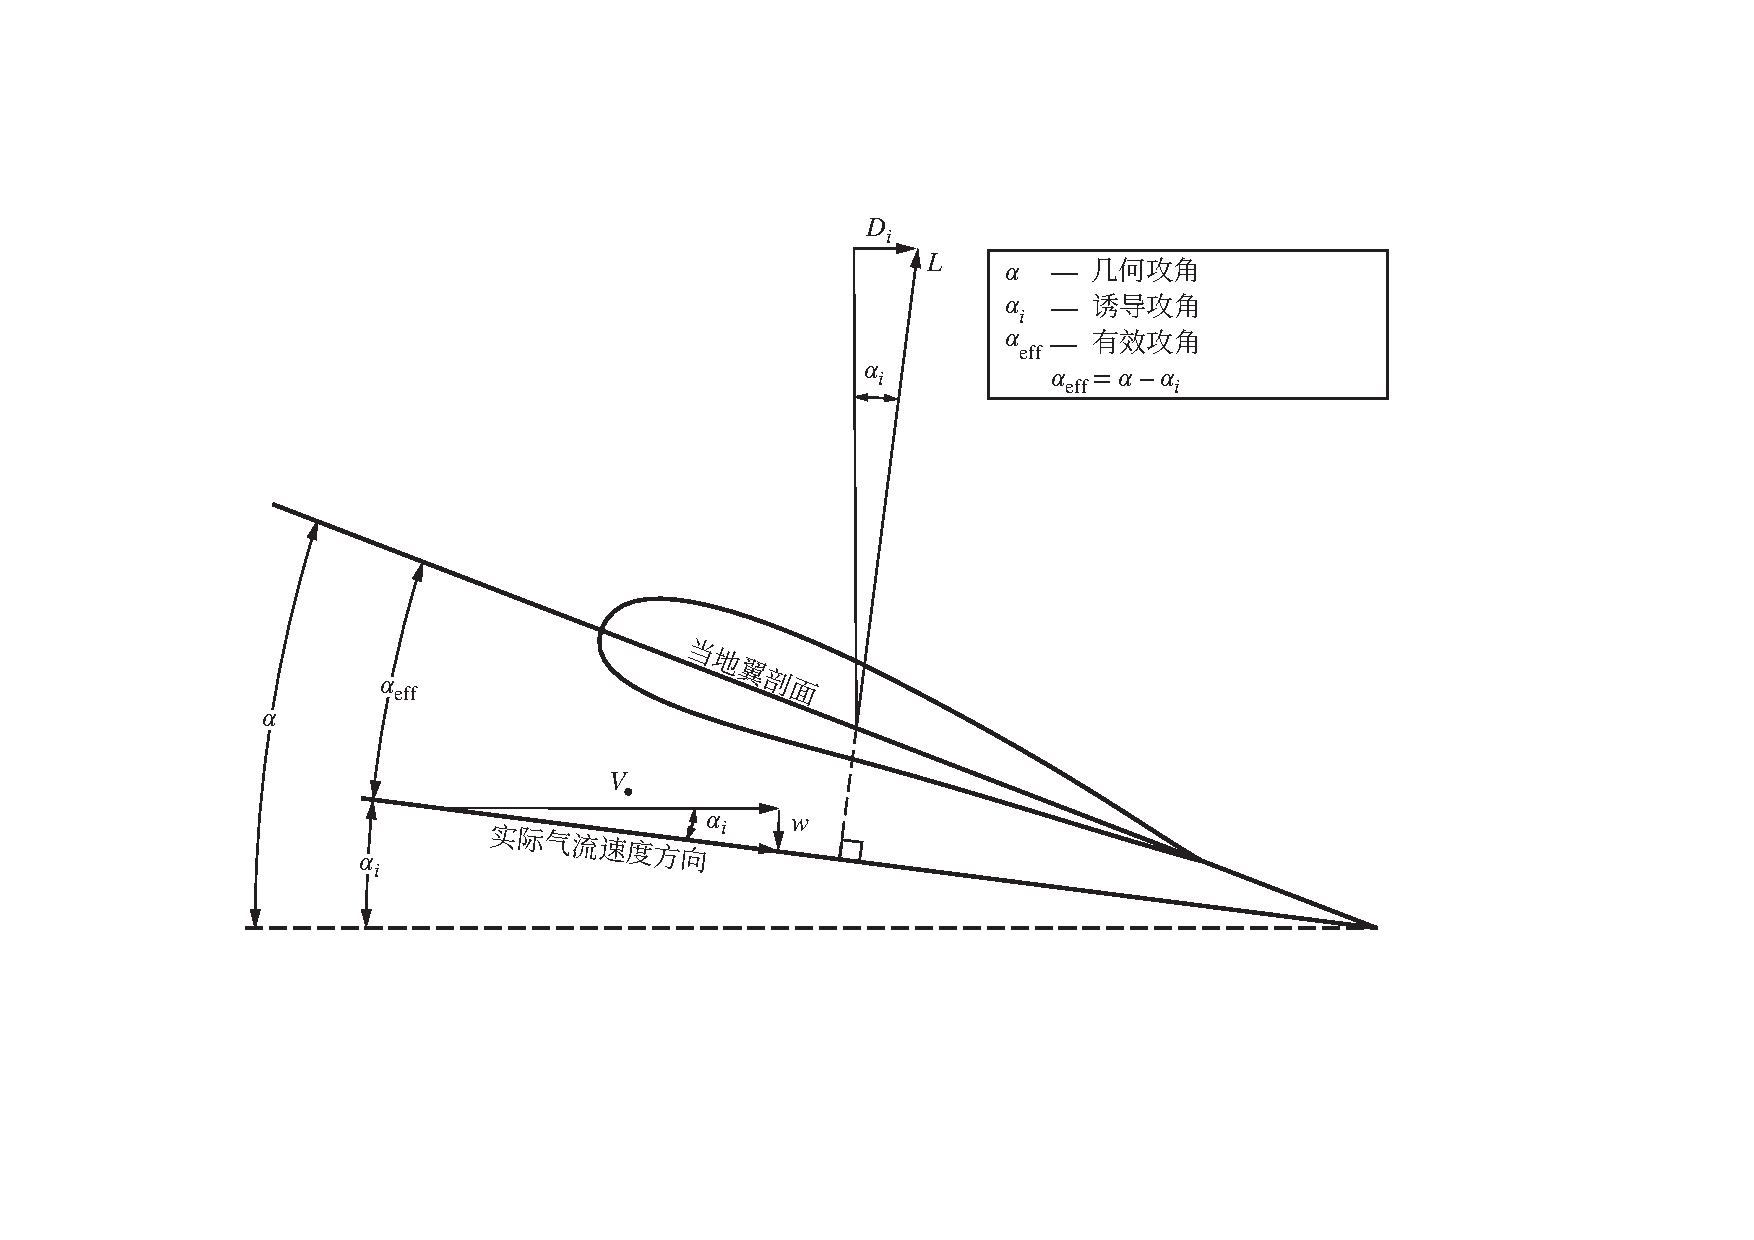
\includegraphics[height=10cm]{./aerodynamics/effective_attack.pdf}
  \caption{下洗对有限翼展机翼当地翼型截面的影响}
  \label{fig:effective_attack}
\end{figure}
当地气流的方向相对于自由来流的方向向下倾斜了$\alpha_i$角度,这个角度
叫做{\bfseries 诱导攻角(induced angle of attack)}。下洗流的存在,
使得当地气流方向向下倾斜,同时对当地翼有剖面主要有两个
影响,如下:
\begin{enumerate}
  \item 实际的迎角是当地气流的方向和当地翼型弦线的夹角,这个夹角
    叫做{\bfseries 有效迎角(effective angle of attack)},记作
    $\alpha_{eff}$。因此,即使机翼有着几何攻角$\alpha$,当地翼型的
    迎角实际上更下一些,即有效迎角。
    \[
      \alpha_{eff}=\alpha-\alpha_i
    \]
  \item 当地的升力向量垂直于当地气流方向,因此相较于原来的升力向量
    (竖直方向)落后了角度$\alpha_i$。结果是在自由来流的方向会有
    一个当地升力向量的分量。也就是说,这个阻力是因为下洗的原因产生
    的。这个阻力就被叫做{\bfseries 诱导阻力(induced drag)},记作
    $D_i$。
\end{enumerate}

升力向后倾斜是诱导阻力产生的一种解释,另外的两个解释如下:
\begin{enumerate}
  \item 翼尖涡诱导出来的速度,使得机翼上在自由来流的方向上压强不平衡
    产生了一个向后的力,这个力就是诱导阻力。在这种情况下,诱导阻力也是
    压差阻力的一种。
  \item 翼尖涡中包含了大量的平移和转动的内能,这部分能量必须来自于某个地方
    。事实上,这部分能量几乎都是由飞机的发动机提供的,而发动机是飞机唯一
    相关的动力来源。由于翼尖涡的能量没有任何用处,因此这种能量基本上
    已经丧失。实际上,发动机提供的进入涡流的额外动力就是发动机克服
    诱导阻力所需的额外动力。
\end{enumerate}

\begin{notice}
关于本章的符号问题

对于单位翼展上的升力,阻力,气动力矩,记作$L'$,$D'$,$M'$。
相应的升力系数,阻力系数,力矩系数,记作$c_l$,$c_d$,$c_m$。
对于三维机翼,比如有限翼展的机翼,升力,阻力,气动力矩
记作$L$,$D$,$M$。相应的升力系数,阻力系数,力矩系数
记作$C_L$,$C_D$,$C_M$。对于亚音速的机翼上阻力是诱导阻力$D_i$,
表面摩擦阻力$D_f$和压差阻力$D_P$的和。后面两个阻是因为粘性产生的,
它们的和叫做型阻。对于任何攻角,有限翼展的机翼的型阻系数都是
一样的。
\[
 c_d=\frac{D_f+D_P}{q_\infty S} 
\]
诱导阻力系数是
\[
  C_{D,i}=\frac{D_i}{q_\infty S}
\]
总的阻力系数是
\[
  C_D=c_d+C_{D,i}
\]
\end{notice}

\section{面涡,毕奥--萨伐尔定律和亥姆霍兹定理}
在前面,我们介绍了无限长的直线分布的面涡,实际上,面涡分布
也可以是曲线,沿着涡线积分,就可以得到涡量$\Gamma$,
也是涡强。

考虑涡线上一点的一段有向线段$\mathrm{d}\mathbf{l}$
,在任意一点$P$处,有向线段到该点的径矢是$\mathbf{r}$,
那么有向线段在$P$点处的诱导速度是
\[
  \mathrm{d}\mathbf{V}=\frac{\Gamma}{4 \pi}
  \frac{\mathrm{d}\mathbf{l}\times \mathbf{r}}{\lvert \mathbf{r}\rvert ^3}
\]
这就是毕奥--萨伐尔定律。这和磁场中的毕奥--萨伐尔定律
是一样的。一根无限长的直涡线在任意一点$P$处的诱导速度
是
\[
  V=\frac{\Gamma}{2 \pi h }
\]
其中,$h$是$P$点到涡线的距离。

亥姆霍兹定理的内容如下:
\begin{enumerate}
  \item 面涡的强度沿着它的长度方向是一个常数
  \item 面涡不能在流体中结束,必须在边界上结
    束或者形成一个闭合的路径
\end{enumerate}

下面介绍{\bfseries 升力分布(lift distribution)}的
概念。在给定位置$y_1$升力大小是$L'\left(y_1\right) $,
这个位置处的弦长和迎角分别是$c$和$\alpha$。现在
在另外一个位置$y_2$处的弦长和迎角可能会发生变化,
在这个位置的升力是$L'\left(y_2\right) $ 
\begin{notice}
大部分机翼的翼型的弦长都会随着位置发生变化,矩形
机翼除外;并且每个截面翼型的几何攻角也可能不同,
这是因为机翼有可能发生扭转了。如果翼根处的翼型的
几何攻击大于翼尖的几何攻击,叫做washout ,反之叫
做washin。这种情况叫做{\bfseries 几何扭转(geometrical twist)}。
另外,现代的机翼,不同截面的翼型也不同,所以
每个截面的零升迎角也不同,这叫做{\bfseries 气动扭转(aerodynamic twist)}。
\end{notice}
在不同位置处,单位翼展上的升力是不同的,这就是
机翼上沿着翼展方向上的单位翼展上的升力分布,即$L'=L'(y)$。
根据茹科夫斯基定理,我们知道
\[
  L'=L'(y)=\rho_\infty V_\infty \Gamma(y)
\]
在翼尖处,由于上下表面的压强平衡,所以在翼尖位置,即$y=-\frac{b}{2 }$和
$y= \frac{b}{2}$处的升力等于0 。

总的来说,本章的问题就是计算诱导阻力,总升力,
有限翼展机翼的升力分布。

\section{普朗特经典升力线理论}
普朗特认为,一个强度为$\Gamma$的面涡将被以
某种方式固定在流场中的某个固定位置,这个叫
做
{\bfseries 附着涡(bound vortex)}
,并且产生一个升力
$L'=\rho_\infty V_\infty \Gamma$
。与附着涡相反的是
{\bfseries 自由涡(free vortex)}
,它会随着同一个流体微团运动而遍及全流场。
用一个从
$y=-\frac{b}{2 }$
到
$y=\frac{b}{2 }$
的附着涡替换掉机翼。根据亥姆霍兹定理,涡线
不能再流场中结束,因此假设在翼尖的下游有两
条向无限远方向延伸的自由涡。因为附着涡和自
由涡叠加而形成的涡系形状上像一个马蹄,因此
叫做
{\bfseries 马蹄涡(horseshoe vortex)}。
附着涡不会在翼展这段位置上诱导出下洗的速度
,因此,下洗速度$w $都是由自由涡诱导出来的
。我们可以用毕奥萨伐尔定律计算出翼展上的诱
导速度
\[
  w(y)=-\frac{\Gamma}{4\pi(\frac{b}{2}+y)}
       -\frac{\Gamma}{4\pi(\frac{b}{2}-y)}
       =-\frac{\Gamma}{4\pi}\frac{b}{\left
     (\frac{b}{2}\right)^2-y^2}
\]

单个马蹄涡产生的下洗速度分布和实际情况并不
一致,并且在翼尖处诱导速度将接近无穷大,这
显然不合理。假设在翼展上分布由大量的马蹄涡
形成一个马蹄涡系,每个马蹄涡的附着涡长度都
不一样,并且强度也不一样,但是每条附着涡都
还是沿着一条直线分布的,这条线叫做
{\bfseries 升力线(lifting line)}。
这一部分请参考教材。
请记住尾涡的强度等于升力线上面涡强度的变化
。

如果叠加无穷多的马蹄涡,形成一个马蹄涡系,
这样沿翼展方向,面涡强度
$\Gamma$
就变成了一个连续分布的函数,也就是
$\Gamma=\Gamma(y)$
在微元长度上的面涡强度就是
\[
  \mathrm{d}\Gamma=\left(\frac{\mathrm{d}
  \Gamma}{\mathrm{d}y}\right)
  \mathrm{d}y
\]
相应地,尾涡的强度就等于
$\mathrm{d}\Gamma$
的变化。那么任意一点$y $处的涡强
$\mathrm{d}\Gamma$
在$y_0$ 处的诱导速度就是
\[
  \mathrm{d}w=-\frac{(\mathrm{d}\Gamma 
  / \mathrm{d}y)\mathrm{d}y}{4\pi(y_0-y)}
\]
这个速度是在$y $处的半无限长的自由涡在点
$y_0 $诱导出的下洗速度。这个负号表示速度方
向是向下的。在$y_0 $点的总诱导速度由下式给
出
\[
  w=-\frac{1}{4\pi}
  \int_{-\frac{b}{2}}^{\frac{b}{2 }}
  \frac{\left(\frac{\mathrm{d}\Gamma}{\mathrm{d}y}\right)}
  {y_0-y}\mathrm{d}y
\]
上式很重要,它给出了在$y_0 $处由所有自由涡
诱导出来的下洗速度。

从图\ref{fig:effective_attack}中,我们得到
诱导迎角的大小
\[
  \alpha_i(y_0)=\tan ^{-1}
  \left(\frac{-w(y_0) }{V_\infty}\right)
\]
一般来说,$w $远小于$V_\infty$,所以诱导迎
角也可以写成
\[
  \alpha_i(y_0)= -\frac{w(y_0) }{V_\infty}
\]
再将前面计算下洗速度的积分公式代入就可以得
到
\begin{empheq}[box=\widefbox]{equation*}
  \alpha_i(y_0)=\frac{1}{4\pi V_\infty}
  \int_{-\frac{b}{2 }}^{\frac{b}{2 }}
  \frac{\left(\frac{\mathrm{d}\Gamma}{\mathrm{d}y}\right) }
  {y_0-y}\mathrm{d}y
\end{empheq}
这样我们就可以通过涡强分布来计算诱导迎角的
大小。

根据前面所述的几何迎角和有效迎角之间的关系
,我们可以计算处有效迎角
\[
  \alpha_{eff}= \alpha-\alpha_i
  =\alpha-\frac{1}{4\pi V_\infty}
  \int_{-\frac{b}{2 }}^{\frac{b}{2 }}
  \frac{\left(\frac{\mathrm{d}\Gamma}{\mathrm{d}y}\right) }
  {y_0-y}\mathrm{d}y
\]
然后根据前面我们讨论的翼型的升力曲线,我们
就可以得到在$y_0 $处的升力系数
\[
  c_l=a_0\left(\alpha_{eff}(y_0)-\alpha_{L=0}\right)
  =2\pi\left(\alpha_{eff}(y_0)-\alpha_{L=0}\right)
\]
在任何情况下,零升迎角都是已知的,它只与翼
型有关。同样,升力不仅可以通过升力系数进行
计算,还可以用茹科夫斯基升力公式进行计算,
也就是
\[
  L'=\frac{1}{2}\rho_\infty V_\infty ^2 
  c(y_0)c_l
  = \rho_\infty V_\infty \Gamma\left(y_0\right) 
\]
于是我们又可以得到计算机翼单位翼展上升力系
数的第二个公式,即
\[
  c_l=\frac{2 \Gamma\left(y_0\right) }{V_\infty c(y_0) }
\]
所以有效攻角也可以用下式计算
\[
  \alpha_{eff}=\frac{\Gamma\left(y_0\right) }
  {\pi V_\infty c\left(y_0\right) }+\alpha_{L=0}
\]
带入到
\[
  \alpha=\alpha_{eff}+\alpha_i
\]
中,我们就得到了几何攻角的计算公式,即
\begin{empheq}[box=\widefbox]{equation*}
  \alpha(y_0)= 
  \frac{\Gamma(y_0) }{\pi V_\infty c(y_0) }+
  \alpha_{L=0}(y_0)+
  \frac{1}{4\pi V_\infty}
  \int _{-\frac{b}{2}}^{\frac{b}{2 }}
  \frac{\frac{\mathrm{d}\Gamma }{\mathrm{d}y}}
  {y_0-y}\mathrm{d}y
\end{empheq}
这就是普朗特升力线理论的基本方程。这表明了几何
迎角等于有效迎角加上诱导迎角。这个方程是一个积
分---微分方程,唯一的未知量就是$\Gamma $,其他
量都是已知的。

从基本方程得出$\Gamma=\Gamma(y_0)$的解给了我们
三个关于有限翼展机翼的基本性质,即:
\begin{enumerate}
  \item 升力分布可以从库塔--- 茹科夫斯基定理中
    得到,即
    \[
      L'(y_0)=\rho_\infty V_\infty \Gamma(y_0) 
    \]
  \item 总升力可以对第一点性质中的公式积分得到
    ,即
    \[
      L=\int_{-\frac{b}{2 }}^{\frac{b}{2}}L'(y)\mathrm{d}y
    \]
    或
    \[
      L=\rho_\infty V_\infty 
      \int_{-\frac{b}{2 }}^{\frac{b}{2}}\Gamma(y)\mathrm{d}y
    \]
    升力系数可以由下式给出
    \[
      C_L=\frac{L}{q_\infty S}=\frac{2}{V_\infty S}= 
      \int _{-\frac{b}{2}}^{\frac{b}{2}}\Gamma(y)\mathrm{d}y
    \]
  \item 从图\ref{fig:span}中,我们可以得到诱导
    阻力的计算公式,即
    \[
      D' _i=L' _i\sin \alpha_i
    \]
    因为诱导迎角很小,所以
    \[
      D' _i=L' _i\alpha_i
    \] 
    于是总的诱导阻力由下面的积分公式给出
    \[
      D_i=\int _{-\frac{b}{2}}
      ^{\frac{b}{2}}L'(y)\alpha_i(y)
      \mathrm{d}y 
    \]
    或
    \[
      D_i= \rho_\infty V_\infty 
      \int _{-\frac{b}{2}}
      ^{\frac{b}{2}}
      \Gamma(y)\alpha_i(y)\mathrm{d}y
    \]

    相应地,诱导阻力系数就是
    \[
      C_{D,i}=\frac{D_i}{q_\infty S}
      =\frac{2}{V_\infty S}
      \int _{-\frac{b}{2}}
      ^{\frac{b}{2}}
      \Gamma(y)\alpha_i(y)\mathrm{d}y
    \]
\end{enumerate}

\subsection{椭圆型升力分布}
考虑一个涡强分布,即
\[
  \Gamma(y)=\Gamma_0
  \sqrt{1-\left(\frac{2y}{b}\right)^2} 
\]
请记住:
\begin{enumerate}
  \item $\Gamma_0$是涡强的初始值,是在
    翼展中间的值
  \item 环量随着坐标$y $椭圆型地变化,
    单位翼展上的升力由下式给出
    \[
      L'(y)=\rho_\infty V_\infty 
      \Gamma_0
      \sqrt{1-\left(\frac{2y}{b }\right)^2} 
    \] 
    \item $\Gamma\left(-\frac{b}{2}\right)= 
      \Gamma\left(\frac{b}{2}\right) $,环量
      和升力在翼尖出等于0 。
\end{enumerate}

首先,我们先计算下洗,
\[
  \frac{\mathrm{d}\Gamma}{\mathrm{d}y}
  =-\frac{4\Gamma_0}{b^2}
  \frac{y}{\left(1-\frac{4y^2}{b^2}\right)^{\frac{1}{2}}}
\]
带入到下式中
\[
  w(y_0)=-\frac{1}{4\pi}
  \int _{-\frac{b}{2}}^{\frac{b}{2}}
  \frac{\mathrm{d}\Gamma / \mathrm{d}y}{y_0-y}\mathrm{d}y
\]
得到
\[
  w(y_0)=\frac{\Gamma_0}{\pi b^2}
  \int _{-\frac{b}{2}}^{\frac{b}{2}}
  \frac{y}{\left(1-\frac{4y^2}{b^2}\right)^{\frac{1}{2}}(y_0-y)}\mathrm{d}y
\]
作变量替换
\[
  y=\frac{b}{2}\cos \theta \qquad \mathrm{d}y=-\frac{b}{2}\sin \theta \mathrm{d}\theta
\]
上述积分就变成了
\[
  w(\theta_0)=-\frac{\Gamma_0}{2 \pi b }
  \int _0 ^\pi \frac{\cos \theta}{\cos \theta-\cos \theta_0}\mathrm{d} \theta
\]
计算得到
\[
  w(\theta_0)=-\frac{\Gamma_0}{2b}
\]
这结果表明,{\color{noteorange}\bfseries 对于椭圆型升力分布的机翼来说,
下洗速度是一个常数}。这个结论很有趣也很重要。
我们可以计算得到诱导迎角
\[
  \alpha_i=-\frac{w }{V_\infty }= \frac{\Gamma_0}{2 b V_\infty}
\]

\part{附录}
\appendix
%附录
%积分
% ! TEX root=../mechanics.tex

\chapter{积分}
\section{第一个积分}
\label{马赫波积分}
求积分
\[
	\int \frac{\sqrt{M^2-1}}{\left(1+\frac{\gamma-1}{2}M^2\right)M}\mathrm{d}M
\]
首先,换元,令$M=\sec \alpha$,得到$\mathrm{d}M=\tan \alpha \sec \alpha \mathrm{d}\alpha$,
则有$\tan \alpha=\sqrt{M^2-1}$,$\alpha=\arctan \sqrt{M^2-1}$
\begin{equation*}
	\begin{split}
		\begin{WithArrows}[code-before=\color{titleblue}]
			\int \frac{\sqrt{M^2-1}}{\left(1+\frac{\gamma-1}{2}M^2\right)M}\mathrm{d}M
			%\Arrow{$M=\sec \alpha$\\
			%   $\mathrm{d}M= \tan \alpha \sec \alpha \mathrm{d}\alpha$ }\\
			&=\int \frac{\tan^2 \alpha \cdot \sec \alpha }{\sec \alpha \left(1+\frac{\gamma-1}{2}\sec^2 \alpha\right)}\mathrm{d}\alpha\\
			&= \int \frac{\tan^2 \alpha }{1+\frac{\gamma-1}{2}\sec^2\alpha} \mathrm{d}\alpha
			\Arrow{分子分母同乘\\ $\cos^2\alpha$,并约化}\\
			&=\int \left(-1+\frac{\gamma+1 }{2\cos^2\alpha+\gamma-1}\right)\mathrm{d}\alpha
			\Arrow{
				$u=\tan \alpha$\\
				$\mathrm{d}\alpha=\frac{\mathrm{d}u}{1+u^2}$
			}\\
			&=-\alpha+\int \frac{\gamma+1 }{\frac{2}{1+u^2}+\gamma-1}\cdot \frac{\mathrm{d}u}{1+u^2}\\
			&=-\alpha +\int \frac{1}{\frac{\gamma-1}{\gamma+1 }u^2+1 }\mathrm{d}u\\
			&=-\alpha+\sqrt{\frac{\gamma+1 }{\gamma-1}} \int
			\frac{1}{\left(\sqrt{\frac{\gamma-1}{\gamma+1 }} u\right)^2+1}
			\mathrm{d}\left(\sqrt{\frac{\gamma-1 }{\gamma+1}}u\right)\\
			&=-\alpha+\sqrt{\frac{\gamma+1 }{\gamma-1 }} \arctan \sqrt{\frac{\gamma-1}{\gamma+1}}u\\
			&=\sqrt{\frac{\gamma+1 }{\gamma-1}} \arctan \sqrt{\frac{\gamma-1 }{\gamma+1 }\left(M^2-1\right)}-\arctan \sqrt{M^2-1}
		\end{WithArrows}
	\end{split}
\end{equation*}

\section{第二个积分}
\label{三角函数定积分}
{\color{titleblue}
证明定积分
\[
	\int _0^\pi \frac{\cos n \theta}{\cos \theta -\cos \theta_0}\,\mathrm{d}\theta=\frac{\pi \sin n\theta_0}{\sin \theta_0},\qquad n=0,1,2,\ldots
\]
}

积化和差公式
\[
	\begin{split}
		\cos \theta -\cos \theta_0 & =\cos\left(\frac{\theta+\theta_0}{2}+\frac{\theta-\theta_0}{2}\right)
		-\cos\left(\frac{\theta+\theta_0}{2}-\frac{\theta-\theta_0}{2}\right)                                   \\
		                           & =-2\sin \frac{\theta+\theta_0}{2}\sin \frac{\theta-\theta_0}{2}
	\end{split}
\]
\[
	\begin{split}
		\sin \theta & =\sin\left(\frac{\theta+\theta_0}{2}+\frac{\theta-\theta_0}{2}\right)     \\
		            & =\cos \frac{\theta+\theta_0}{2}\sin \frac{\theta-\theta_0}{2}+
		\cos \frac{\theta-\theta_0}{2}\sin \frac{\theta+\theta_0}{2}
	\end{split}
\]
那么
\[
	\frac{2\sin \theta_0}{\cos \theta-\cos \theta_0}=\cot \frac{\theta_0-\theta}{2}+\cot \frac{\theta_0+\theta}{2}
\]
考虑积分
\[
	I=\int _0^\pi \frac{\cos n \theta}{\cos \theta -\cos \theta_0}\sin \theta_0 \,\mathrm{d}\theta
	=\int _0^\pi \left(\cot \frac{\theta_0-\theta}{2}+\cot \frac{\theta_0+\theta}{2}\right)\cos n \theta \,\mathrm{d} \theta
\]
而
\[
	\int _0^\pi \cot \frac{\theta_0-\theta}{2} \cos n \theta \,\mathrm{d}\theta
	\xlongequal{用-\theta 换\theta}
	\int _{-\pi}^0 \cot \frac{\theta_0+\theta}{2} \cos n \theta\,\mathrm{d}\theta
\]
\[
	\int _0^\pi \cot \frac{\theta_0+\theta}{2} \cos n \theta \,\mathrm{d}\theta
	\xlongequal{用-\theta 换\theta}
	\int _{-\pi}^0 \cot \frac{\theta_0-\theta}{2} \cos n \theta \,\mathrm{d}\theta
\]
\[
	\int _0^\pi \left(\cot \frac{\theta_0-\theta}{2}+\cot \frac{\theta_0+\theta}{2}\right)\cos n \theta \,\mathrm{d} \theta=
	\int _{-\pi}^0 \left(\cot \frac{\theta_0+\theta}{2}+\cot \frac{\theta_0-\theta}{2}\right)\cos n \theta \,\mathrm{d} \theta
\]
那么
\[
	\begin{split}
		\int _0^\pi\left(\cot \frac{\theta_0-\theta}{2}+\cot \frac{\theta_0+\theta}{2}\right)\cos n \theta \,\mathrm{d}\theta
		 & =
		\int _0^\pi \cot \frac{\theta_0-\theta}{2}\cos n \theta \,\mathrm{d} \theta+
		\int _0^\pi \cot \frac{\theta_0+\theta}{2}\cos n \theta \,\mathrm{d} \theta \\
		 & =
		\int _{-\pi}^0 \cot \frac{\theta_0+\theta}{2}\cos n \theta \,\mathrm{d} \theta+
		\int _0^\pi \cot \frac{\theta_0+\theta}{2}\cos n \theta\,\mathrm{d} \theta \\
		 & =
		\int _{-\pi}^\pi \cot \frac{\theta_0+\theta}{2}\cos n \theta \,\mathrm{d} \theta
	\end{split}
\]
所以
\begin{equation*}
	\begin{split}
		\begin{WithArrows}
			I&=\frac{1}{2}\int _0^\pi \left(\cot \frac{\theta_0+\theta}{2}+\cot \frac{\theta_0-\theta}{2}\right)\cos n \theta \,\mathrm{d}\theta \\
			&=\frac{1}{2}\int _{-\pi}^\pi \cot \frac{\theta_0+\theta}{2} \cos n \theta \,\mathrm{d} \theta 
      \Arrow{$t=\theta+\theta_0$}\\ 
      &=\frac{1}{2}\int _{\theta_0-\pi}^{\theta+\pi} \cos n \left(t-\theta_0\right) \cot \frac{t}{2}\,\mathrm{d} t  
      \Arrow{
      	展开$\cos n (t-\theta_0)$}\\ 
      &=\frac{1}{2}\int _{\theta-\pi}^{\theta_0+\pi} \left(\cos nt \cos n \theta_0 +\sin nt \sin n \theta_0 \right)\cot \frac{t}{2}\,\mathrm{d} t  \\ 
      &=\frac{\cos n \theta_0}{2} \int _{\theta_0-\pi}^{\theta_0+\pi} \cos nt \cot \frac{t}{2}\,\mathrm{d}t+
      \frac{\sin n \theta_0}{2} \int _{\theta_0-\pi}^{\theta_0+\pi} \sin nt \cot \frac{t}{2} \,\mathrm{d} t  
			\end{WithArrows}
	\end{split}
\end{equation*}
其中$\sin n \theta_0$和$\cos n \theta_0$都是和积分变量无关的
常数。

下证积分
\[
  \int _{\theta_0-\pi}^{\theta_0+\pi} \cos nt \cot \frac{t}{2} \,\mathrm{d}t=0,\qquad n=1,2, \ldots 
\]
显然
\[
  \int _{\theta_0-\pi}^{\theta_0+\pi} \sin nt\,\mathrm{d}t=0,\qquad n=1,2, \ldots 
\]
而积分
\[
  \begin{split}
  \int _{\theta_0-\pi}^{\theta_0+\pi} \sin (n-1)t \cos t \,\mathrm{d}t 
  &=\int _{\theta_0-\pi}^{\theta_0+\pi} \sin (n-1)t \,\mathrm{d} \sin t\\  
  &=\sin (n-1)t \sin t\bigg| _{\theta_0-\pi}^{\theta_0+\pi}-
    \int _{\theta_0-\pi}^{\theta_0+\pi} \sin t (n-1) \cos (n-1)t \,\mathrm{d}t \\ 
  &=(n-1)\int _{\theta_0-\pi}^{\theta_0+\pi} \cos (n-1)t \,\mathrm{d} \cos t \\
  &=(n-1) \cos t \cos (n-1)t \bigg| _{\theta_0-\pi}^{\theta_0+\pi}+
    \int _{\theta_0-\pi}^{\theta_0+\pi} (n-1)^2 \sin (n-1)t \cos t \,\mathrm{d} t \\
  &=(n-1)^2\int _{\theta_0-\pi}^{\theta_0+\pi} \sin (n-1)t \cos t \,\mathrm{d}t
  \end{split}
\]
所以积分
\[
  \int _{\theta_0-\pi}^{\theta_0+\pi} \sin (n-1)t \cos t \,\mathrm{d}t =0
\]
同理可证下面积分
\[
  \int _{\theta_0-\pi}^{\theta_0+\pi} \sin (n-1)t \sin t \,\mathrm{d}t=0
\]
\[
  \int _{\theta_0-\pi}^{\theta_0+\pi} \cos (n-1)t \cos t \,\mathrm{d}t=0
\]
\[
  \int _{\theta_0-\pi}^{\theta_0+\pi} \cos (n-1)t \sin t \,\mathrm{d}t=0
\]
于是
\[
  \begin{split}
    \cos nt \cdot \cot \frac{t}{2}
    &=\cos nt \frac{\cos \frac{t}{2}}{\sin \frac{t}{2}}\\ 
    &=\cos nt \frac{\cos ^2 \frac{t}{2}}{\sin \frac{t}{2}\cos \frac{t}{2}}\\ 
    &=\cos nt \frac{1+\cos t }{\sin t}\\
    &=\cos [(n-1)t+t] \frac{1+\cos t }{\sin t }\\
    &=\left[\cos (n-1)t \cos t -\sin (n-1)t \sin t\right]\frac{1+\cos t }{\sin t}\\ 
    &=\frac{\cos (n-1)t \cos t (1+\cos t)}{\sin t}-\sin (n-1)t -\sin(n-1)t \cos  t
  \end{split}
\]
记$I_n=\int_{\theta_0-\pi}^{\theta_0+\pi} \cos nt \cot \frac{t}{2}\, \mathrm{d}t$,那么
\[
  \begin{split}  
    I_1&=\int _{\theta_0-\pi}^{\theta_0+\pi} \cos t \cot \frac{t}{2}\,\mathrm{d}t \\
       &=\int _{\theta_0-\pi}^{\theta0+\pi} \cos t \frac{1+\cos t}{\sin t}\,\mathrm{d}t \\ 
       &=\int _{\theta_0-\pi}^{\theta_0+\pi} \frac{\cos t +\cos ^2 t }{\sin t}\,\mathrm{d} t \\ 
       &=\int _{\theta_0-\pi}^{\theta_0+\pi} \frac{\cos t +1- \sin t ^2 t}{\sin t}\, \mathrm{d}t\\ 
       &=\int _{\theta_0-\pi}^{\theta_0+\pi} \left(\cot \frac{t}{2} +\sin t \right)\,\mathrm{d}t \\
       &=0
  \end{split}
\]
所以
\begin{align*}
    I_n=
    \int _{\theta_0-\pi}^{\theta_0+\pi} \cos nt \cot \frac{t}{2} \,\mathrm{d} t 
    &=\int _{\theta_0-\pi}^{\theta_0+\pi} \frac{\cos (n-1)t \cos t (1+\cos t)}{\sin t}\,\mathrm{d}t
    -
    \int _{\theta_0-\pi}^{\theta_0+\pi} \sin (n-1)t \,\mathrm{d}t \\ 
    & \quad
    -
    \int _{\theta_0-\pi}^{\theta_0+\pi} \sin (n-1)t \cos t \,\mathrm{d}t\\ 
    &=\int _{\theta_0-\pi}^{\theta_0+\pi} \frac{\cos (n-1)t \cos t (1+\cos t)}{\sin t} \,\mathrm{d} t\\ 
    &=\int _{\theta_0-\pi}^{\theta_0+\pi} \frac{\cos (n-1)t (\cos t +\cos ^2 t)}{\sin t} \,\mathrm{d}t\\ 
    &=\int _{\theta_0-\pi}^{\theta_0+\pi} \frac{\cos (n-1)t (\cos t +1- \sin ^2 t )}{\sin t}\,\mathrm{d}t \\ 
    &=\int _{\theta0-\pi}^{\theta_0+\pi} \frac{(1+\cos t)\cos (n-1)t }{\sin t}\,\mathrm{d}t
    -\int _{\theta_0-\pi}^{\theta_0+\pi} \cos (n-1)t \sin t \,\mathrm{d}t \\ 
    &=\int _{\theta_0-\pi}^{\theta_0+\pi} \frac{(1+\cos t)\cos (n-1)t }{\sin t}\,\mathrm{d}t \\ 
    &=I_{n-1}
\end{align*}
所以$I_n=I_{n-1}=\cdots =I_1=0$.
同上可证
\[
  \int _{\theta_0-\pi}^{\theta_0+\pi} \sin nt \cot \frac{t}{2} \,\mathrm{d}t =
  \int _{\theta_0-\pi}^{\theta_0+\pi} \sin (n-1)t \, \cot \frac{t}{2}\,\mathrm{d}t
\]
而
\[
  \int _{\theta_0-\pi}^{\theta_0+\pi} \sin t \, \cot \frac{t}{2} \,\mathrm{d} t =2\pi
\]
所以
\[
  \int _{\theta_0-\pi}^{\theta_0+\pi} \sin nt \, \cot \frac{t}{2}\,\mathrm{d} t =2\pi
\]
所以
\[
  I=\frac{\sin n \theta_0}{2} \int _{\theta_0-\pi}^{\theta_0+\pi} \sin nt \cot \frac{t}{2}\, \mathrm{d} t 
  =\pi \sin n \theta_0
\]
原积分
\[
  \int _0^{\pi} \frac{\cos n \theta}{\cos \theta -\cos \theta_0}\,\mathrm{d}t =
  \frac{\pi \sin n \theta_0}{\sin \theta_0}
\]

\section{第三个积分}
{
  \color{titleblue}
  证明
  \[
    \int _0^\pi \frac{\sin n \theta\,\sin \theta}{\cos \theta - \cos \theta_0}\,
    \mathrm{d} \theta=-\pi \cos n \theta_0,\qquad n=1,2, \ldots 
  \]
}
由积化和差公式
\[
  \sin n \theta \sin \theta =\frac{1}{2}\left[\cos (n-1)\theta -\cos (n+1)\theta\right]
\]
所以原积分
\[
  \begin{split}
    I=\int _0^\pi \frac{\sin n \theta \sin \theta}{\cos \theta -\cos \theta_0}\,\mathrm{d}\theta
    &=\frac{1}{2} \int _0^\pi \frac{\cos (n-1) \theta}{\cos \theta-\cos \theta_0}\,\mathrm{d}\theta
    -\frac{1}{2}\int _0^\pi \frac{\cos (n+1) \theta}{\cos \theta -\cos \theta_0}\, \mathrm{d} \theta\\ 
    &=\frac{1}{2} \left(\frac{\pi \sin (n-1)\theta_0}{\sin \theta_0}-\frac{\pi \sin (n+1)\theta_0}{\sin \theta_0}\right)\\ 
    &=-\pi \cos n \theta_0
  \end{split}
\]

% ! TEX root = ../mechanics.tex

\chapter{开尔文环量定理证明}
\label{kelvin theroem}
考虑无粘不可压流动,由环量定义有
\[
	\Gamma=\oint _c \mathbf{V}\cdot \mathrm{d} \mathbf{s}
\]
由于力学中,函数的性质都很好,所以微分运算和积分运算可以
直接交换次序。即
\[
	\begin{split}
		\frac{\mathrm{D} \Gamma}{\mathrm{D}t } & =\frac{\mathrm{D} }{\mathrm{D} t }\oint _c \mathbf{V} \cdot \mathrm{d}\mathbf{s}  \\
		                                       & =\oint _c \frac{\mathrm{D}}{\mathrm{D} t}(\mathbf{V}\cdot \mathrm{d} \mathbf{s})  \\
		                                       & =\oint _c \frac{\mathrm{D} \mathbf{V} }{\mathrm{D} t}\cdot \mathrm{d}\mathbf{s} +
		\mathbf{V}\cdot \frac{\mathrm{D}(\mathrm{d}\mathbf{s})}{\mathrm{D} t}
	\end{split}
\]
因为
\[
	\frac{\mathrm{D}(\mathrm{d}\mathbf{s})}{\mathrm{D}t}=\mathrm{d}\mathbf{V}
\]
V是一个单值函数,所以
\[
	\begin{split}
		\oint _c \mathbf{V} \cdot \frac{\mathrm{D}(\mathrm{d}\mathbf{s})}{\mathrm{D}t} & =
		\oint _c \mathbf{V}\cdot \mathrm{d}\mathbf{V}                                       \\
		                                                                               & =
		\oint _c (\mathrm{d} \frac{V^2}{2})                                                 \\
		                                                                               & =0
	\end{split}
\]
所以
\[
	\frac{\mathrm{D} \Gamma}{\mathrm{D}t}=\oint _c \frac{\mathrm{D} \mathbf{V}}{\mathrm{D}t}\cdot \mathrm{d}\mathbf{s}
\]
由动量方程,$\frac{\mathrm{D}\mathbf{V}}{\mathrm{D}t}$是加速度,也即单位质量流体受到的合外力。
所以
\[
  \frac{\mathrm{D}\mathbf{V}}{\mathrm{D}t}=-\frac{1}{\rho}\nabla P
\]
而
\[
  \begin{split}
  \nabla P \cdot \mathrm{d}\mathbf{s}&=(\frac{\partial P }{\partial x},\frac{\partial P}{\partial y},
  \frac{\partial P}{\partial z})\cdot (\mathrm{d}x,\mathrm{d}y,\mathrm{d}z)\\ 
                                     &=\frac{\partial P }{\partial x}\mathrm{d}x+
                                     \frac{\partial P}{\partial y}\mathrm{d}y+
  \frac{\partial P}{\partial z}\mathrm{d}z\\
                                     &=\mathrm{d}P(全微分定义)
  \end{split}
\]
于是
\[
  \begin{split}
    \frac{\mathrm{D} \mathbf{V}}{\mathrm{D} t}\cdot \mathrm{d}\mathbf{s}&=
    -\frac{1}{\rho}\nabla P \cdot \mathrm{d}\mathbf{s}\\                                                                      &=
     -\frac{1}{\rho}\mathrm{d}P
\end{split}
\]
于是
\[
  \oint _c 
    \frac{\mathrm{D} \mathbf{V}}{\mathrm{D} t}\cdot \mathrm{d}\mathbf{s}=
    \oint _c 
     -\frac{1}{\rho}\mathrm{d}P
     =0
\]
其中$\rho=常数$或者$\rho=\rho(P)$,即为不可压流动,或者是密度只是压强的函数的流动。


\end{document}
